\section*{Introduction}\index{Pterygota}\index{Pterygota}
In the insect phylogeny and fossil record we observe several adaptive radiations---\textit{i.e.}, events where the emergence of some key innovation or opportunity facilitated the rapid diversification of new forms. The emergence of wings is arguably the most important of these key innovations. The origin of these structures and the selective forces that acted on early versions of wings remain enigmatic. We will discuss hypotheses of the origin of wings before moving on to \textbf{Paleoptera} and the neopteran order \textbf{Plecoptera}.

\section*{Insecta: Pterygota}
We're now looking at insects that have \latinword{wings}, which are usually present as two pairs: fore wings, which articulate with the mesothorax, and hind wings, which articulate with the metathorax.\vspace{3mm}

\begin{theo}
{}Why is the thoracic integument so heavily sclerotized, relative to other body parts and those structures in non-pterygote hexapods? What are the consequences of this phenotype?
\end{theo}

\section*{Pterygota: Paleoptera}
In the next two orders, the wing base inhibits wing folding---\textit{i.e.}, the wings are held out or vertically over the thorax when at rest. The latest evidence indicates that these two orders comprise a monophyletic group, called Paleoptera.

\section{Ephemeroptera (mayflies)}\index{Ephemeroptera}%Ephemeridae in Penns Creek; add Caenidae or Leptohyphidae for operculate gills (protection in turbid water)

\subsection{Naiads}
Mayflies are aquatic in their immature stages, which are usually referred to as naiads or larvae (Not to be confused with the immature stages of holometabolous insects; more on that later.) Mayflies spend the vast majority of their lives as naiads, and we can see numerous adaptations for feeding and locomotion in this stage. Examine naiads of the following families, which should give you a sense of the phenotypic variation in Ephemeroptera: \textbf{Baetidae}, \textbf{Heptageniidae}, and \textbf{Ephemeridae}.\\\index{Baetidae}\index{Heptageniidae}\index{Ephemeridae}

\begin{figure}[ht!]
    \centering
    \begin{subfigure}[ht!]{0.6\textwidth}
        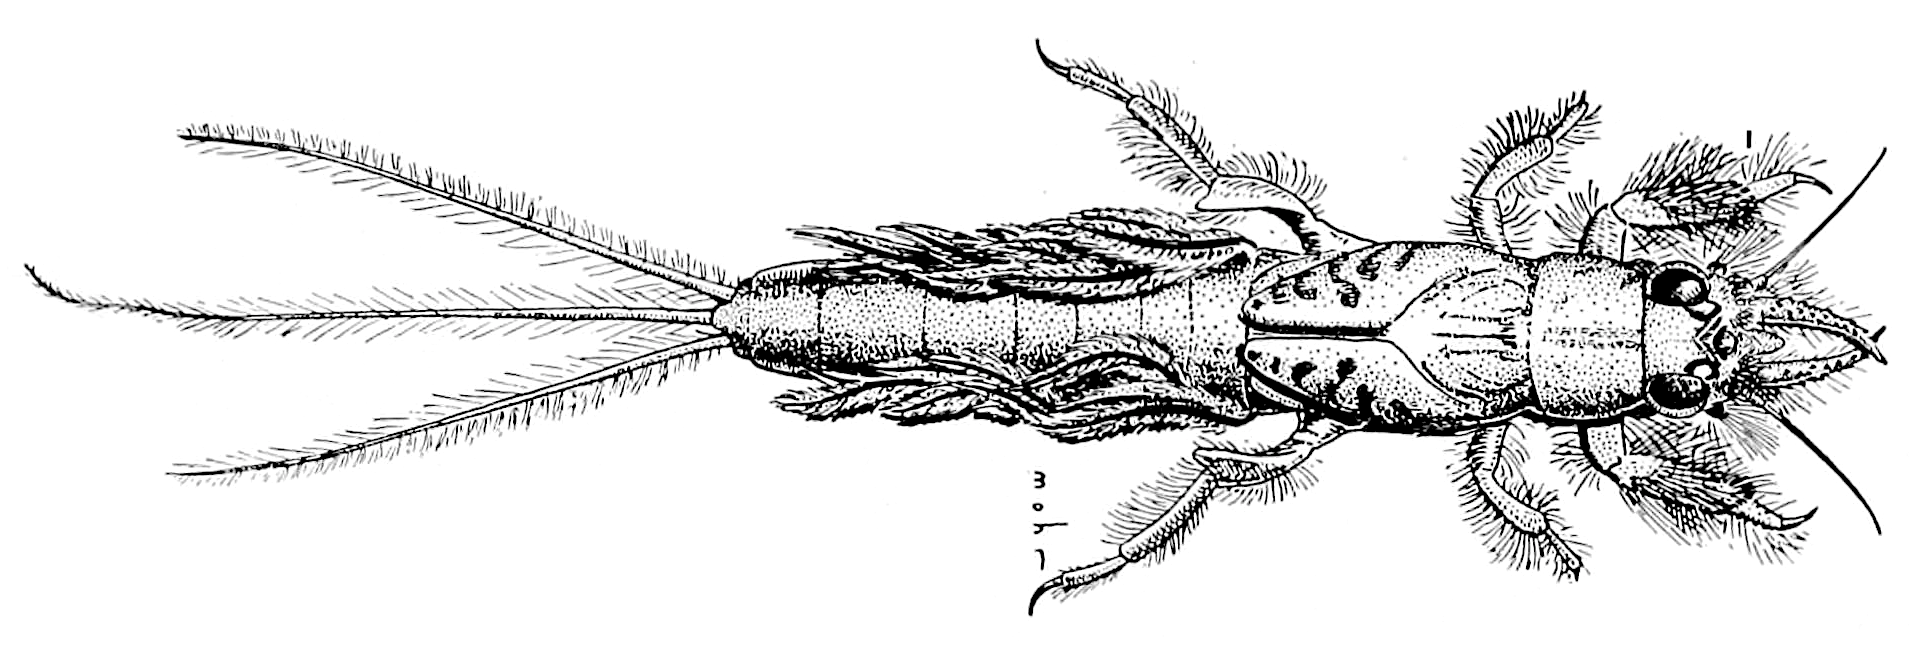
\includegraphics[width=\textwidth]{paleoptera/ephemNaiad}
        \caption{}
        \label{fig:ephemeridlarva}
    \end{subfigure}
    \hfill
    \begin{subfigure}[ht!]{0.25\textwidth}
        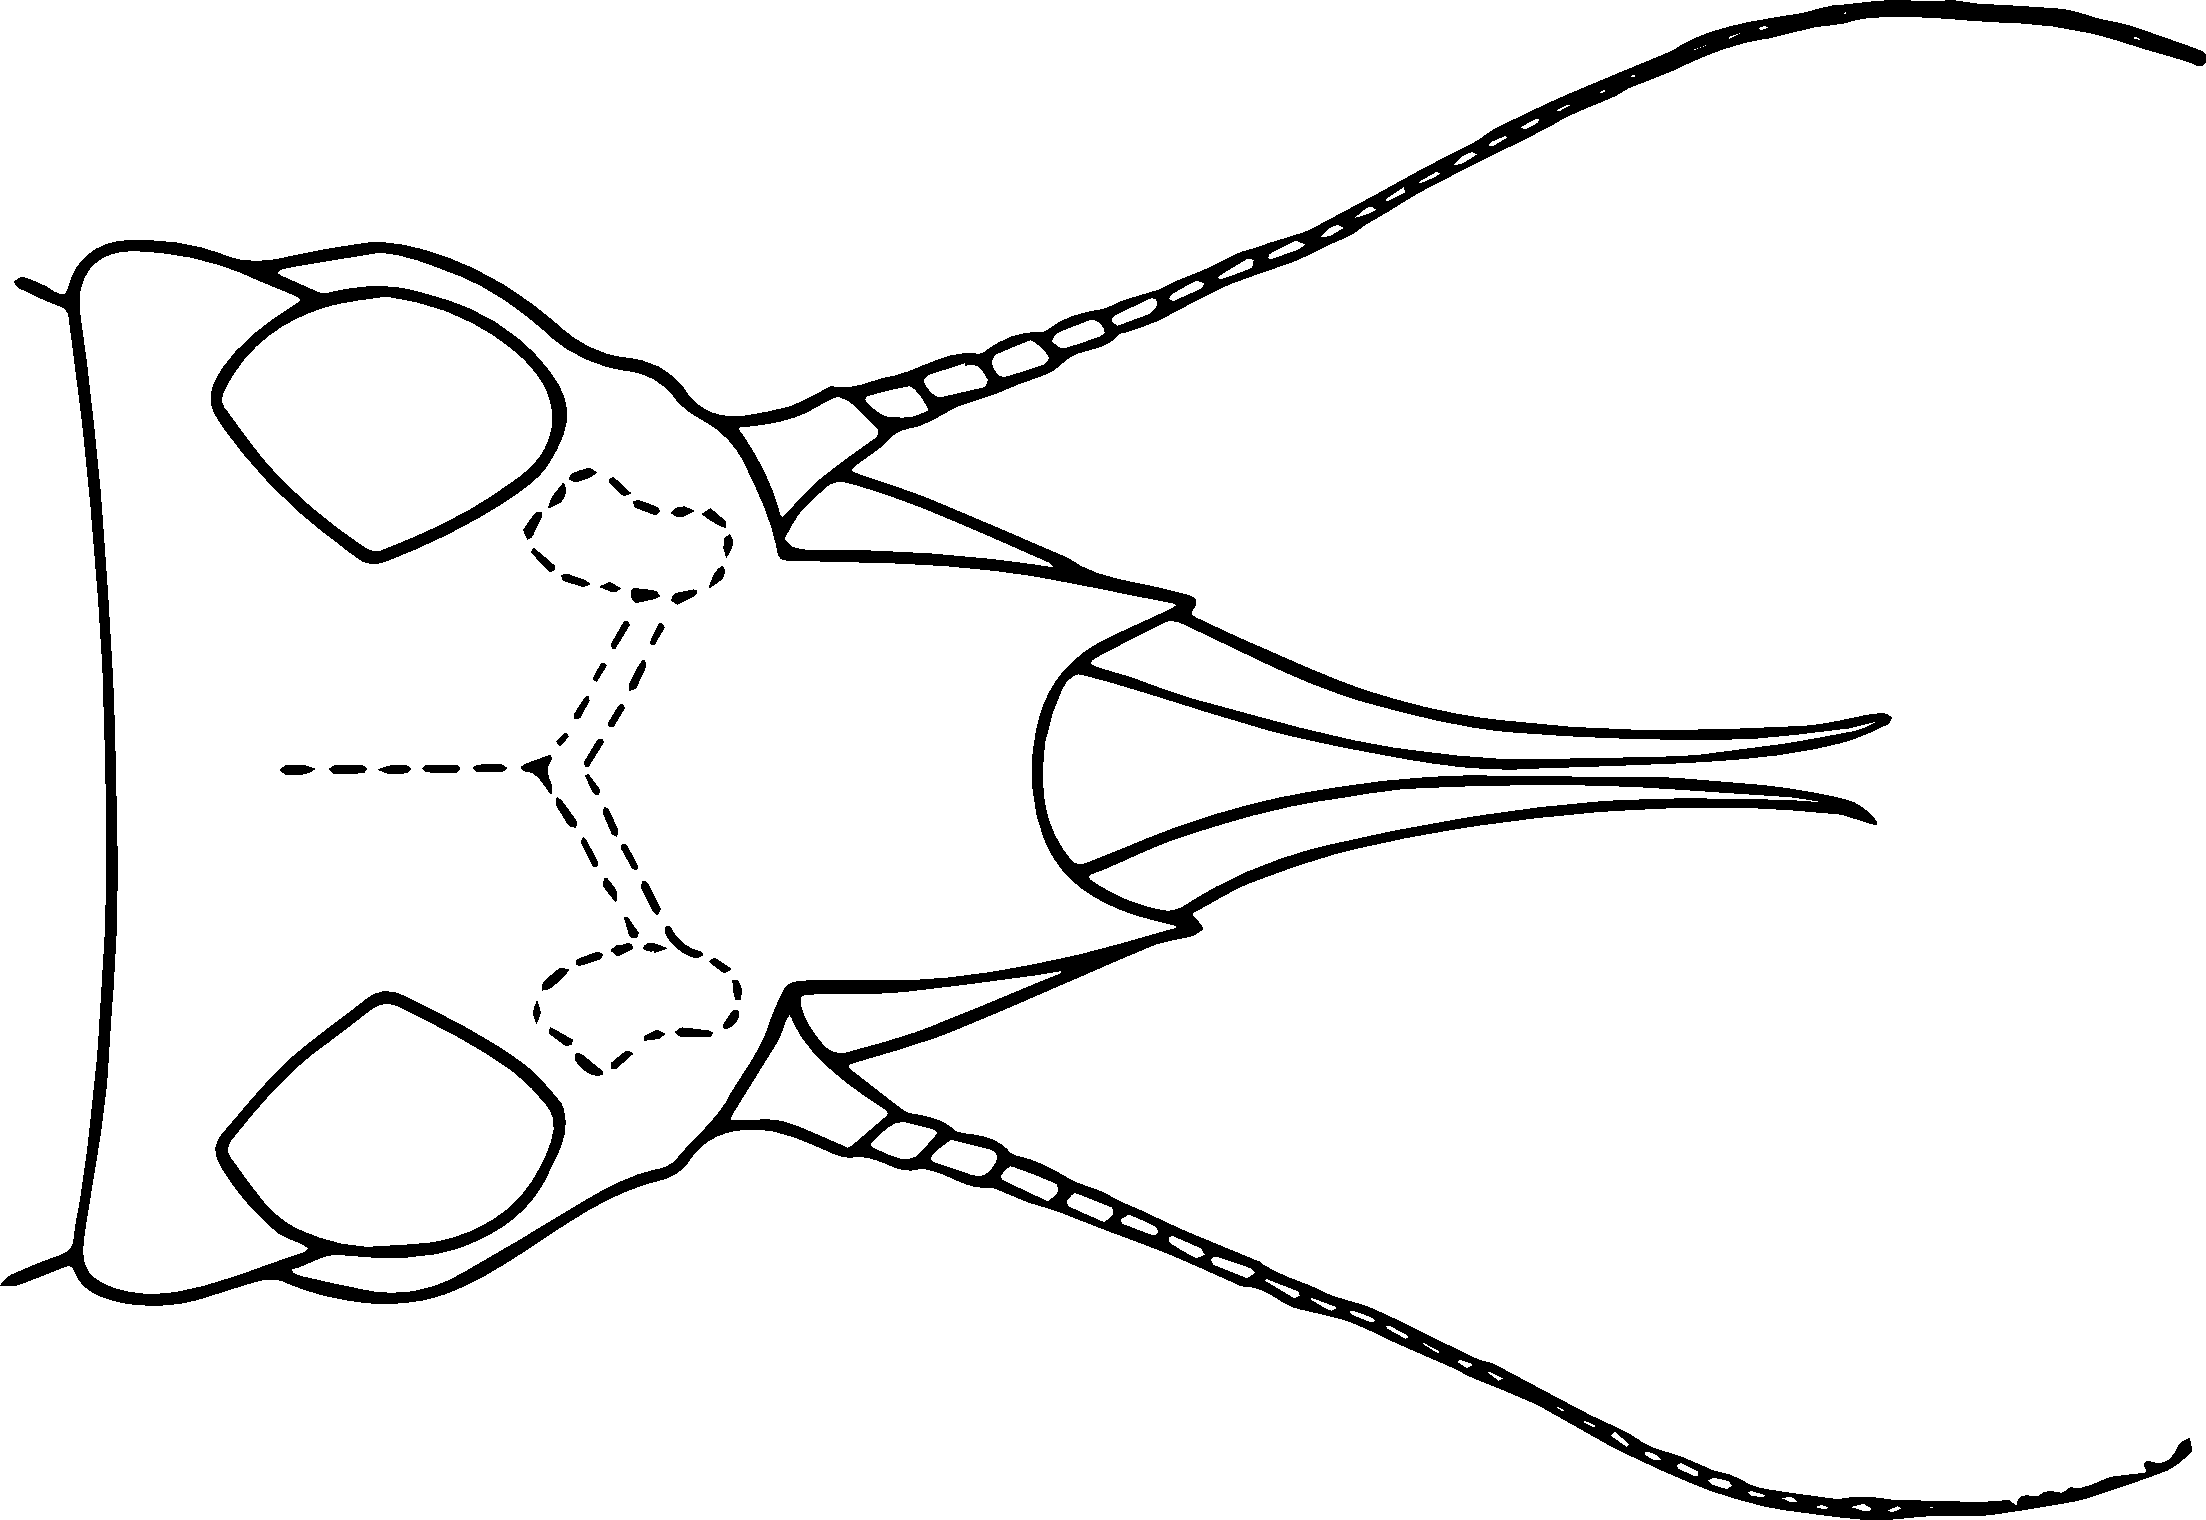
\includegraphics[width=\textwidth]{paleoptera/ephemNaiadHead}
        \caption{}
        \label{fig:ephemeridlarvahead}
    \end{subfigure}
    \caption{Ephemeridae naiad \textbf{(a)} habitus \citep[modified from][Fig. 59]{bhlpart97188ephem}; \textbf{(b)} head \citep[redrawn from][Fig. 50]{bhlpart97188ephem}}
    \label{fig:ephemeridLarvae}
\end{figure}

\begin{theo}
{}The bodies and head shapes of these mayflies yield clues about their life histories. Can you predict where each family is typically found and how eat it eats and moves through the water?\vspace{3mm}

\noindent{}Can you find evidence of developing wings? Describe your observations.
\end{theo}

\begin{figure}[ht!]
  \centering
    \reflectbox{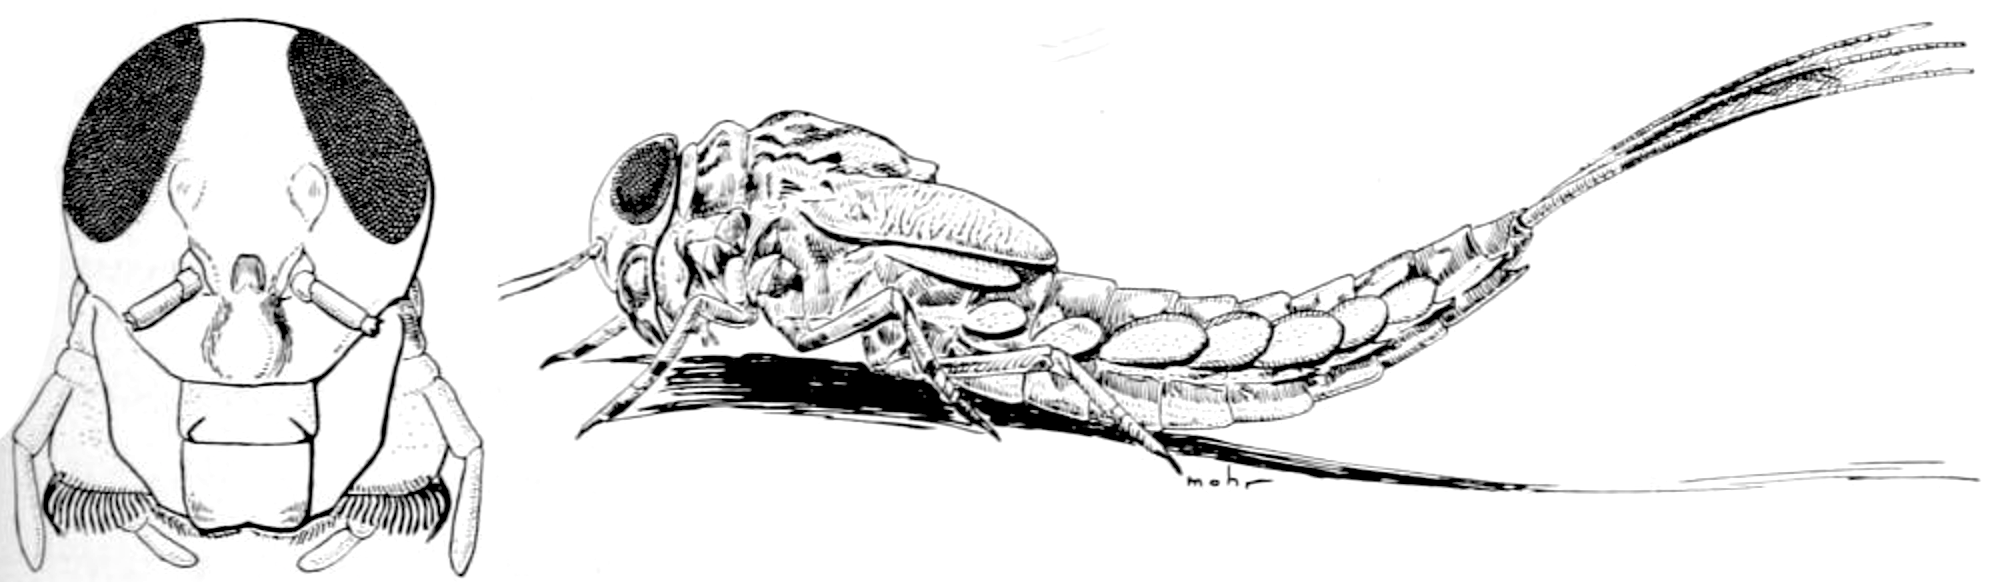
\includegraphics[width=0.7\textwidth]{paleoptera/baetidNaiad}}
  \caption{Baetidae naiad \citep[modified from][Fig. 240]{bhlpart97188ephem}}
  \label{fig:baetidNaiad}
\end{figure}

\begin{figure}[ht!]
  \centering
    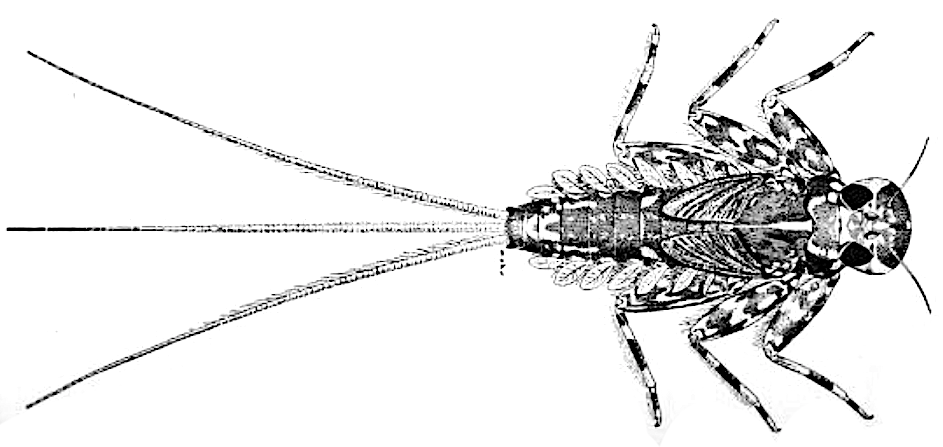
\includegraphics[width=0.6\textwidth]{paleoptera/heptageniidNaiad}
  \caption{Heptageniidae naiad \citep[modified from][Fig. 360]{bhlpart97188ephem}}
  \label{fig:heptageniidNaiad}
\end{figure}
\FloatBarrier

\subsection{Adults}
\noindent{}Wing venation and appendage traits offer important characters for family-level diagnosis of adults. See if you can understand the traits listed below characters, which could be used to recognize adults of three common families in the northeastern US: \textbf{Ephemeridae}, \textbf{Heptageniidae}, and \textbf{Baetidae}. Note that there are many other common mayfly families in this part of the world!%add diagnostic traits for adults at the order level!!!

\subsubsection{Ephemeridae (burrower mayflies, drakes)}\index{Ephemeridae}
\noindent{}\textit{Diagnostic characters:} Male compound eye round, unmodified; cubital intercalaries (between CuA and CuP) in fore wing not present as 2 parallel pairs; \texorpdfstring{MP\textsubscript{2}}{ }{ }of fore wing sharply angled towards Cu proximally; hind wing large, visible, with many veins; hind leg tarsus with 3-4 tarsomeres; apex of abdomen with 2--3 long appendages.\vspace{3mm}

\noindent{}\textit{Natural history:} Naiads have fossorial legs, which they use to burrow in substrate. They scavenge or predate on other arthropods. There are approximately 150 described spp. worldwide.\vspace{3mm}

\begin{figure}[ht!]
    \centering
       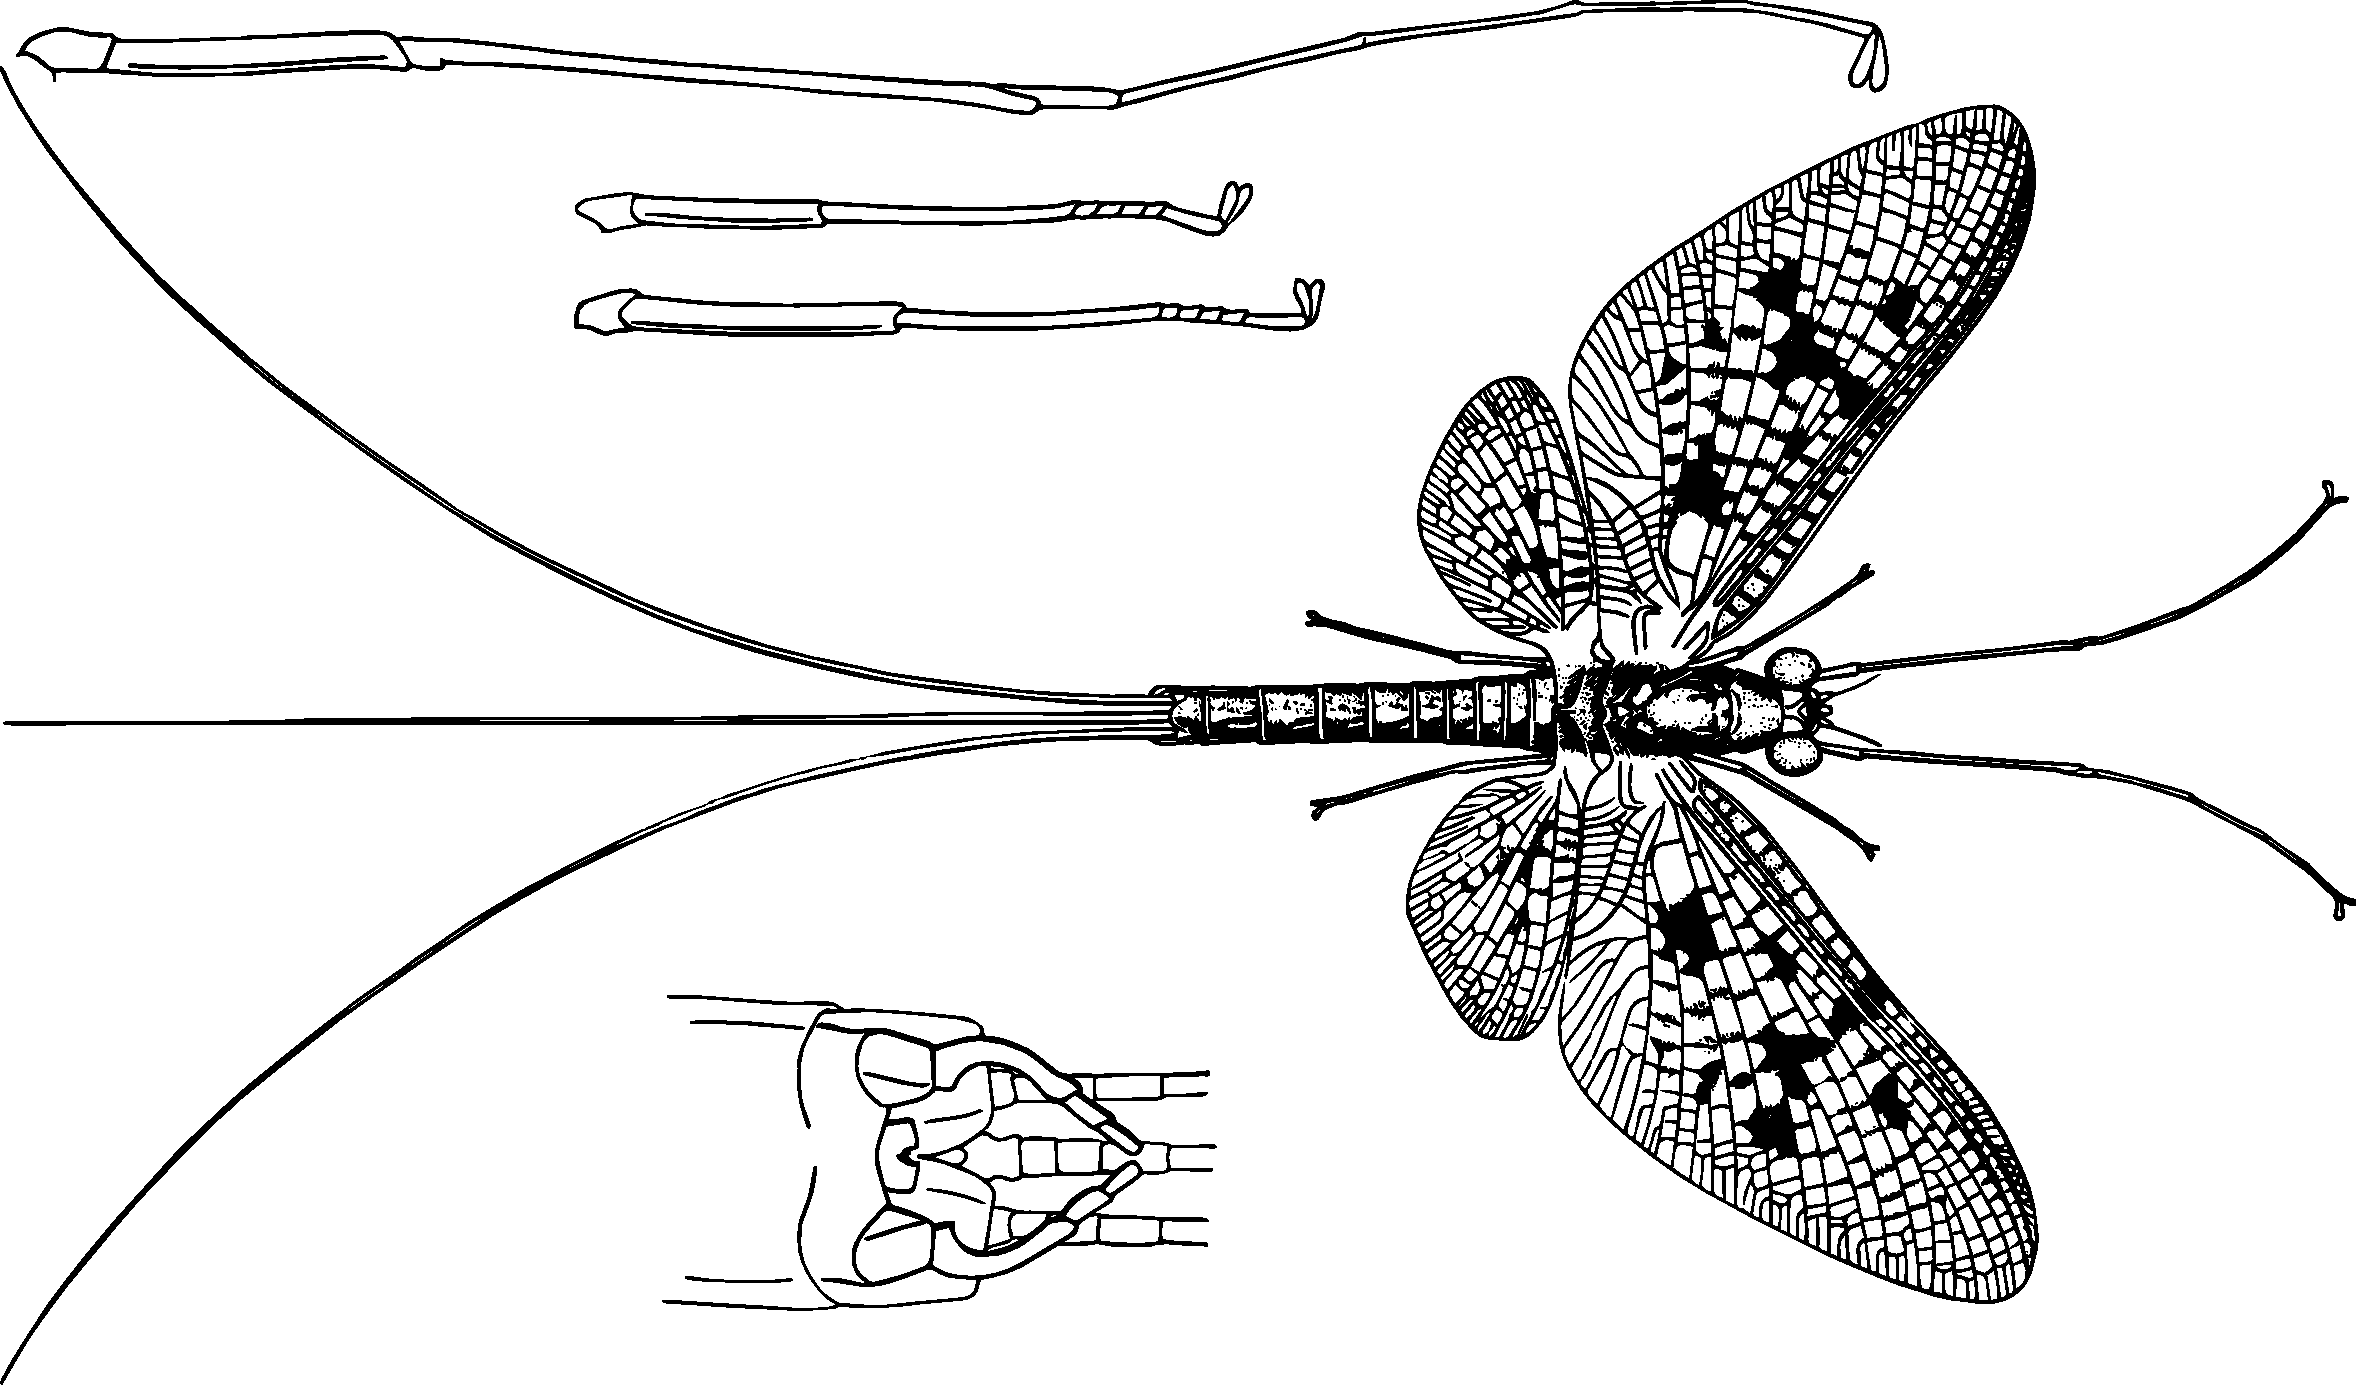
\includegraphics[width=0.8\textwidth]{paleoptera/Ephemeridae}
    \caption{Ephemeridae. \citep[modified from][Plate LXXV]{bhlitem81095ephem}}\label{fig:ephemerid}
\end{figure}

\subsubsection{Baetidae (minnow mayflies)}\index{Baetidae}
\noindent{}\textit{Diagnostic characters:} Adult small, usually \textless10 mm long; male compound eye turbinate (figure \ref{fig:baetid2}); cubital intercalaries (between CuA and CuP) in fore wing not present as 2 parallel pairs; \texorpdfstring{MP\textsubscript{2}}{ }{ }of fore wing not sharply angled towards Cu proximally; hind wing small or absent; hind leg tarsus with 4 tarsomeres; apex of abdomen with 2 long appendages.\vspace{3mm}

\noindent{}\textit{Natural history:} Naiads have streamlined shape, adapted for swimming in the water. They feed primarily on algae. There are approximately 1,000 described spp. worldwide.\vspace{3mm}

\begin{figure}[ht!]
    \centering
    \begin{subfigure}[ht!]{0.42\textwidth}
        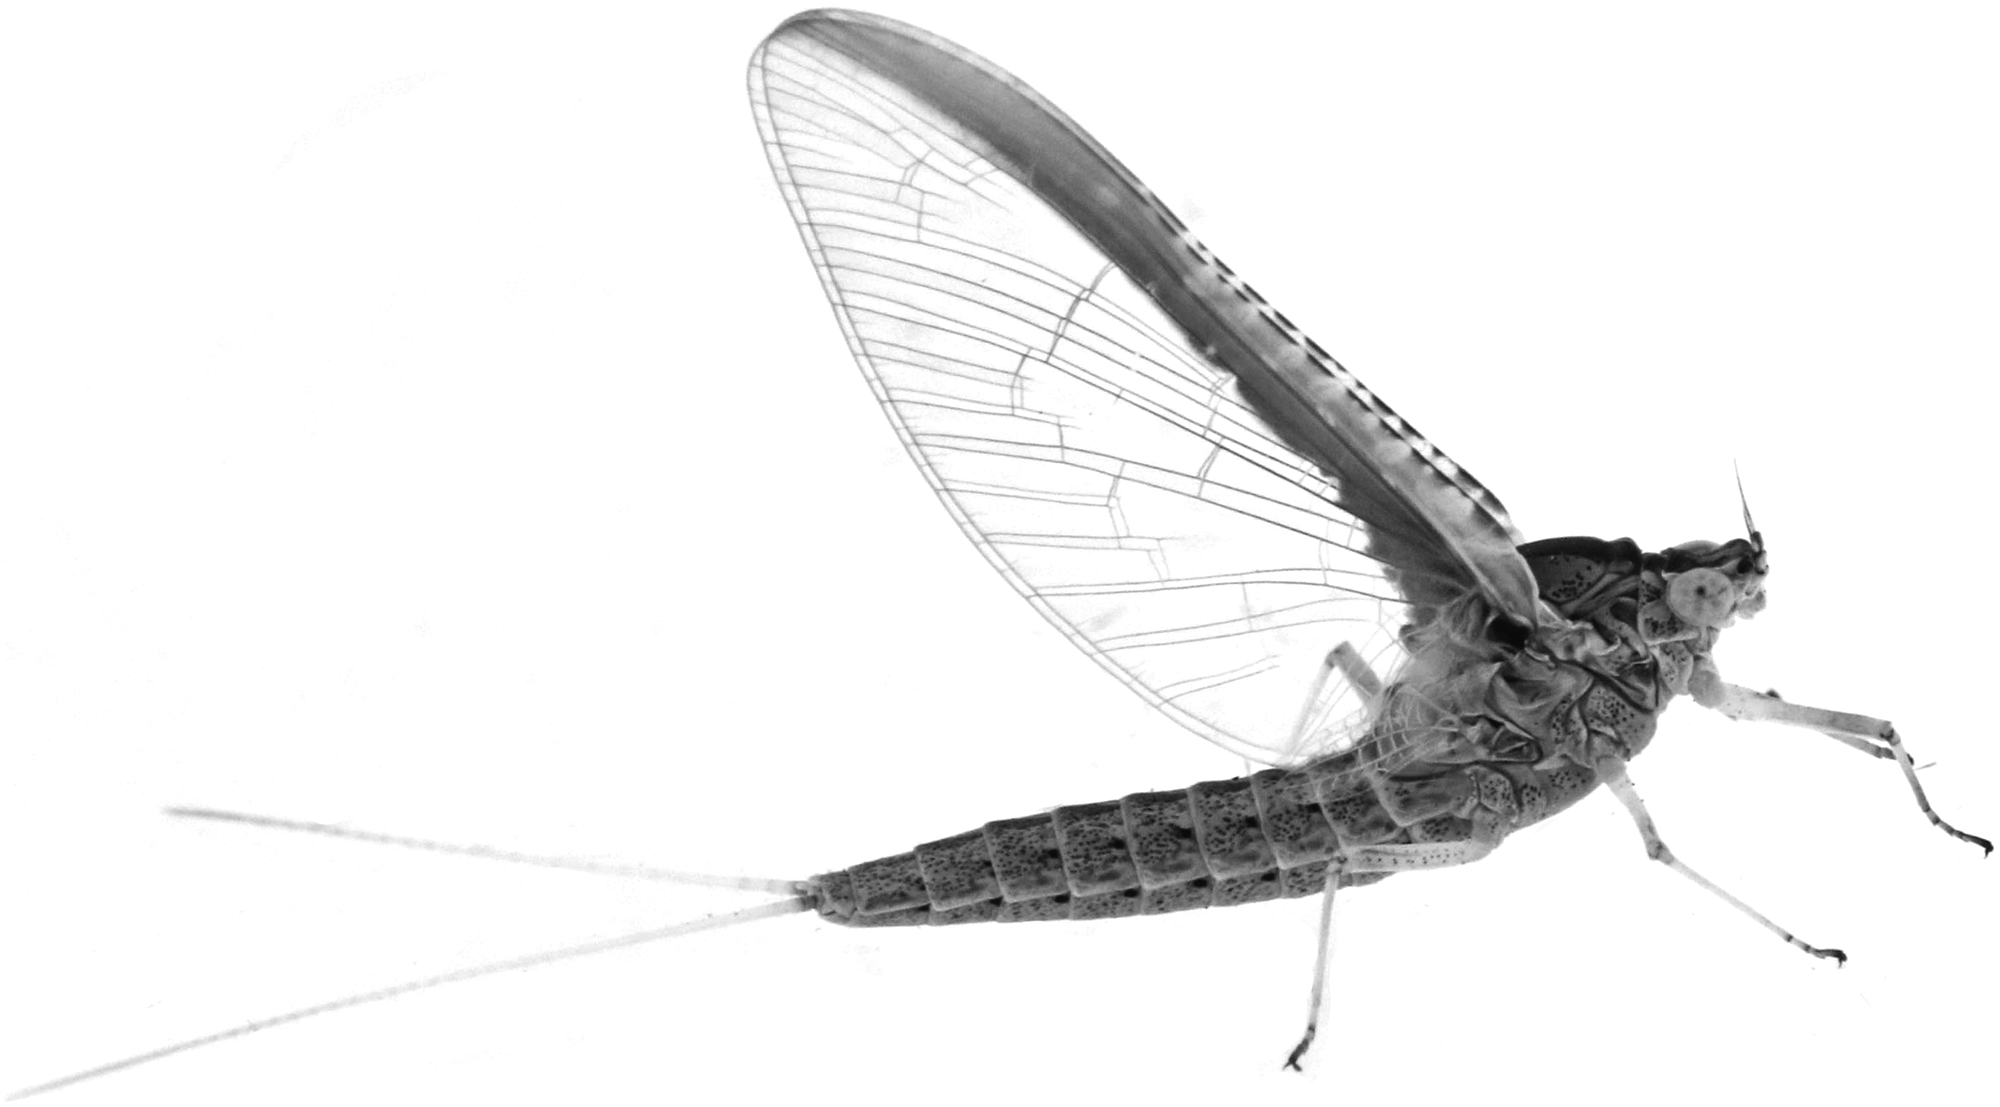
\includegraphics[width=\textwidth]{paleoptera/BaetidaeFemHabitus}
        \caption{}
        \label{fig:baetid1}
    \end{subfigure}
    \hfill
    \begin{subfigure}[ht!]{0.45\textwidth}
        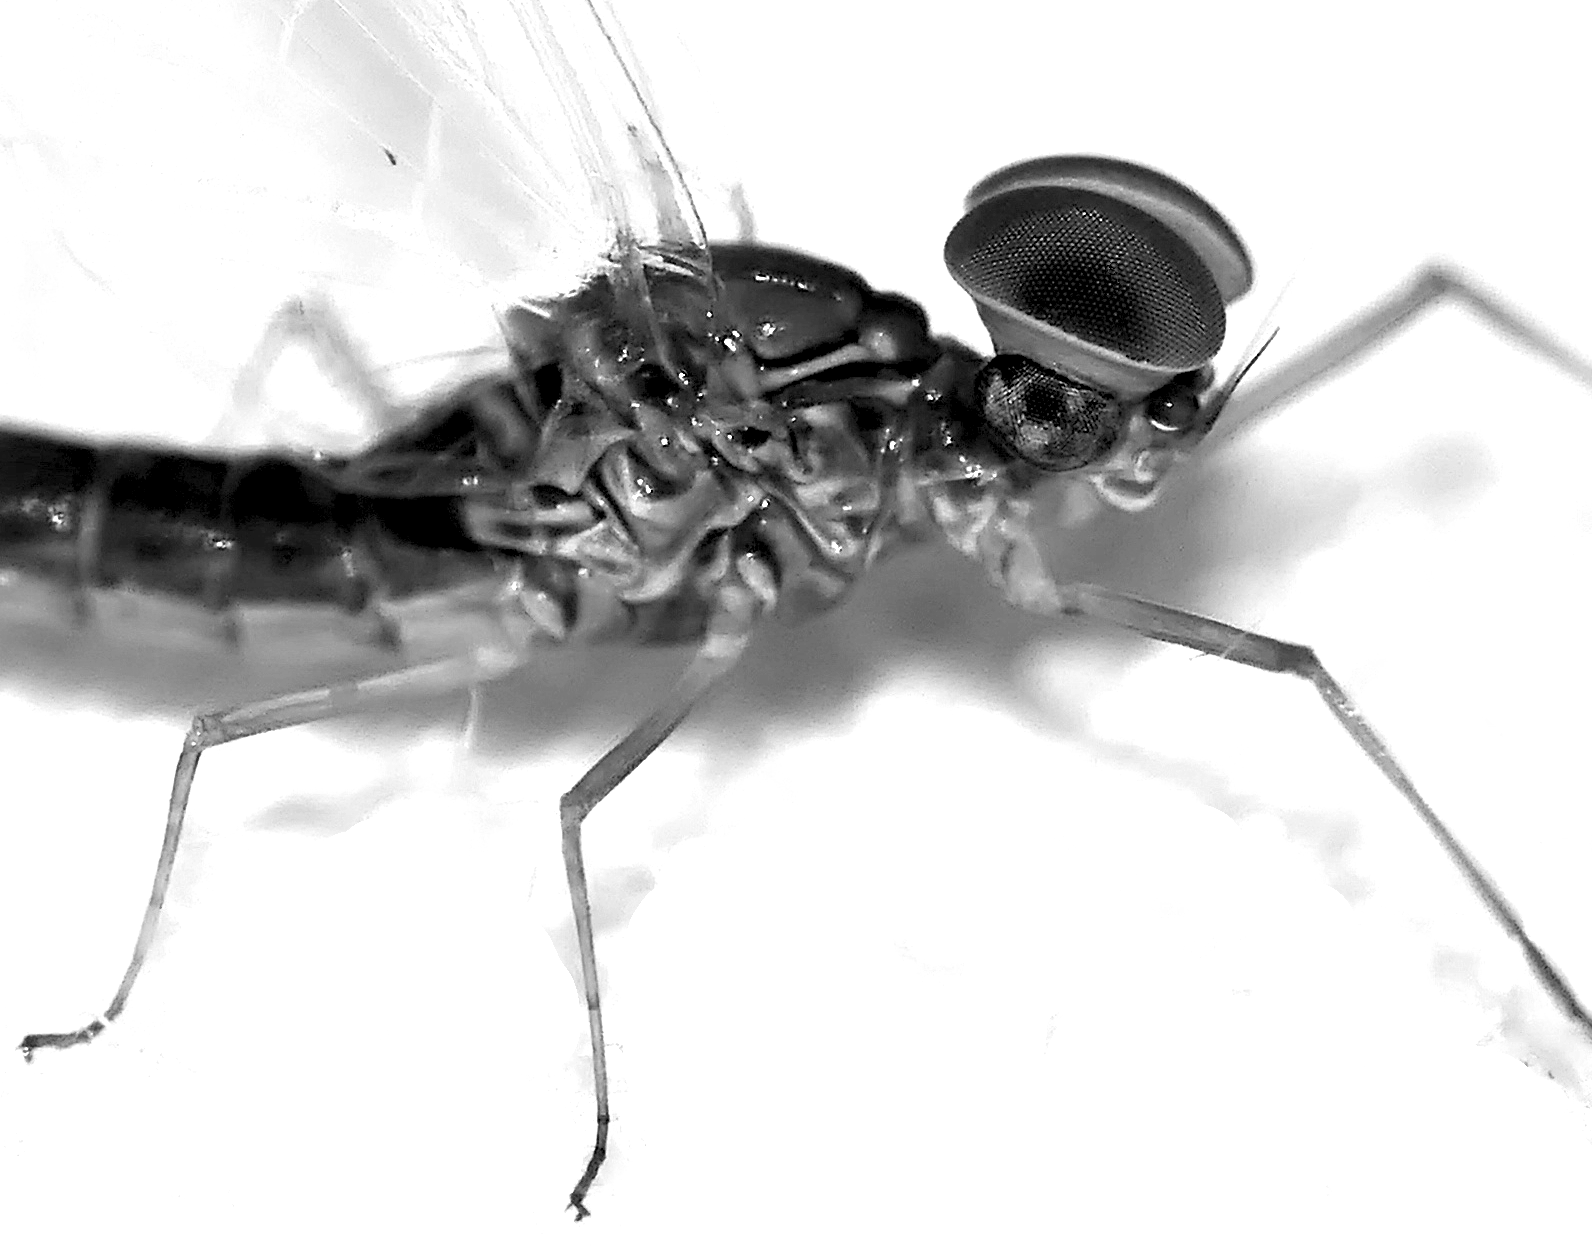
\includegraphics[width=\textwidth]{paleoptera/BaetidaeMaleHabitus}
        \caption{}
        \label{fig:baetid2}
    \end{subfigure}
    \caption{Baetidae. \textbf{(a)} Female habitus, photo (CC BY 2.0) by Andrey Zharkikh \url{https://flic.kr/p/AnyRSm}; \textbf{(b)} Male habitus, not conspecific with \ref{fig:baetid1}, photo (CC BY-SA 2.0) by Bernard DuPont \url{https://flic.kr/p/Ru6AuY}}\label{fig:baetids}
\end{figure}

\subsubsection{Heptageniidae (flat-headed mayflies, stream mayflies)}\index{Heptageniidae}
\noindent{}\textit{Diagnostic characters:} Adult size variable; male compound eye round, unmodified; cubital intercalaries (between CuA and CuP) in fore wing present as 2 parallel pairs; \texorpdfstring{MP\textsubscript{2}}{ }{ }of fore wing not sharply angled towards Cu proximally; hind wing large, visible, with many veins; hind leg tarsus with 5 tarsomeres; apex of abdomen with 2 long appendages.\vspace{3mm}

\noindent{}\textit{Natural history:} Naiads have flattened shape, adapted for living in the boundary layer in lotic systems. They have diverse feeding habits, with many species scraping algae, while others scavenge or predate on other invertebrates. There are approximately 500 described spp. worldwide.\vspace{3mm}

\begin{figure}[ht!]
    \centering
    \begin{subfigure}[ht!]{0.5\textwidth}
        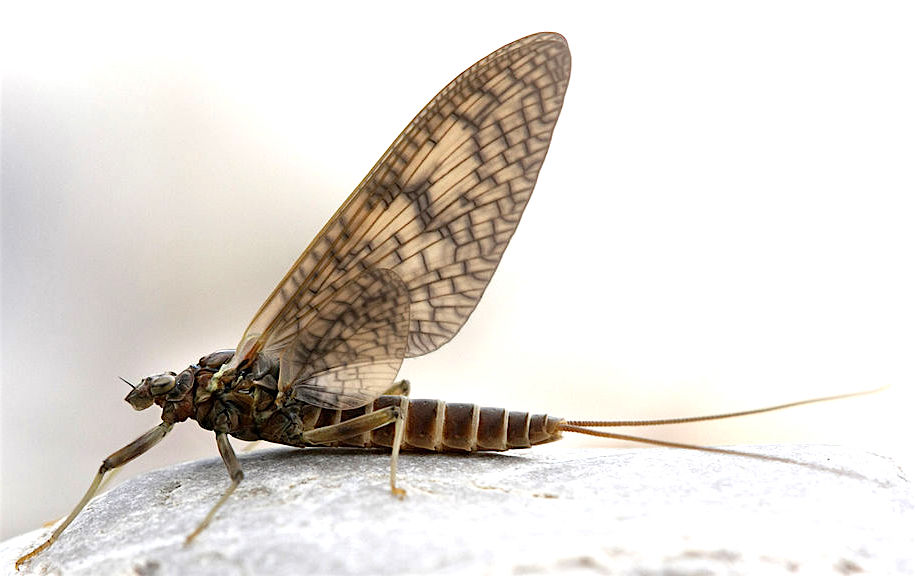
\includegraphics[width=\textwidth]{paleoptera/HeptageniidHabitus}
        \caption{}
        \label{fig:heptageniid1}
    \end{subfigure}
    \hfill
    \begin{subfigure}[ht!]{0.4\textwidth}
        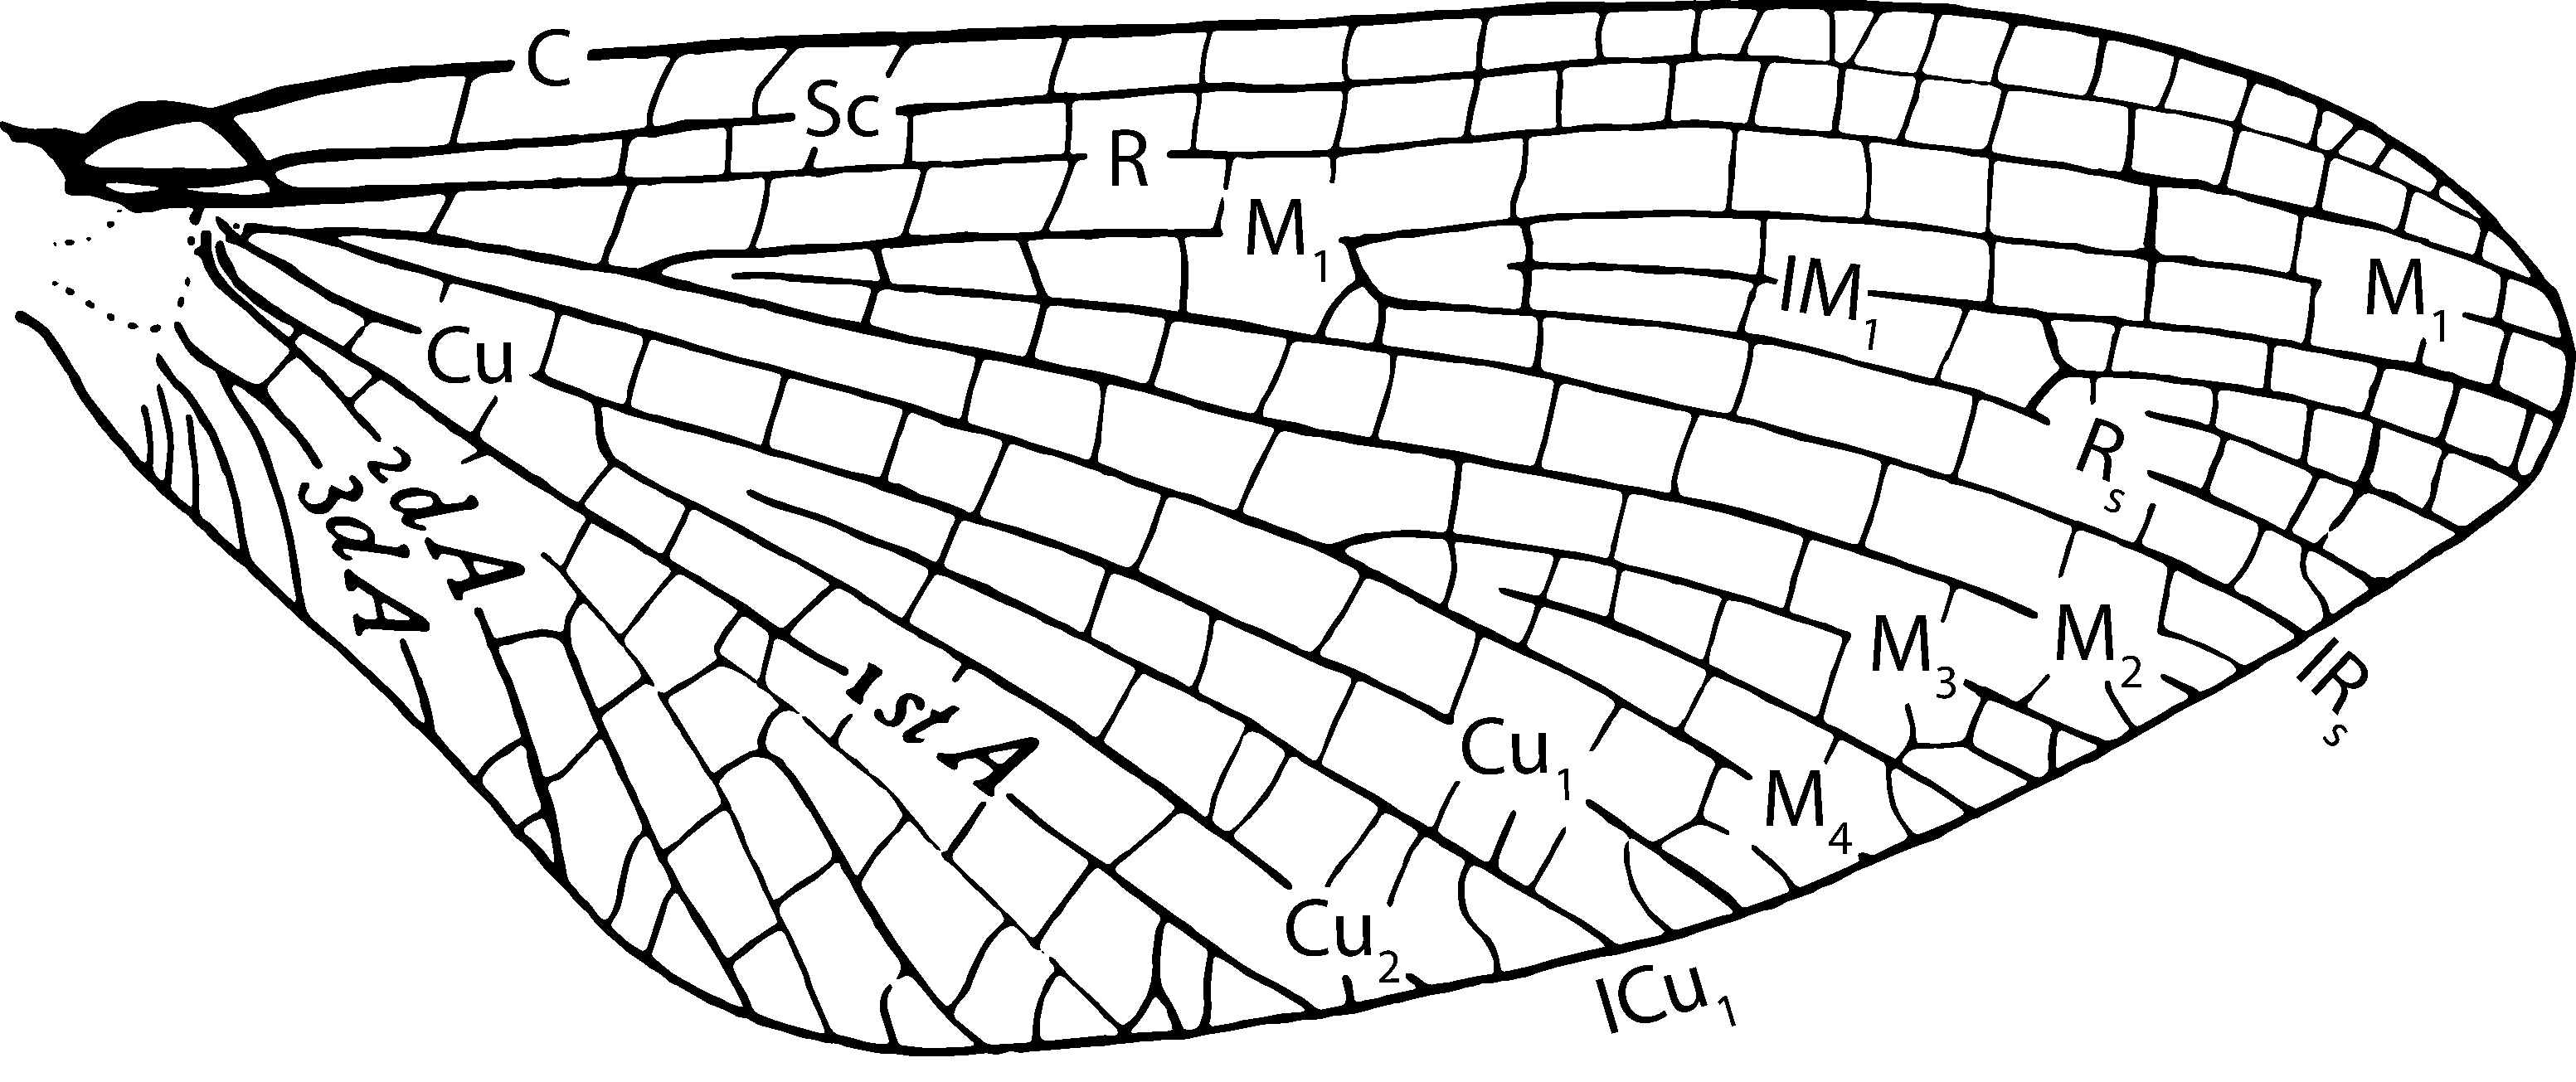
\includegraphics[width=\textwidth]{paleoptera/HeptageniidWing}
        \caption{}
        \label{fig:heptageniid2}
    \end{subfigure}
    \caption{Heptageniidae. \textbf{(a)} Habitus, drawn from photo (CC BY-SA) by Richard Bartz \url{https://commons.wikimedia.org/wiki/File:Ephemeroptera_2.jpg}; \textbf{(b)} fore wing venation \citep[redrawn from][Fig. 61]{comstock1918wings}}\label{fig:heptageniid}
\end{figure}

\FloatBarrier

\section{Odonata (dragonflies, damselflies)}\index{Odonata}
Like their putative sister lineage, Ephemeroptera, immature Odonata are almost exclusively aquatic. All species are predaceous in all stages, with adaptations that facilitate prey tracking, stalking, and capture.\vspace{3mm}%add naiads and adults diag chars?

\begin{theo}
{}Can you list at least three adaptations you see across Odonata families that you hypothesize facilitate predation?\\

\noindent{}Odonata adults are prepared using an unorthodox approach, relative to other Pterygota (see Section \ref{odeprep}). Why?\index[preps]{Odonata}
\end{theo}\vspace{3mm}

\noindent{}Another conspicuous synapomorphy for Odonata is the evolution of a secondary copulatory organ ventrally on the first abdominal segment of males. Females are grabbed and held behind the head by the male, using his apical abdominal appendages. Be sure to look for adaptations associated with this unusual copulatory habit.\vspace{3mm}

\begin{theo}
{}Sketch a feature on the female head that you suspect is an adaptation for this kind of copulation. How do you think the secondary male genitalia evolved? What did the early, intermediate form look like?
\end{theo}\vspace{3mm}

\noindent{}Odonata is the first group where each wing has a distinct pterostigma (pigmented spot on anterior edge of wing). The pterostigma is not only highly pigmented but also more sclerotized and more massive than other wing areas.\vspace{3mm}

\subsection{Anisoptera (dragonflies)}

\subsubsection{Gomphidae (clubtails)}\index{Gomphidae}
\noindent{}\textit{Diagnostic characters:} Compound eyes separated dorsally, triangular wing cells (``triangles'') in fore wing and hind wing similar in shape and location, apical abdominal segments often expanded laterally, forming a ``club''.\vspace{3mm}

\noindent{}\textit{Natural history:} Larvae are usually found in lotic systems, where they bury themselves in the substrate and wait for prey. Look for adults on flat perches, \textit{e.g.}, on the ground or on leaves. Approximately 900 spp. have been described worldwide.\vspace{3mm}

\begin{figure}[ht!]
    \centering
    \begin{subfigure}[ht!]{0.4\textwidth}
        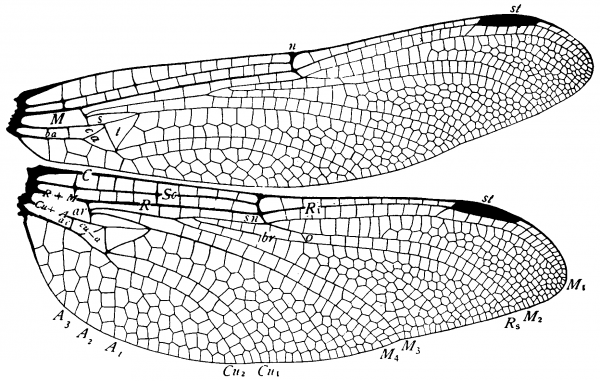
\includegraphics[width=\textwidth]{paleoptera/GomphidaeWing}
        \caption{}
        \label{fig:gomphid1}
    \end{subfigure}
    \hfill
    \begin{subfigure}[ht!]{0.55\textwidth}
        \reflectbox{
        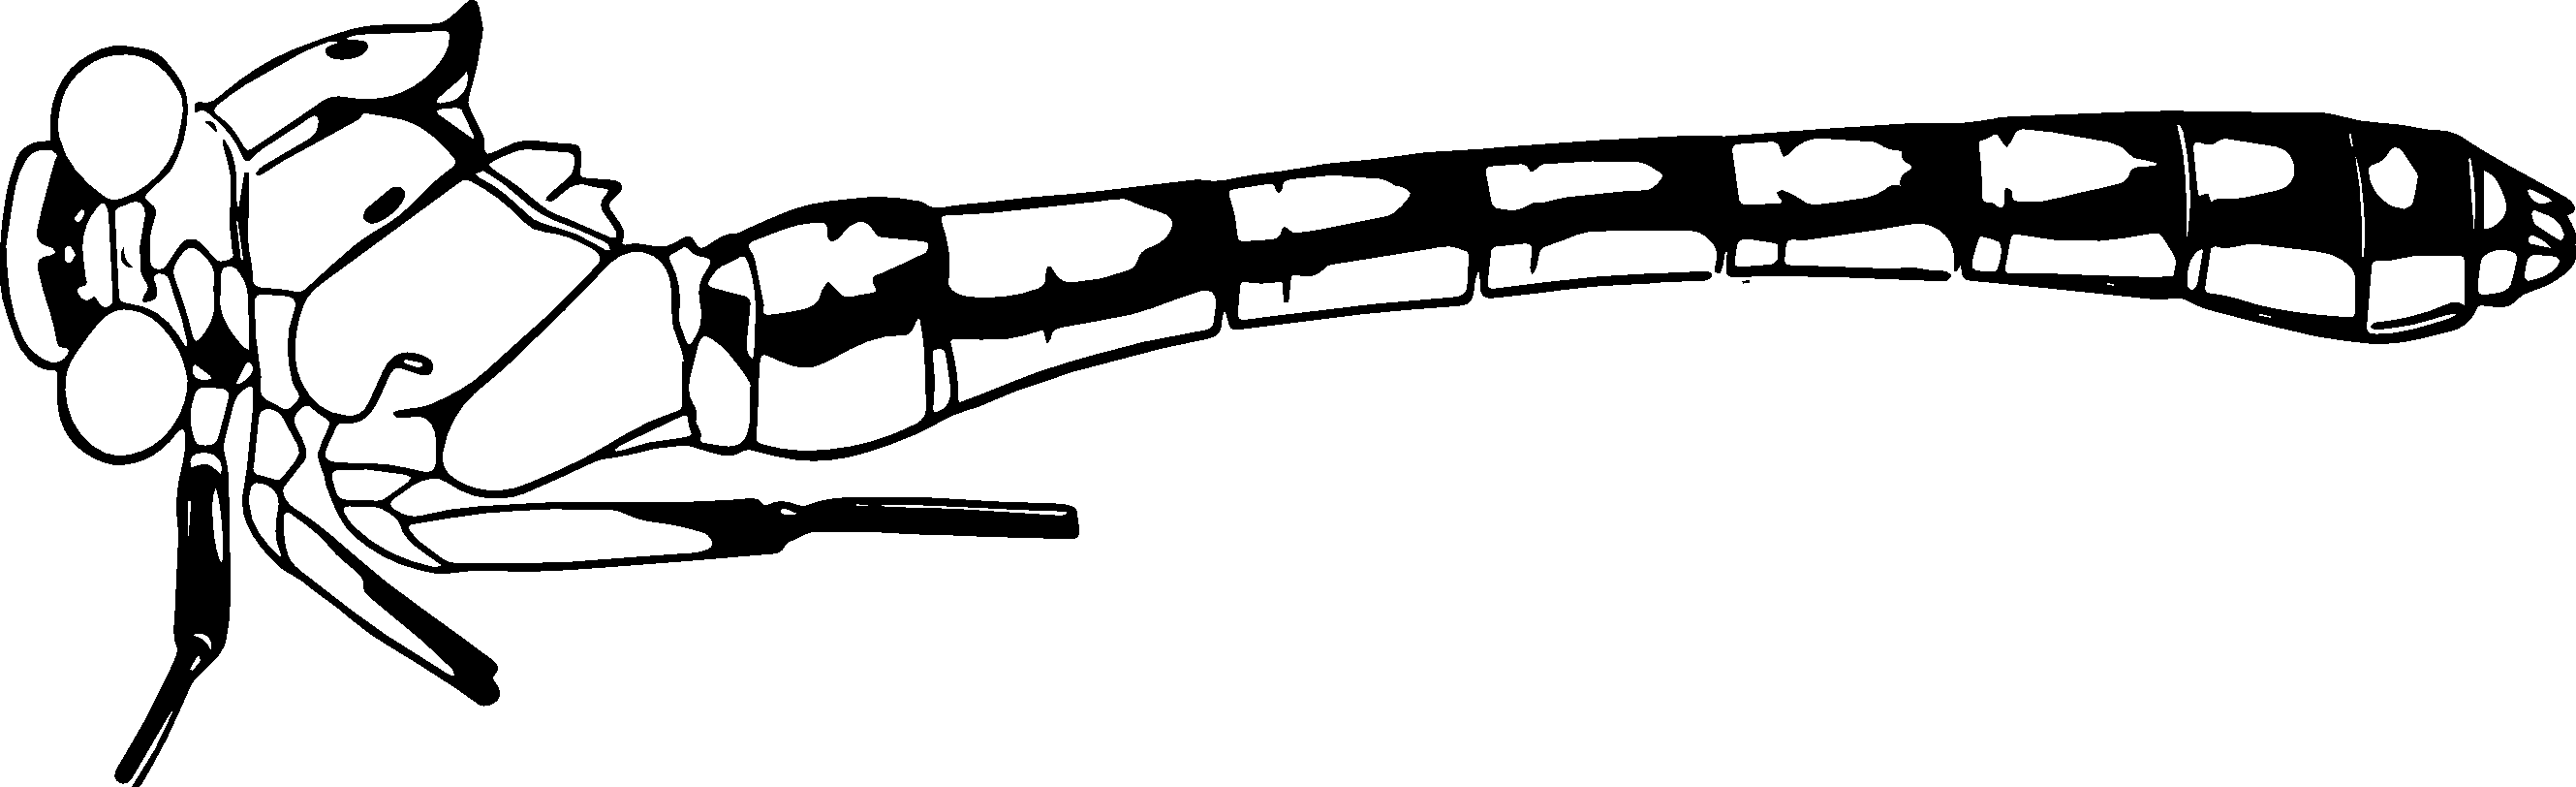
\includegraphics[width=\textwidth]{paleoptera/gomphidBody}}
        \caption{}
        \label{fig:gomphid2}
    \end{subfigure}
    \caption{Gomphidae. \textbf{(a)} Wing venation \citep[][Fig. 229]{comstock1918wings}; \textbf{(b)} head (twisted 90\textdegree), thorax, and abdomen \citep[redrawn from][Fig. 4:17 f1]{bhlitem126080aquatic}}\label{fig:gomphids} 
\end{figure}

\subsubsection{Aeshnidae (darners, hawkers)}\index{Aeshnidae}
\noindent{}\textit{Diagnostic characters:} Compound eyes adjacent dorsally, triangular wing areas (``triangles'') in fore wing and hind wing similar in shape and location, ovipositor well developed.\vspace{3mm}

\noindent{}\textit{Natural history:} Larvae are often thought of as being part of the ``climber'' guild of aquatic insects, as they are usually found in aquatic vegetation. Do they appear to be adapted for climbing and hunting in vegetation (see figure \ref{fig:OdonataLarva})? Adults are typically large and are very strong fliers. One can find these dragonflies in/near almost any aquatic habitat. Approximately 440 spp. have been described worldwide.\vspace{3mm}

\begin{figure}[ht!]
    \centering
    \begin{subfigure}[ht!]{0.48\textwidth}
        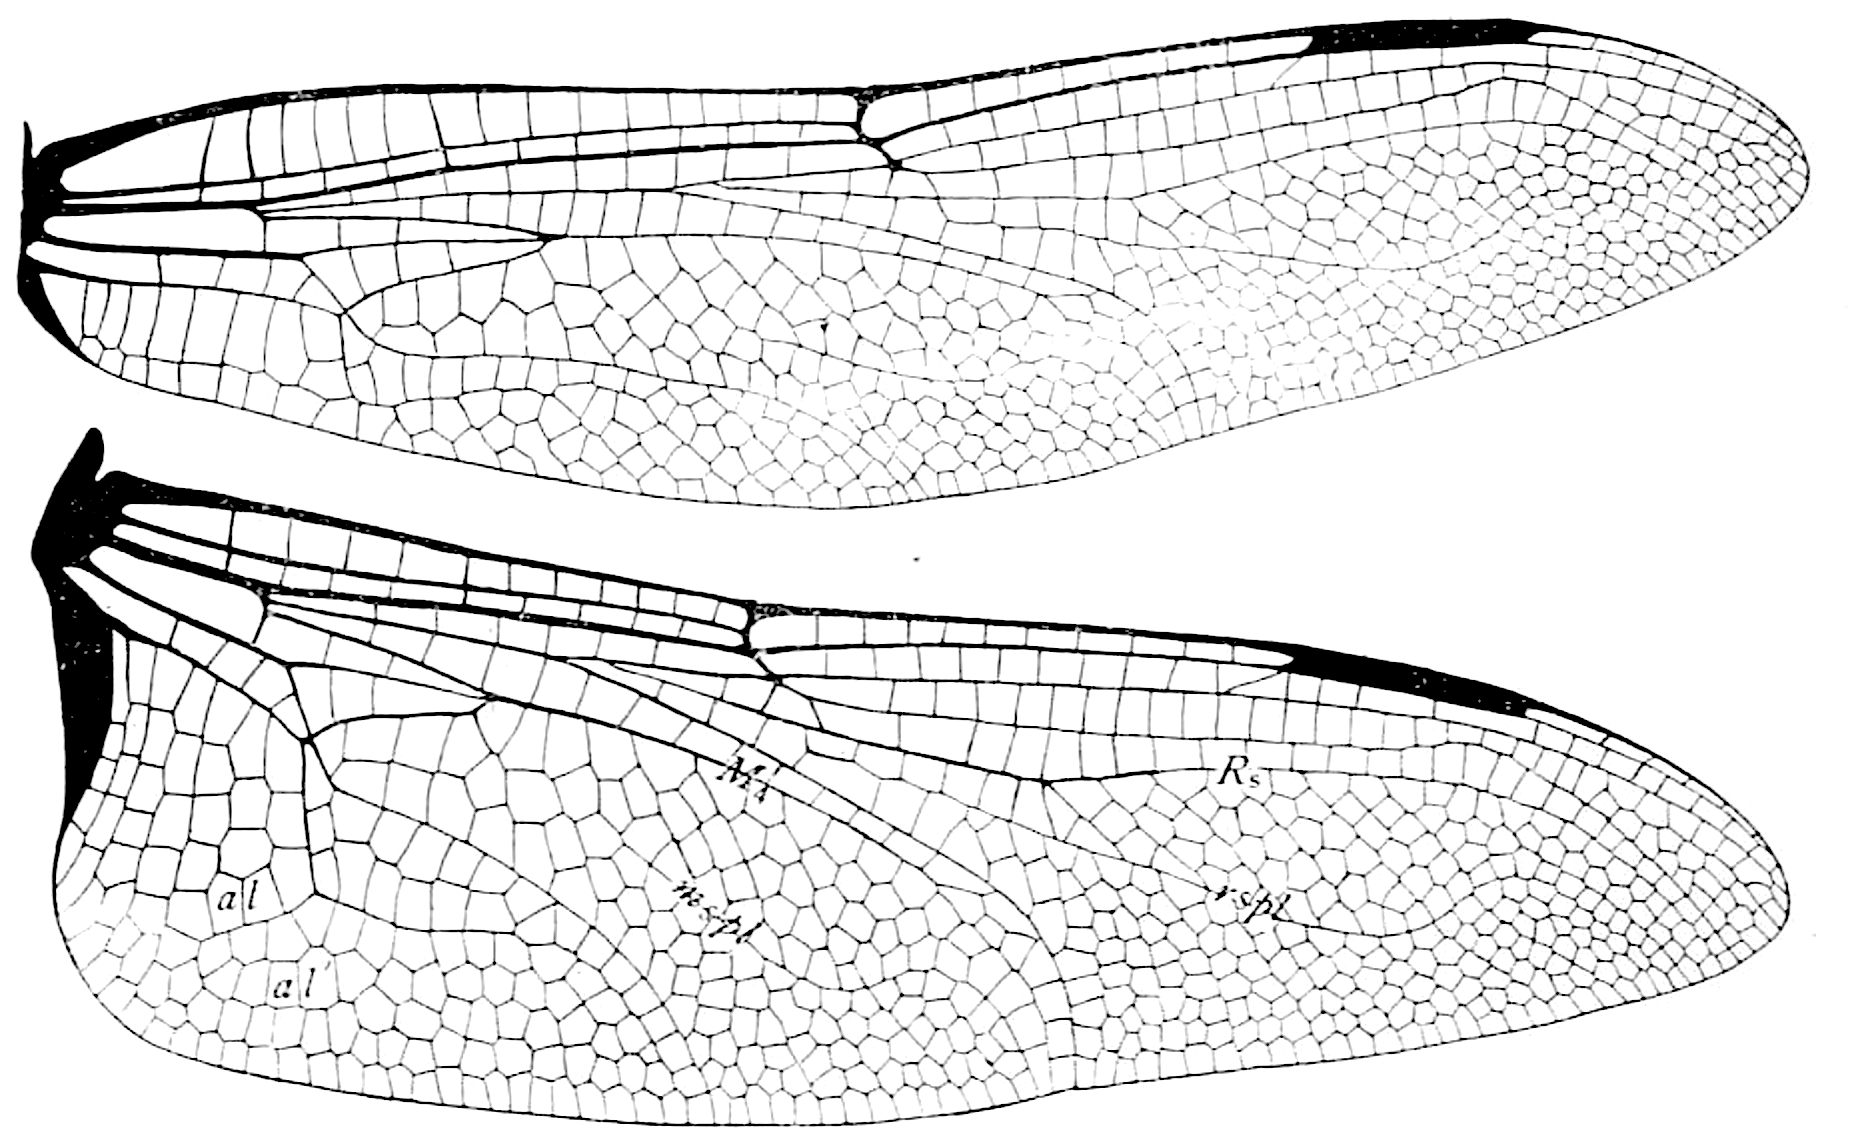
\includegraphics[width=\textwidth]{paleoptera/AeshnidWings}
        \caption{}
        \label{fig:aeshnid1}
    \end{subfigure}
    \hfill
    \begin{subfigure}[ht!]{0.3\textwidth}
        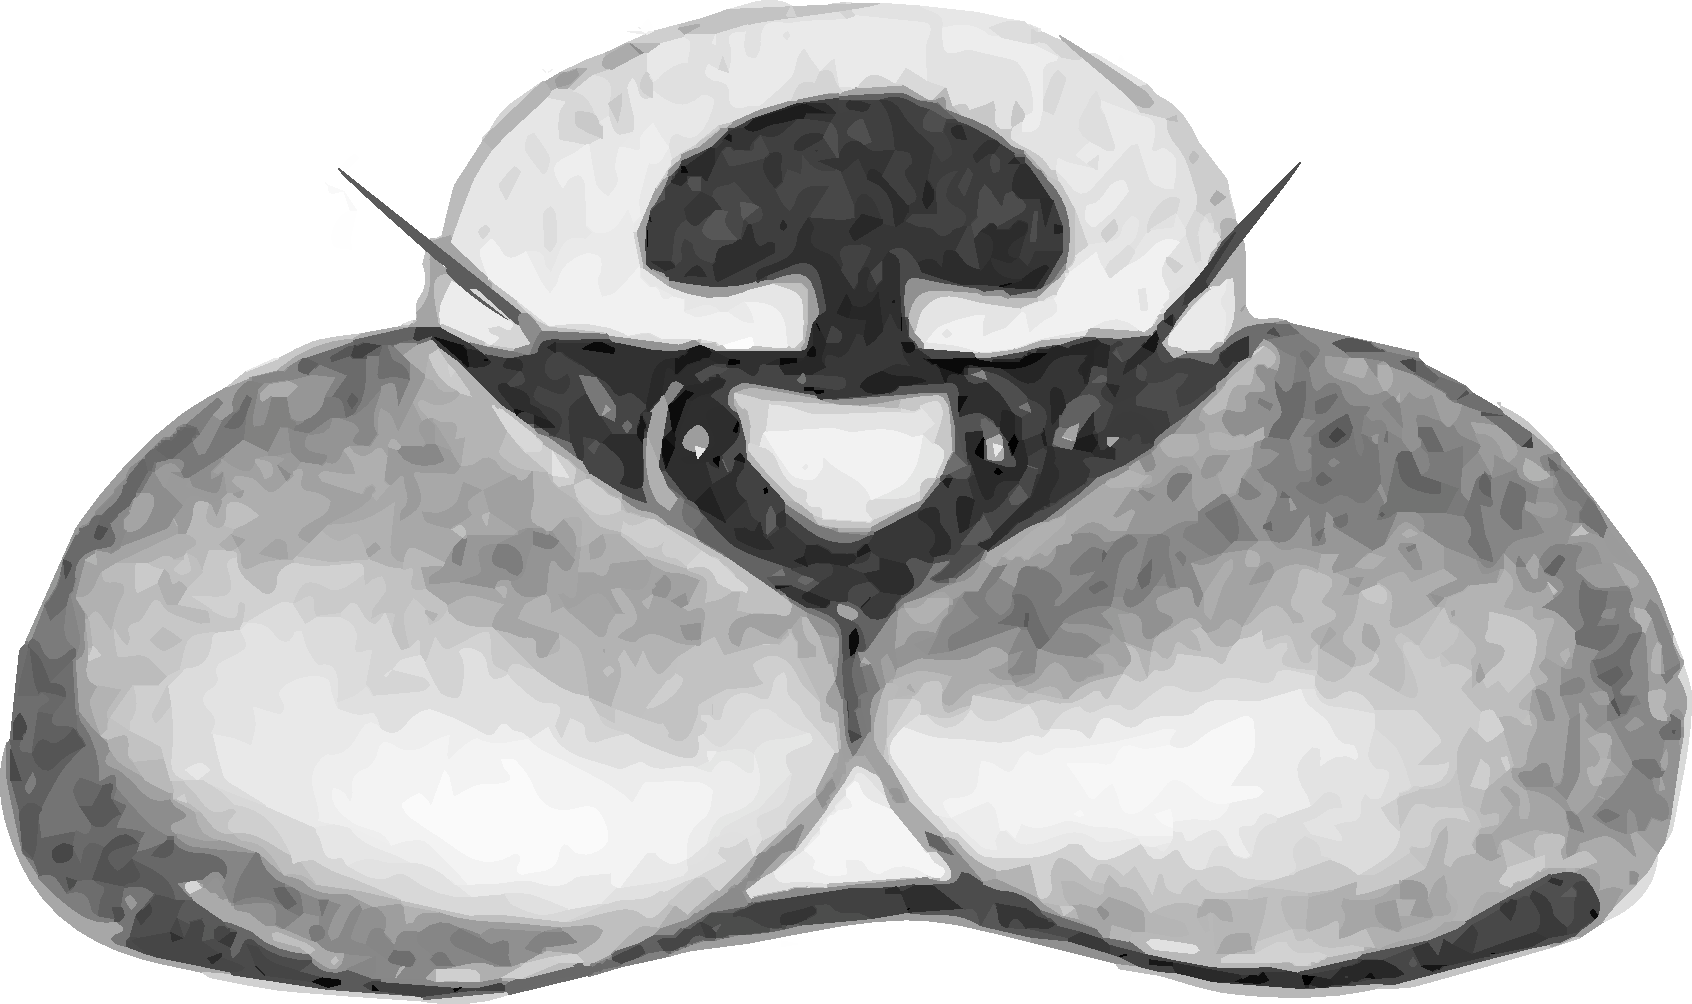
\includegraphics[width=\textwidth]{paleoptera/aeshnidHead}
        \caption{}
        \label{fig:aeshnid2}
    \end{subfigure}
    \caption{Aeshnidae. \textbf{(a)} Wing venation \citep[][Fig. 236]{comstock1918wings}; \textbf{(b)} head in dorsal view \citep[][Plate 22, Fig. 3]{aeshnaNorthAmerica}}\label{fig:aeshnids}
\end{figure}

\begin{figure}[ht!]
  \centering
    \reflectbox{%
    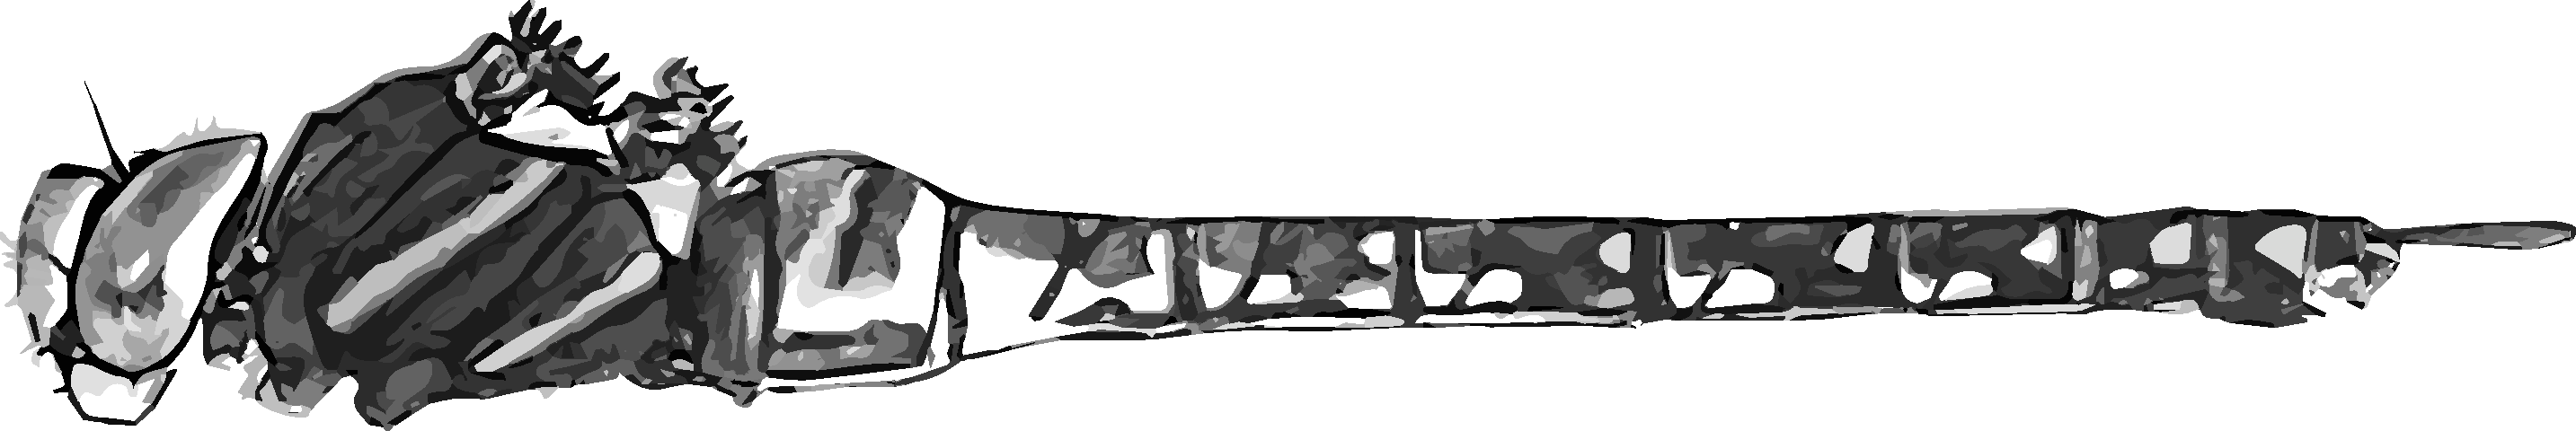
\includegraphics[width=0.7\textwidth]{paleoptera/aeshnidHabitus}}
  \caption{Aeshnidae lateral habitus \citep[][Plate 28, Fig. 5]{aeshnaNorthAmerica}}
  \label{fig:aeshnidHabitus}
\end{figure}

\subsubsection{Libellulidae (common skimmers)} \index{Libellulidae}
\noindent{}\textit{Diagnostic characters:} Compound eyes meeting dorsally, triangles in fore wing and hind wing different in shape, hind wing with boot-shaped area, ovipositor absent.\vspace{3mm}

\noindent{}\textit{Natural history:} Larvae are usually thought of as ``sprawlers'', which generally sit relatively still on the bottom, in the sediment, waiting for prey. Can you see major morphological differences between these larvae and other odonates? Adults are diverse in size, color, and habitat. More than 1,000 spp. have been described worldwide.\vspace{3mm}

\begin{figure}[ht!]
    \centering
    \begin{subfigure}[ht!]{0.5\textwidth}
        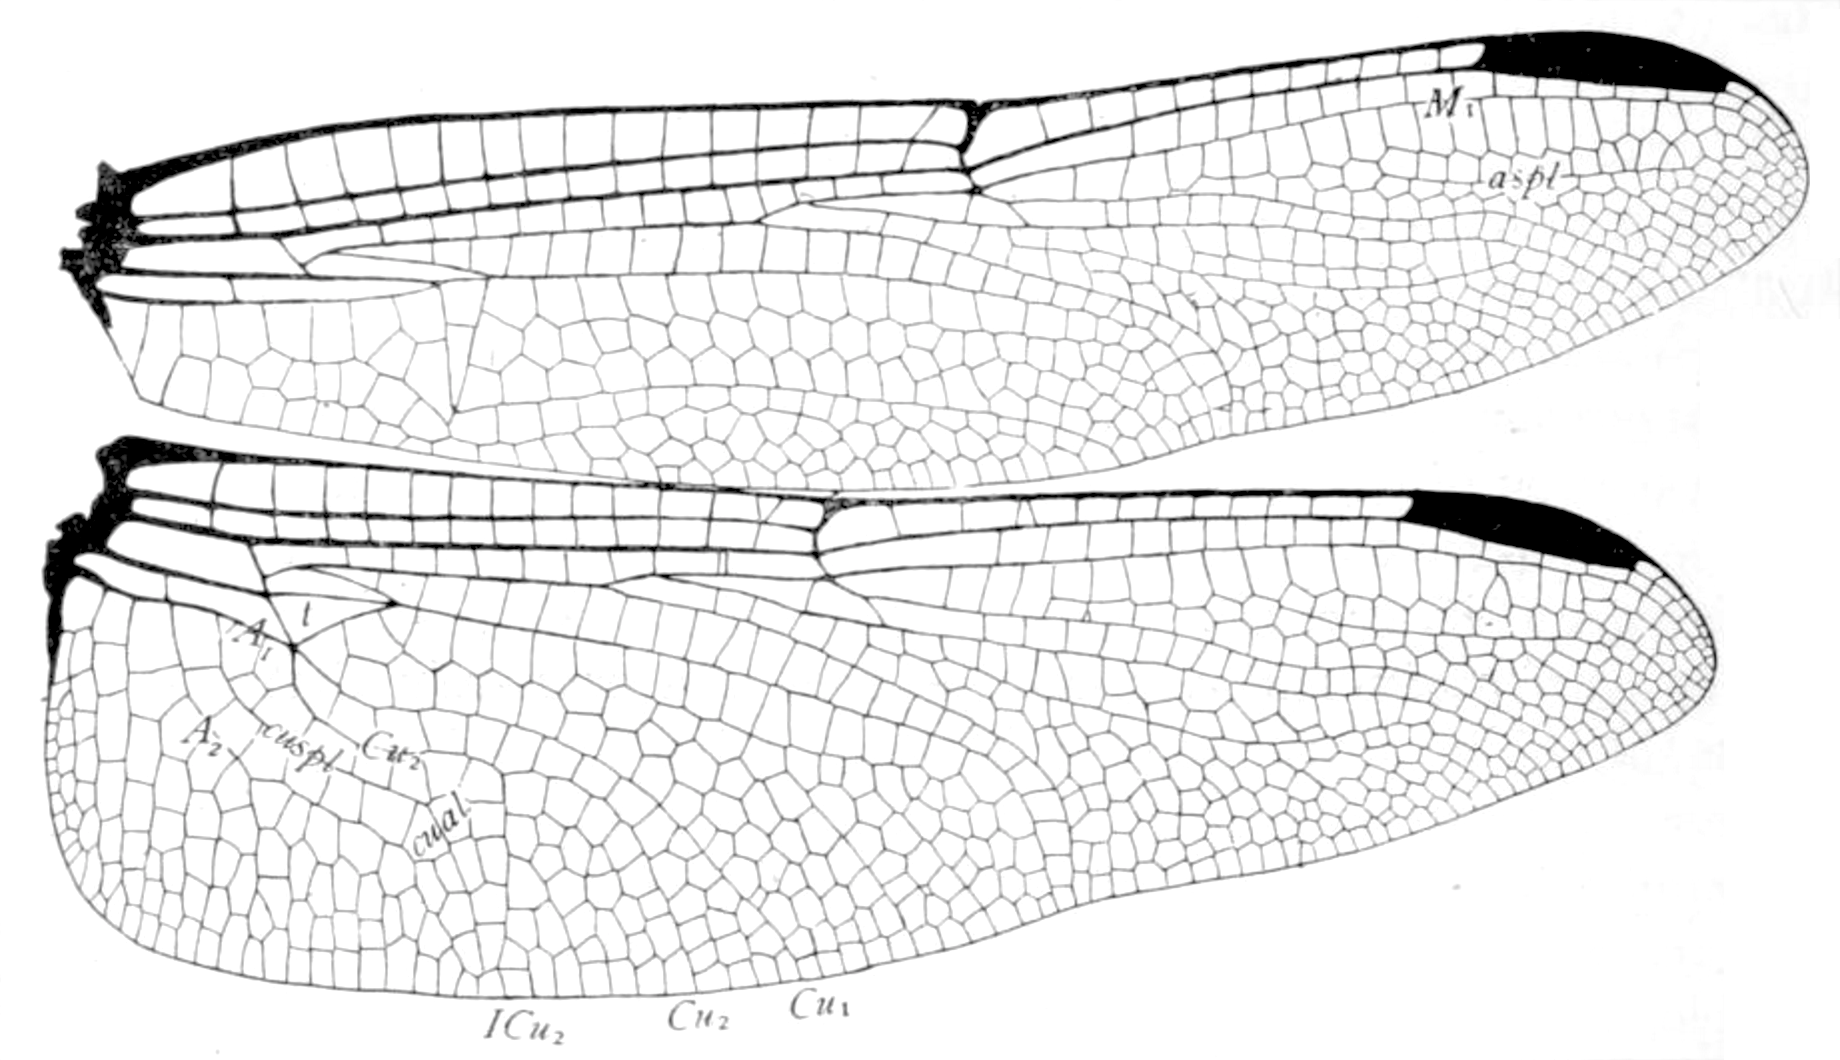
\includegraphics[width=\textwidth]{paleoptera/LibellulidWings}
        \caption{}
        \label{fig:libelwing}
    \end{subfigure}
    \hfill
    \begin{subfigure}[ht!]{0.25\textwidth}
        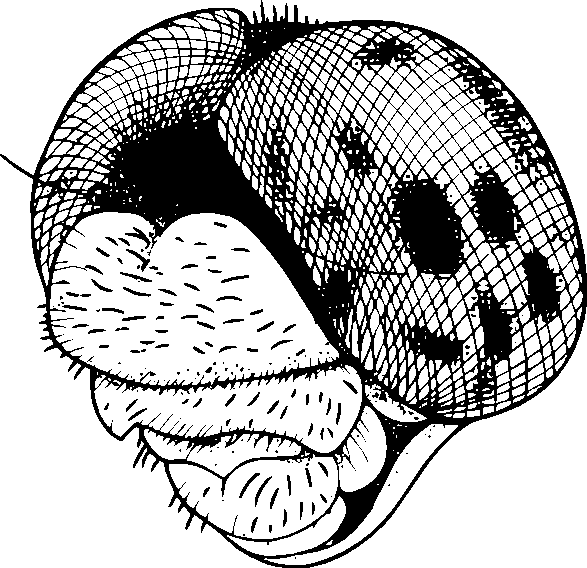
\includegraphics[width=\textwidth]{paleoptera/LibellulidaeHead}
        \caption{}
        \label{fig:libelbody}
    \end{subfigure}
    \caption{Libellulidae. \textbf{(a)} Wing venation \citep[][Fig. 240]{comstock1918wings}; \textbf{(b)} head (illustration by Laura Porturas, Penn State)}\label{fig:libell}
\end{figure}

\subsection{Zygoptera (damselflies)}
\subsubsection{Calopterygidae (jewelwings, broad-winged damselflies)}\index{Calopterygidae}
\noindent{}\textit{Diagnostic characters:} Wings tapered at base, numerous antenodal crossveins present (proximal to nodus).\vspace{3mm}

\noindent{}\textit{Natural history:} Like other damselflies, larvae are usually thought of as climbers. Larvae and adults are usually found along streams (\textit{i.e.}, lotic systems). Approximately 150 spp. have been described worldwide.\vspace{3mm}

\begin{figure}[ht!]
    \centering
    \begin{subfigure}[ht!]{0.45\textwidth}
        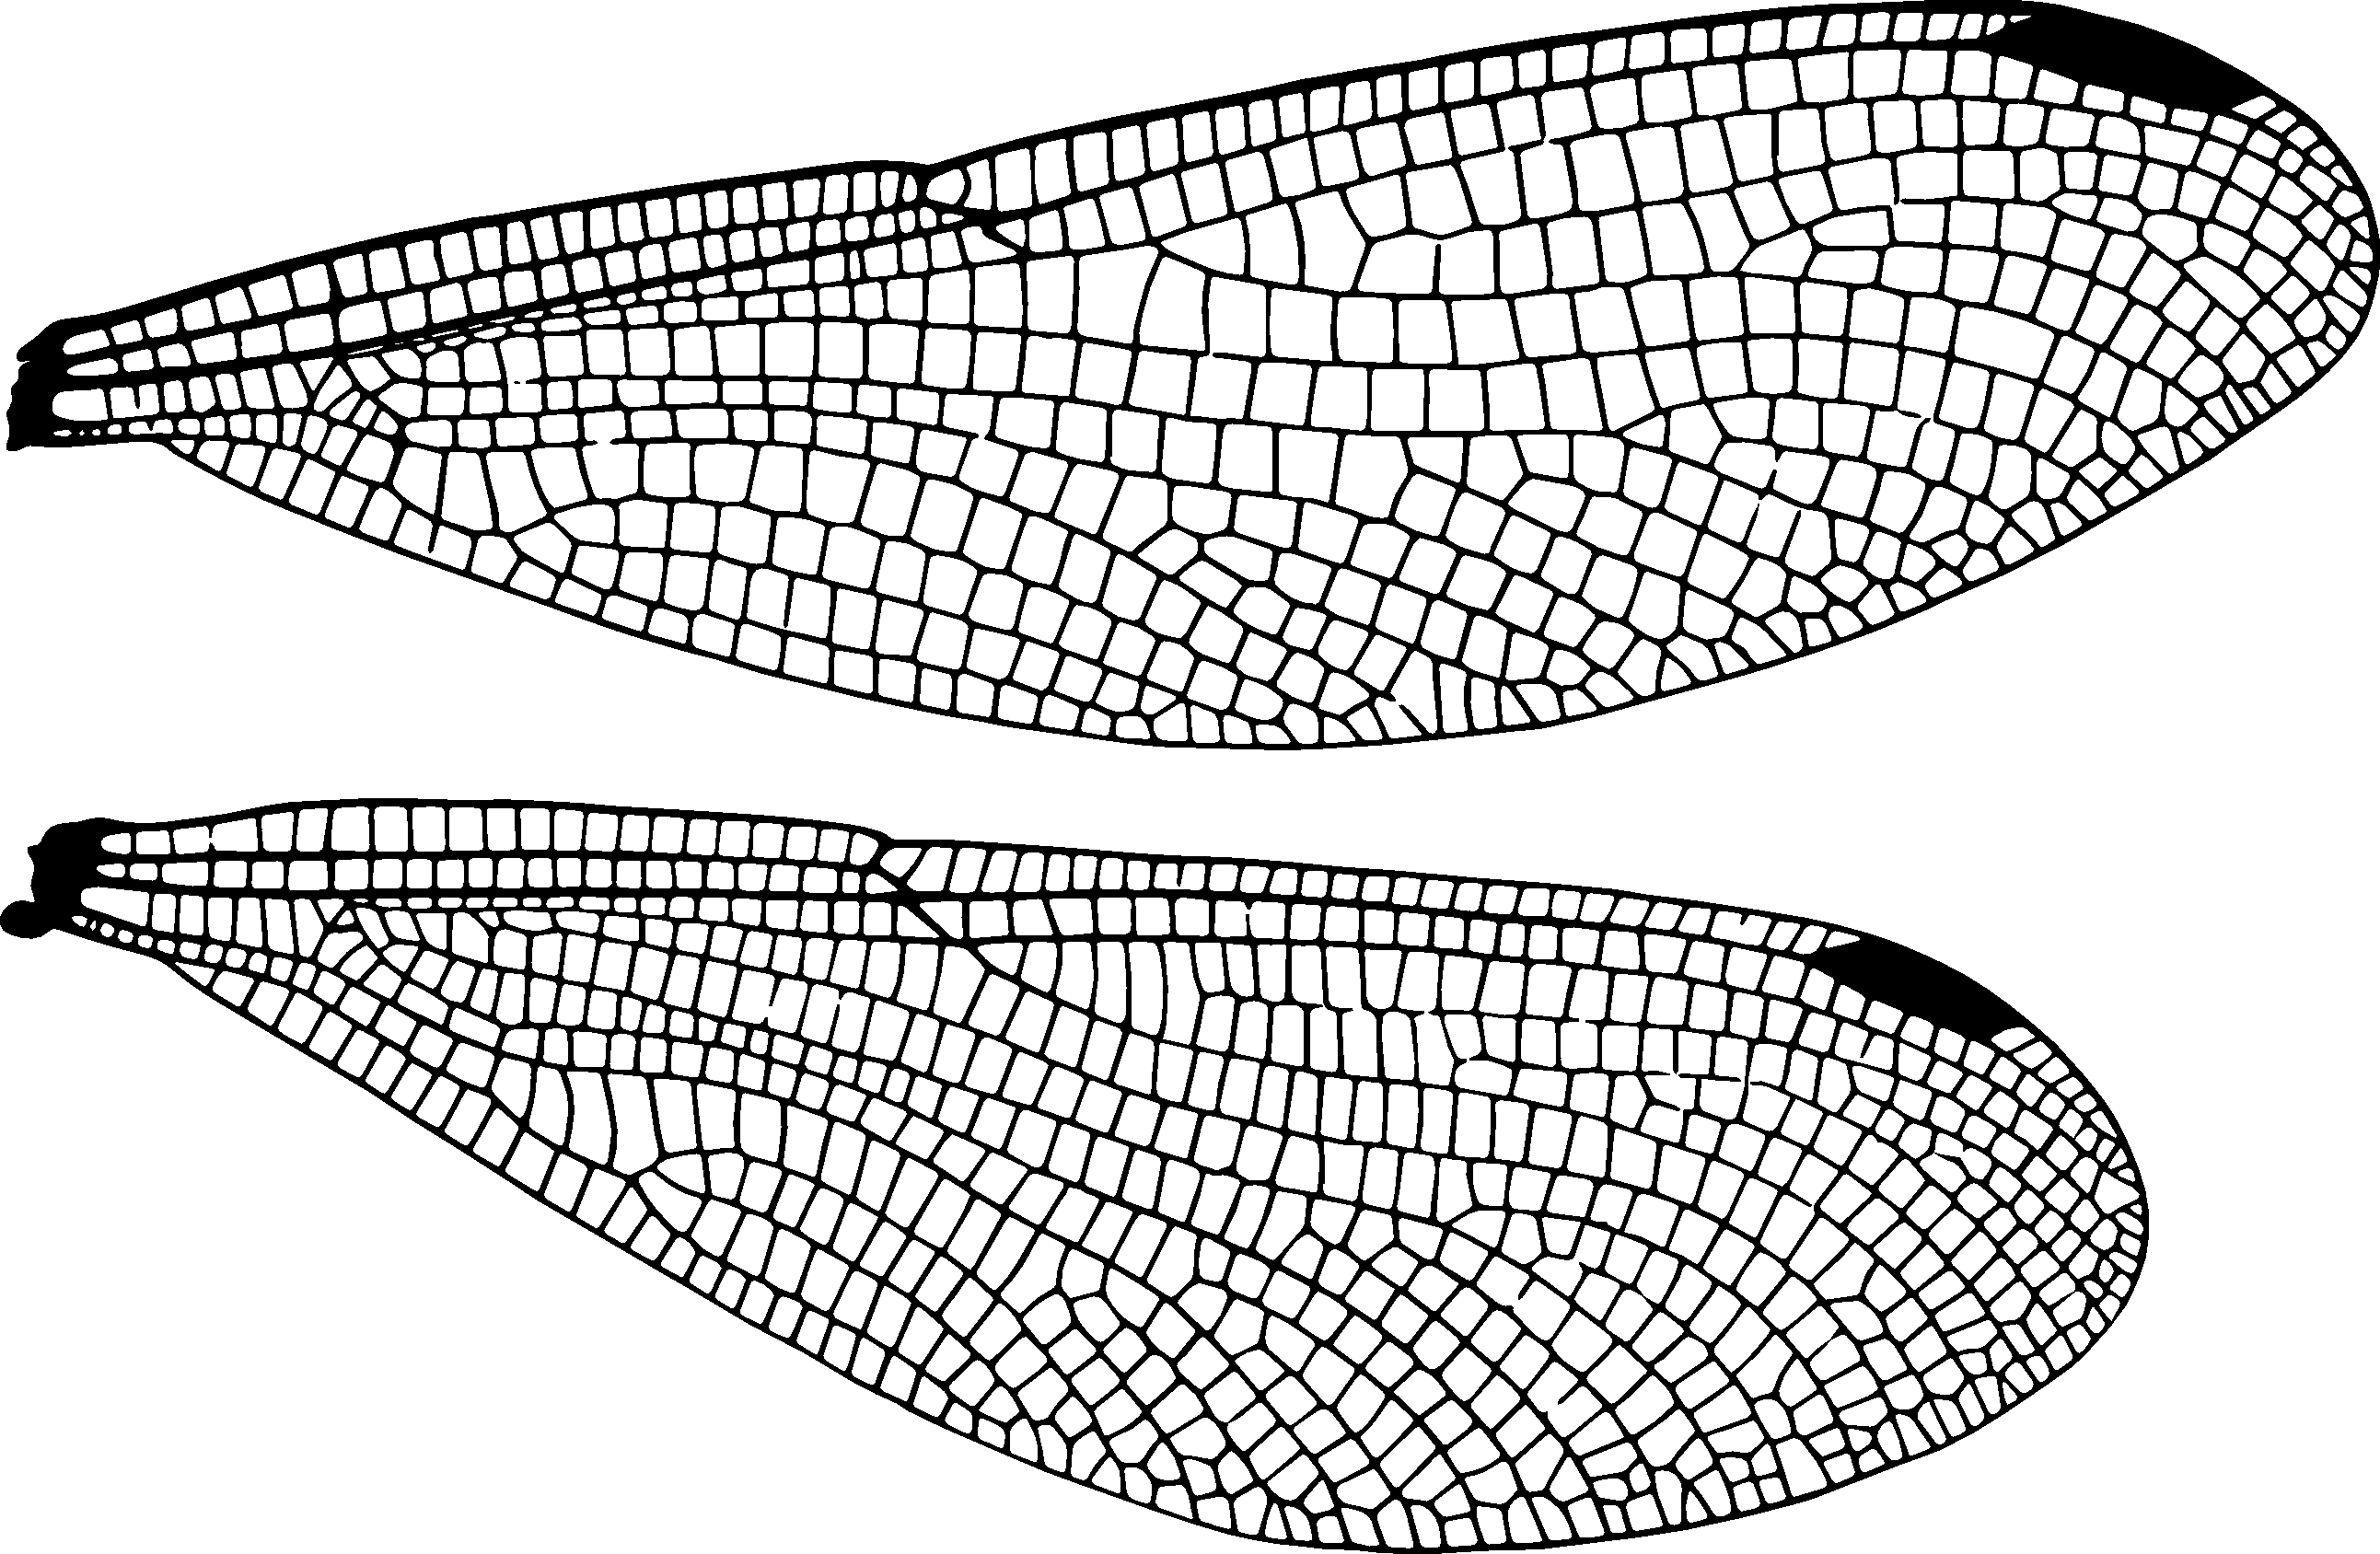
\includegraphics[width=\textwidth]{paleoptera/CalopterygidWing}
        \caption{}
        \label{fig:calopwing}
    \end{subfigure}
    \hfill
    \begin{subfigure}[ht!]{0.45\textwidth}
        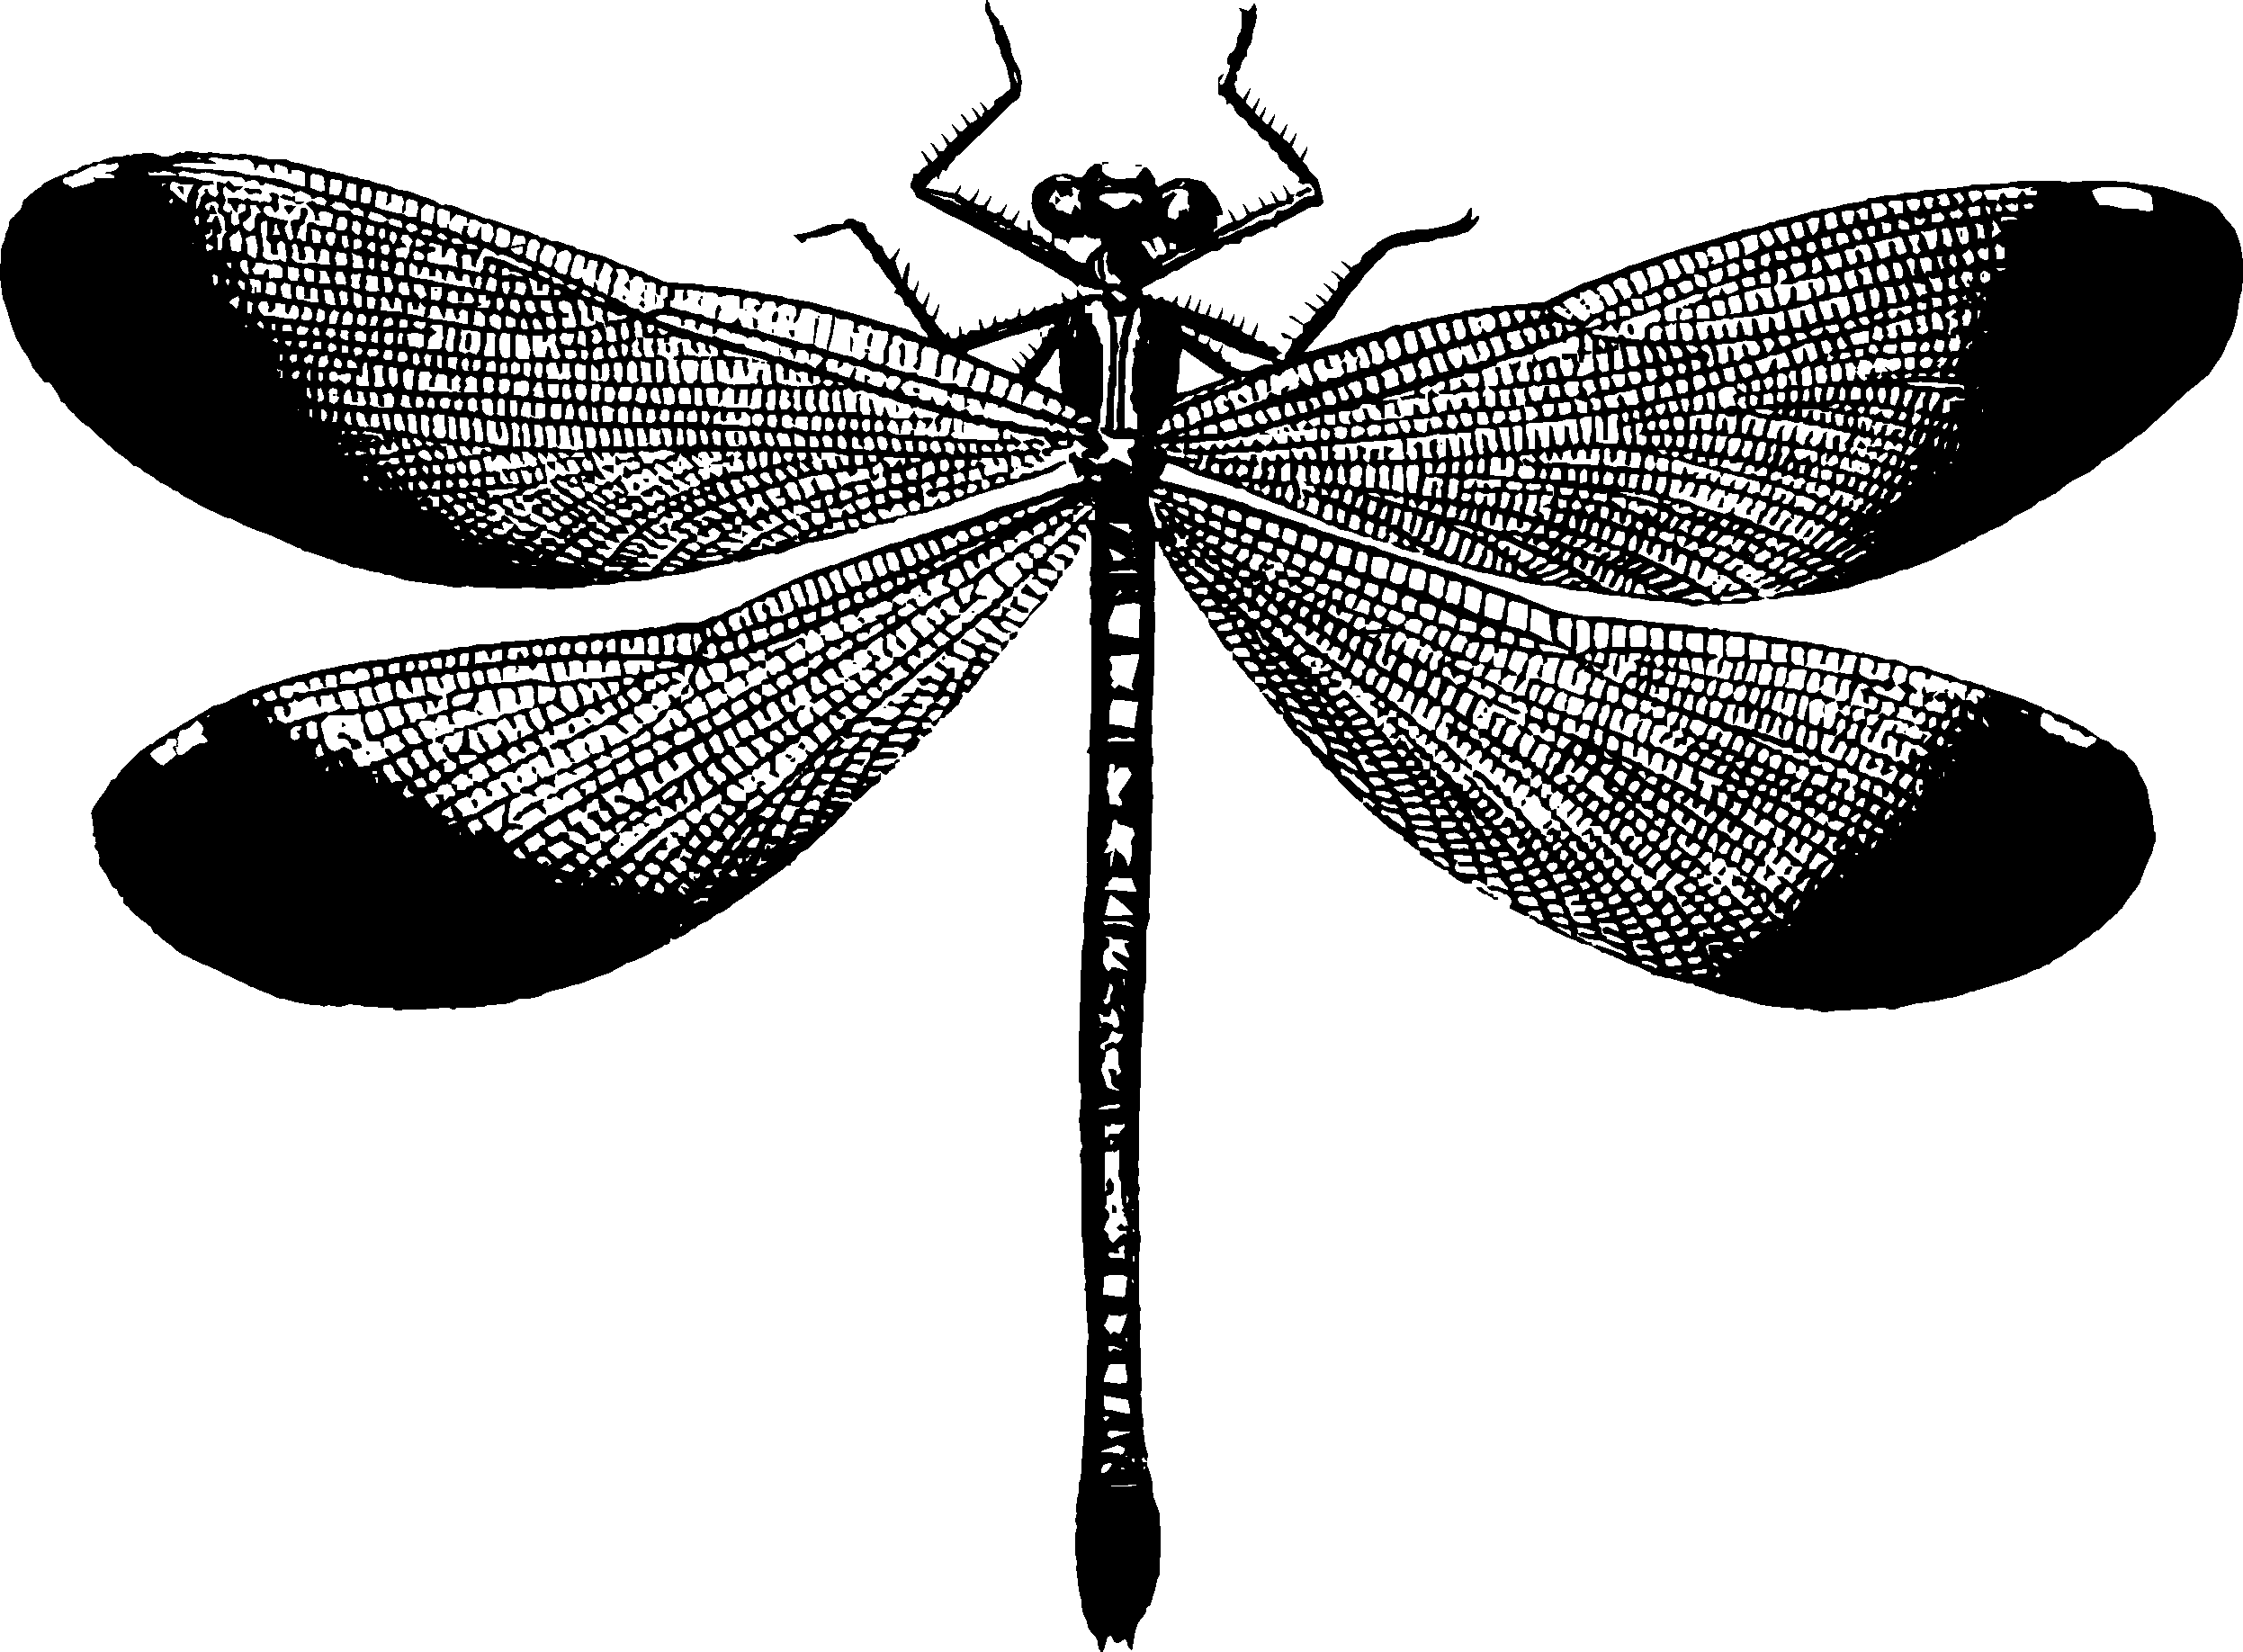
\includegraphics[width=\textwidth]{paleoptera/CalopterygidHabitus}
        \caption{}
        \label{fig:calopbody}
    \end{subfigure}
    \caption{Calopterygidae. \textbf{(a)} Wing venation \citep[][Fig. 235]{comstock1918wings}; \textbf{(b)} habitus \citep[redrawn from][Plate XLVIII, Fig. 2]{bhlitem82229}}\label{fig:calop}
\end{figure}

\subsubsection{Coenagrionidae (bluets, narrow-winged damselflies)}\index{Coenagrionidae}
\noindent{}\textit{Diagnostic characters:} wings stalked at base, few antenodal crossveins present, \texorpdfstring{M\textsubscript{3}}{ }{ } arises near nodus, quadrangle wing cell actually triangular.\vspace{3mm}

\noindent{}\textit{Natural history:} Given the high level of diversity (\textgreater1,100 spp.), one can find these odonates in almost any aquatic habitat. Like other damselflies, larvae are usually thought of as climbers. Females oviposit in or near vegetation.\vspace{3mm}

\begin{figure}[ht!]
    \centering
    \begin{subfigure}[ht!]{0.45\textwidth}
        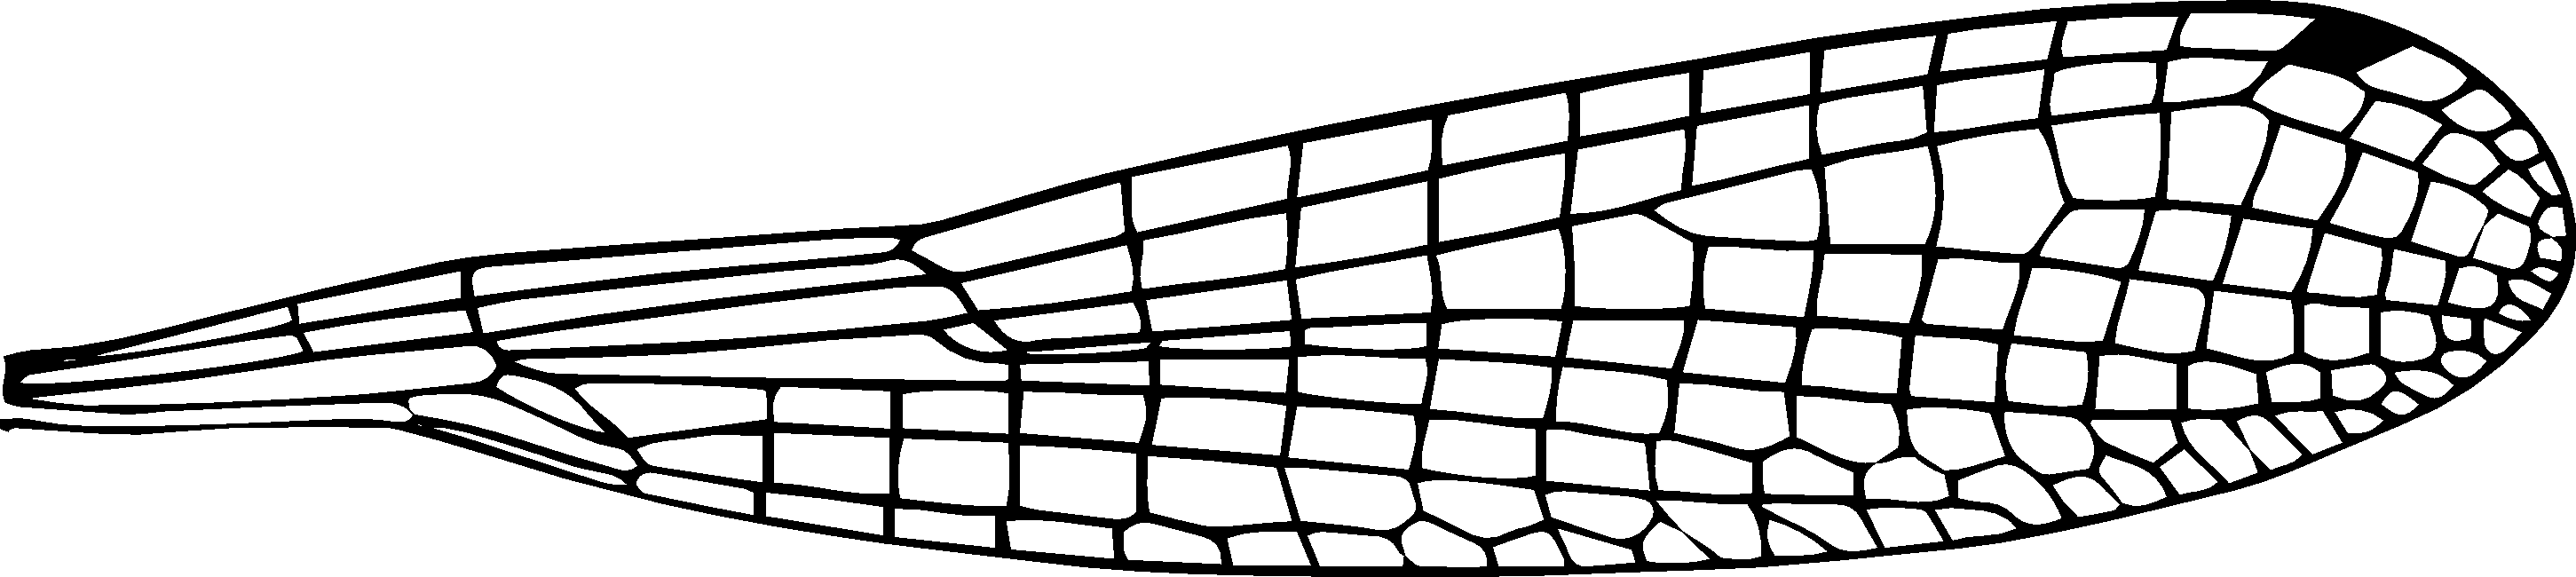
\includegraphics[width=\textwidth]{paleoptera/CoenagrionidWing}
        \caption{}
        \label{fig:coenwing}
    \end{subfigure}
    \hfill
    \begin{subfigure}[ht!]{0.5\textwidth}
        \reflectbox{%
          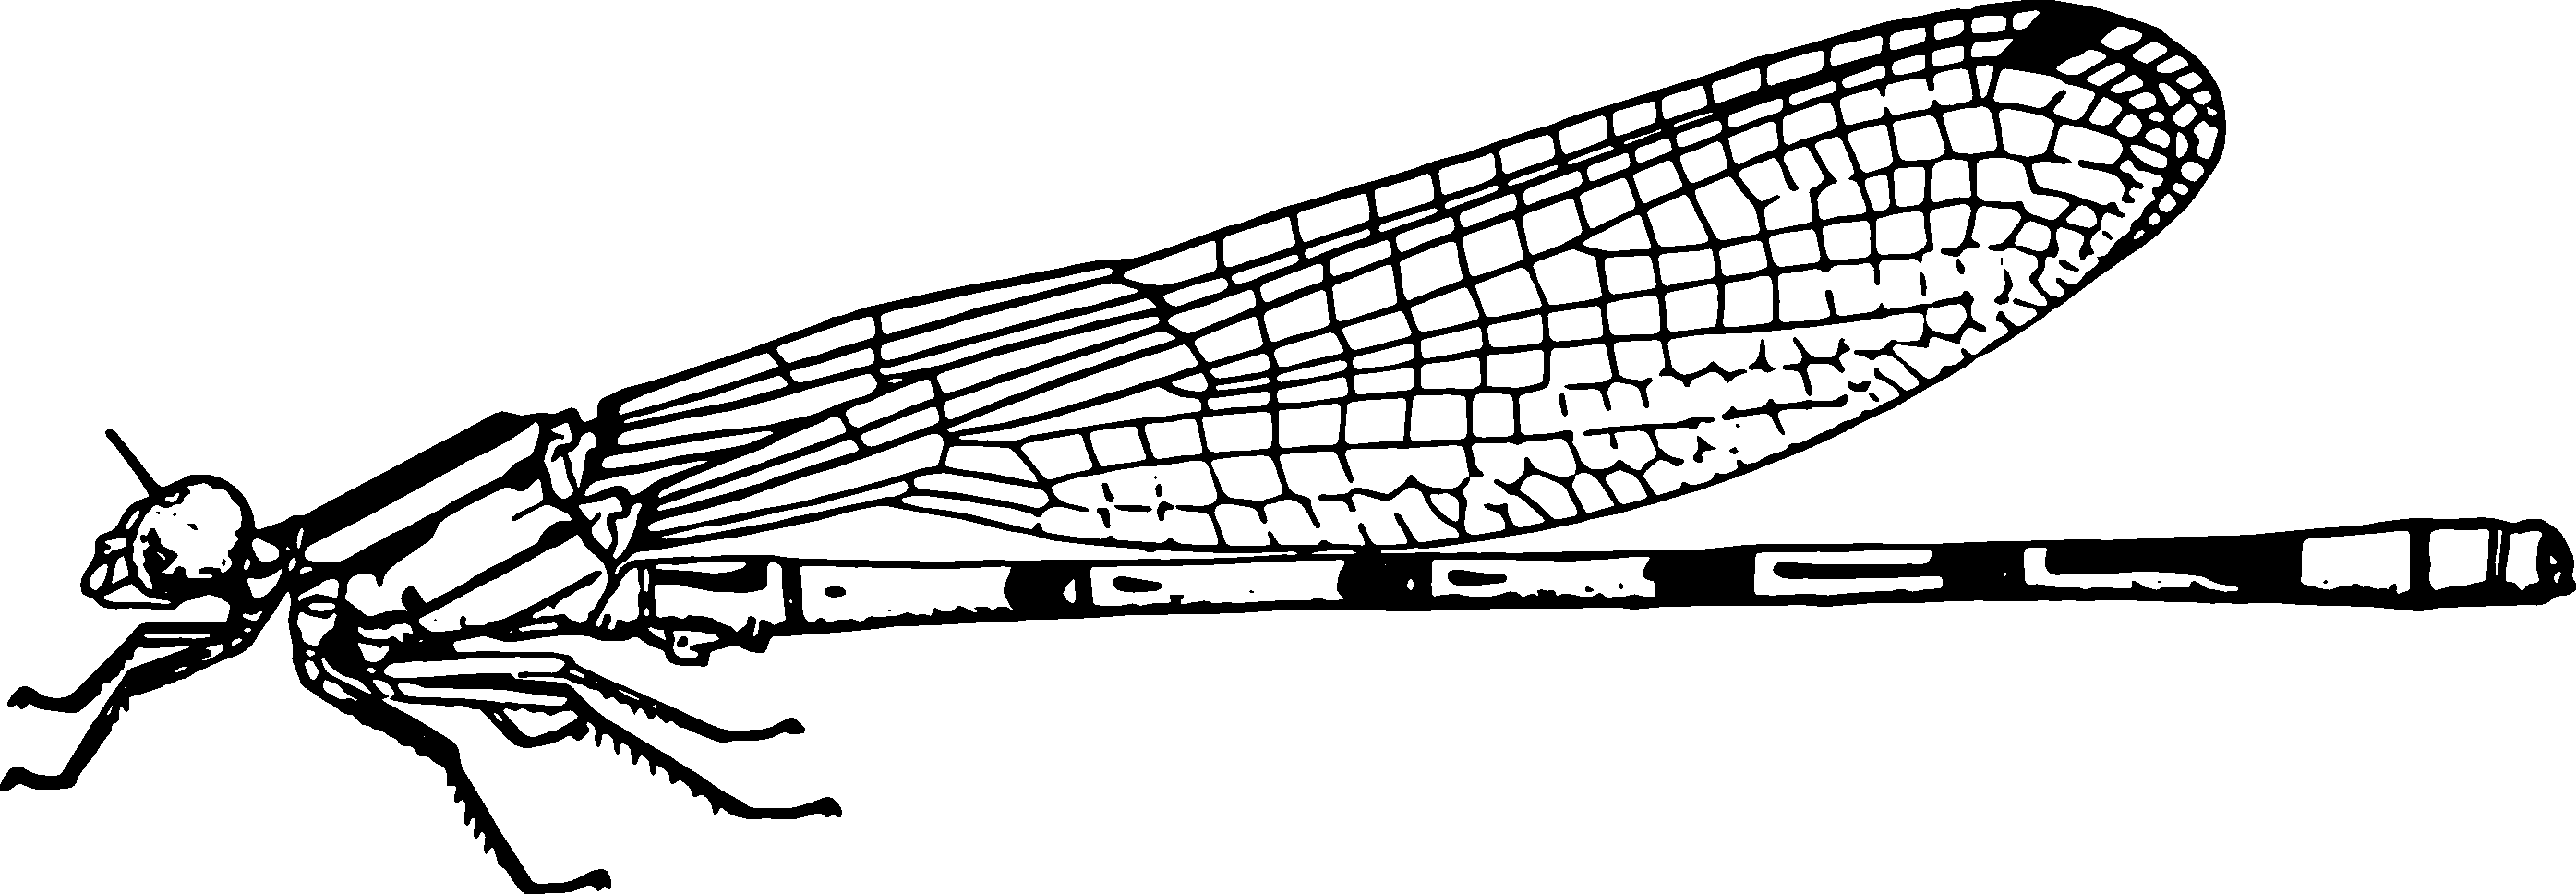
\includegraphics[width=\textwidth]{paleoptera/coenagBody}}
        \caption{}
        \label{fig:coenbody}
    \end{subfigure}
    \caption{Coenagrionidae. \textbf{(a)} Fore wing; \textbf{(b)} habitus \citep[redrawn from][Fig. 4:71a]{bhlitem126080aquatic}}\label{fig:coenag}
\end{figure}

\subsubsection{Lestidae (spreadwings)}\index{Lestidae}
\noindent{}\textit{Diagnostic characters:} wings stalked at base, few antenodal crossveins present, \texorpdfstring{M\textsubscript{3}}{ }{ } arises near arculus, quadrangle wing cell actually quadrangular.\vspace{3mm}

\noindent{}\textit{Natural history:} Naiads are found in a variety of aquatic environments and have a distinctive, elongate habitus and a spoon-like labium. Unlike other damselflies, adult lestids usually rest on vegetation with their wings at least partially spread. Approximately 150 spp. have been described worldwide.\vspace{3mm} 

\begin{figure}[ht!]
    \centering
    \begin{subfigure}[ht!]{0.45\textwidth}
        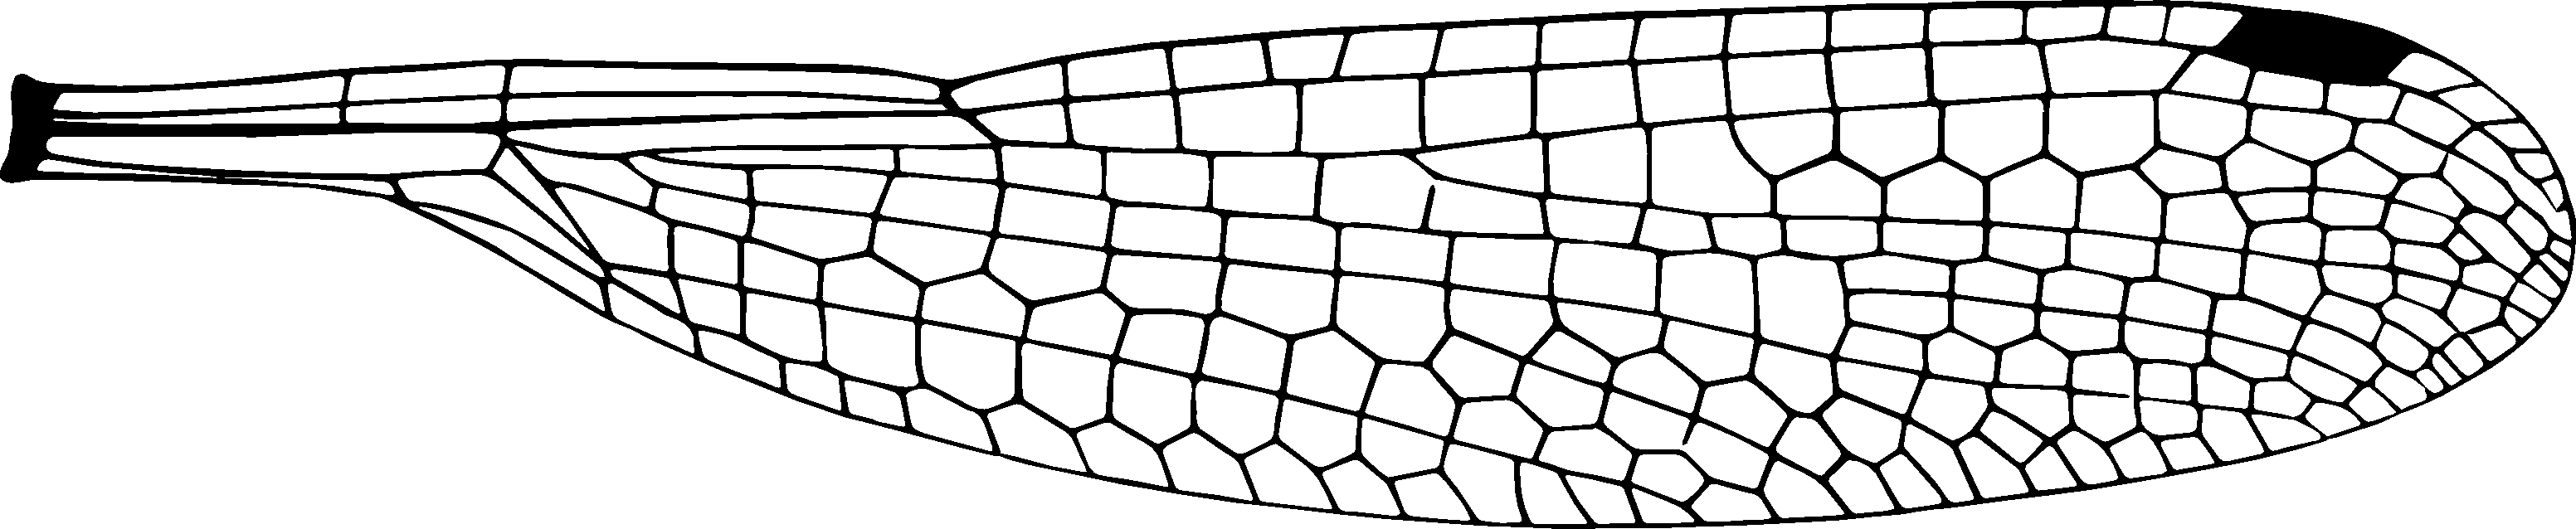
\includegraphics[width=\textwidth]{paleoptera/LestidWing}
        \caption{}
        \label{fig:lestwing}
    \end{subfigure}
    \hfill
    \begin{subfigure}[ht!]{0.45\textwidth}
        \reflectbox{%
          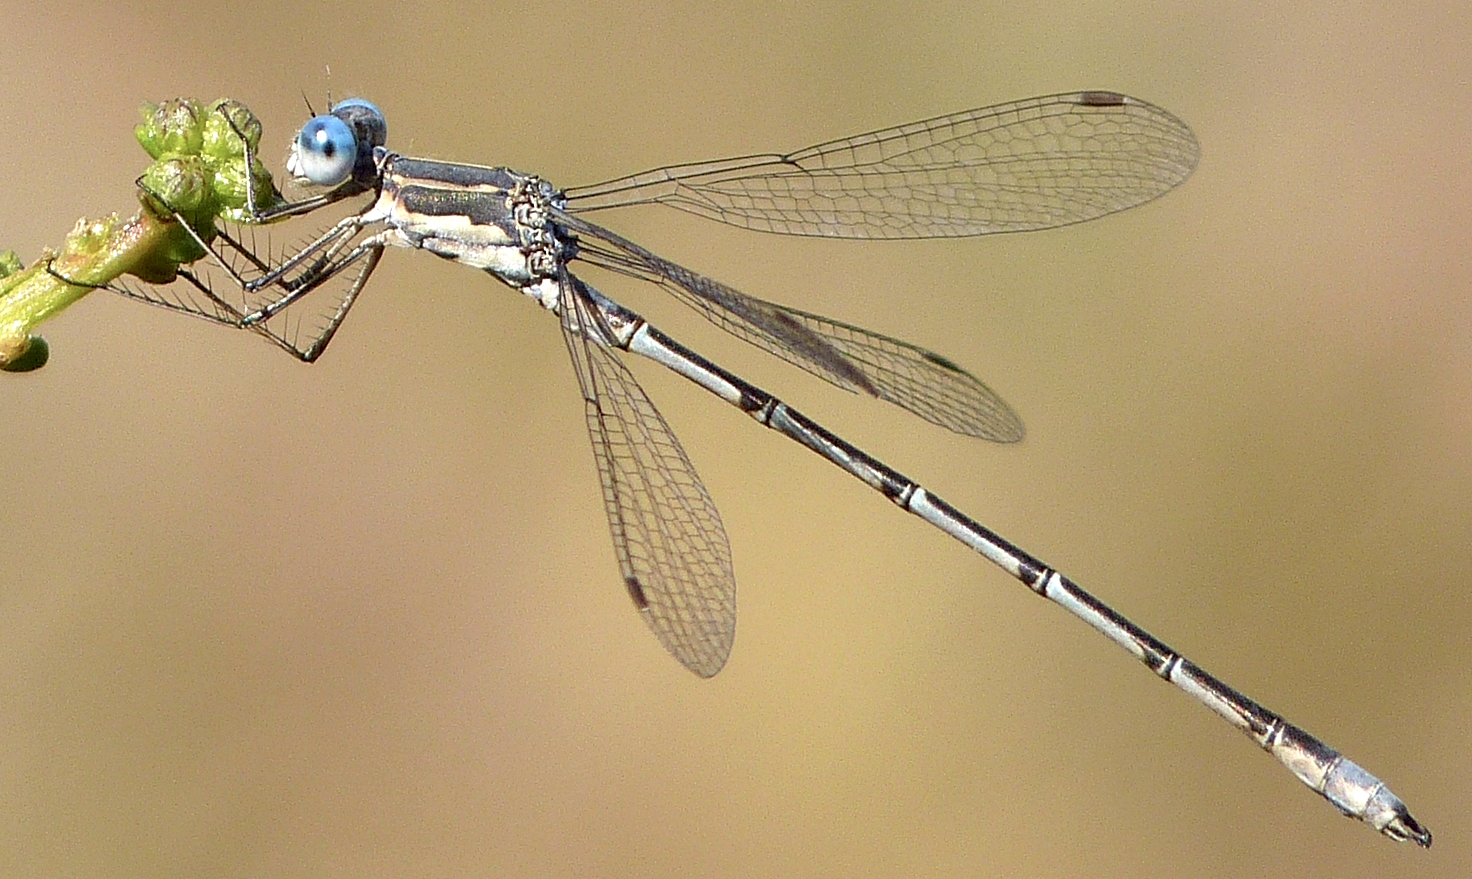
\includegraphics[width=\textwidth]{paleoptera/LestidHabitus}}
        \caption{}
        \label{fig:lestbody}
    \end{subfigure}
    \caption{Lestidae. \textbf{(a)} Wing venation \citep[][Fig. 232]{comstock1918wings}; \textbf{(b)} habitus (illustration by Laura Porturas, Penn State)}\label{fig:lestid}
\end{figure}%https://www.biodiversitylibrary.org/page/40665889

\subsection{Naiads}
Take a moment to observe Odonata naiads of these families under your microscope. Could you determine each family by sight? Can you see the different predatory tactics of the different families?\vspace{3mm}

\begin{theo}
{}Can you find and describe two naiadal adaptations for predation?\vspace{3mm}

\noindent{}What morphological differences to you see between a dragonfly naiad and a damselfly naiad? Make a sketch.
\end{theo}

\begin{figure}[ht!]
    \centering
    \begin{subfigure}[ht!]{0.45\textwidth}
        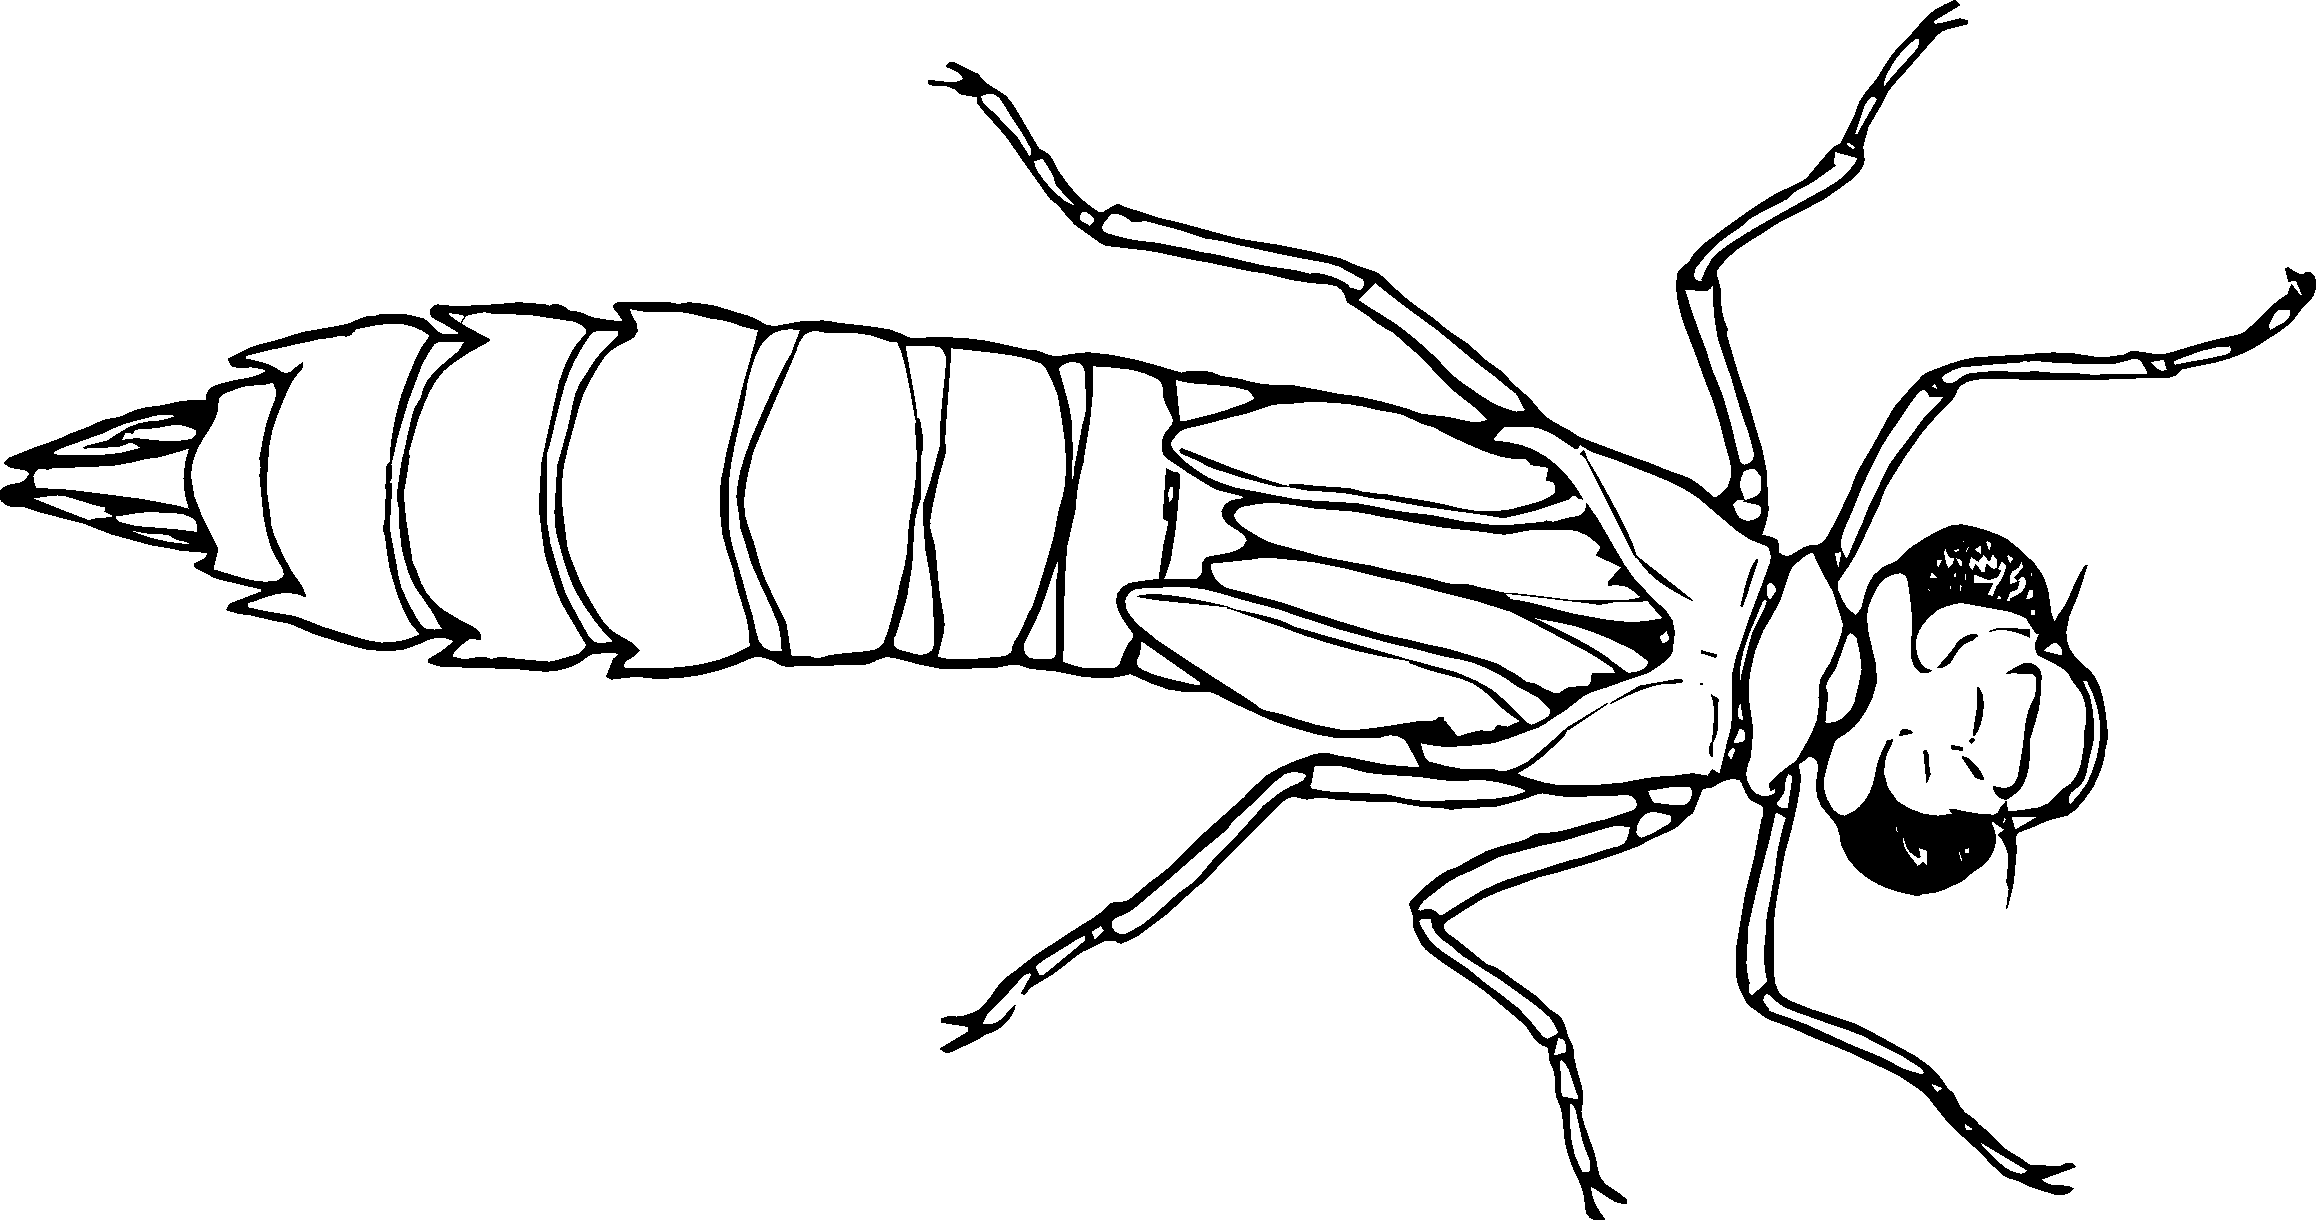
\includegraphics[width=\textwidth]{paleoptera/aeshnidLarva}
        \caption{}
        \label{fig:OdonataLarva}
    \end{subfigure}
    \hfill
    \begin{subfigure}[ht!]{0.47\textwidth}
       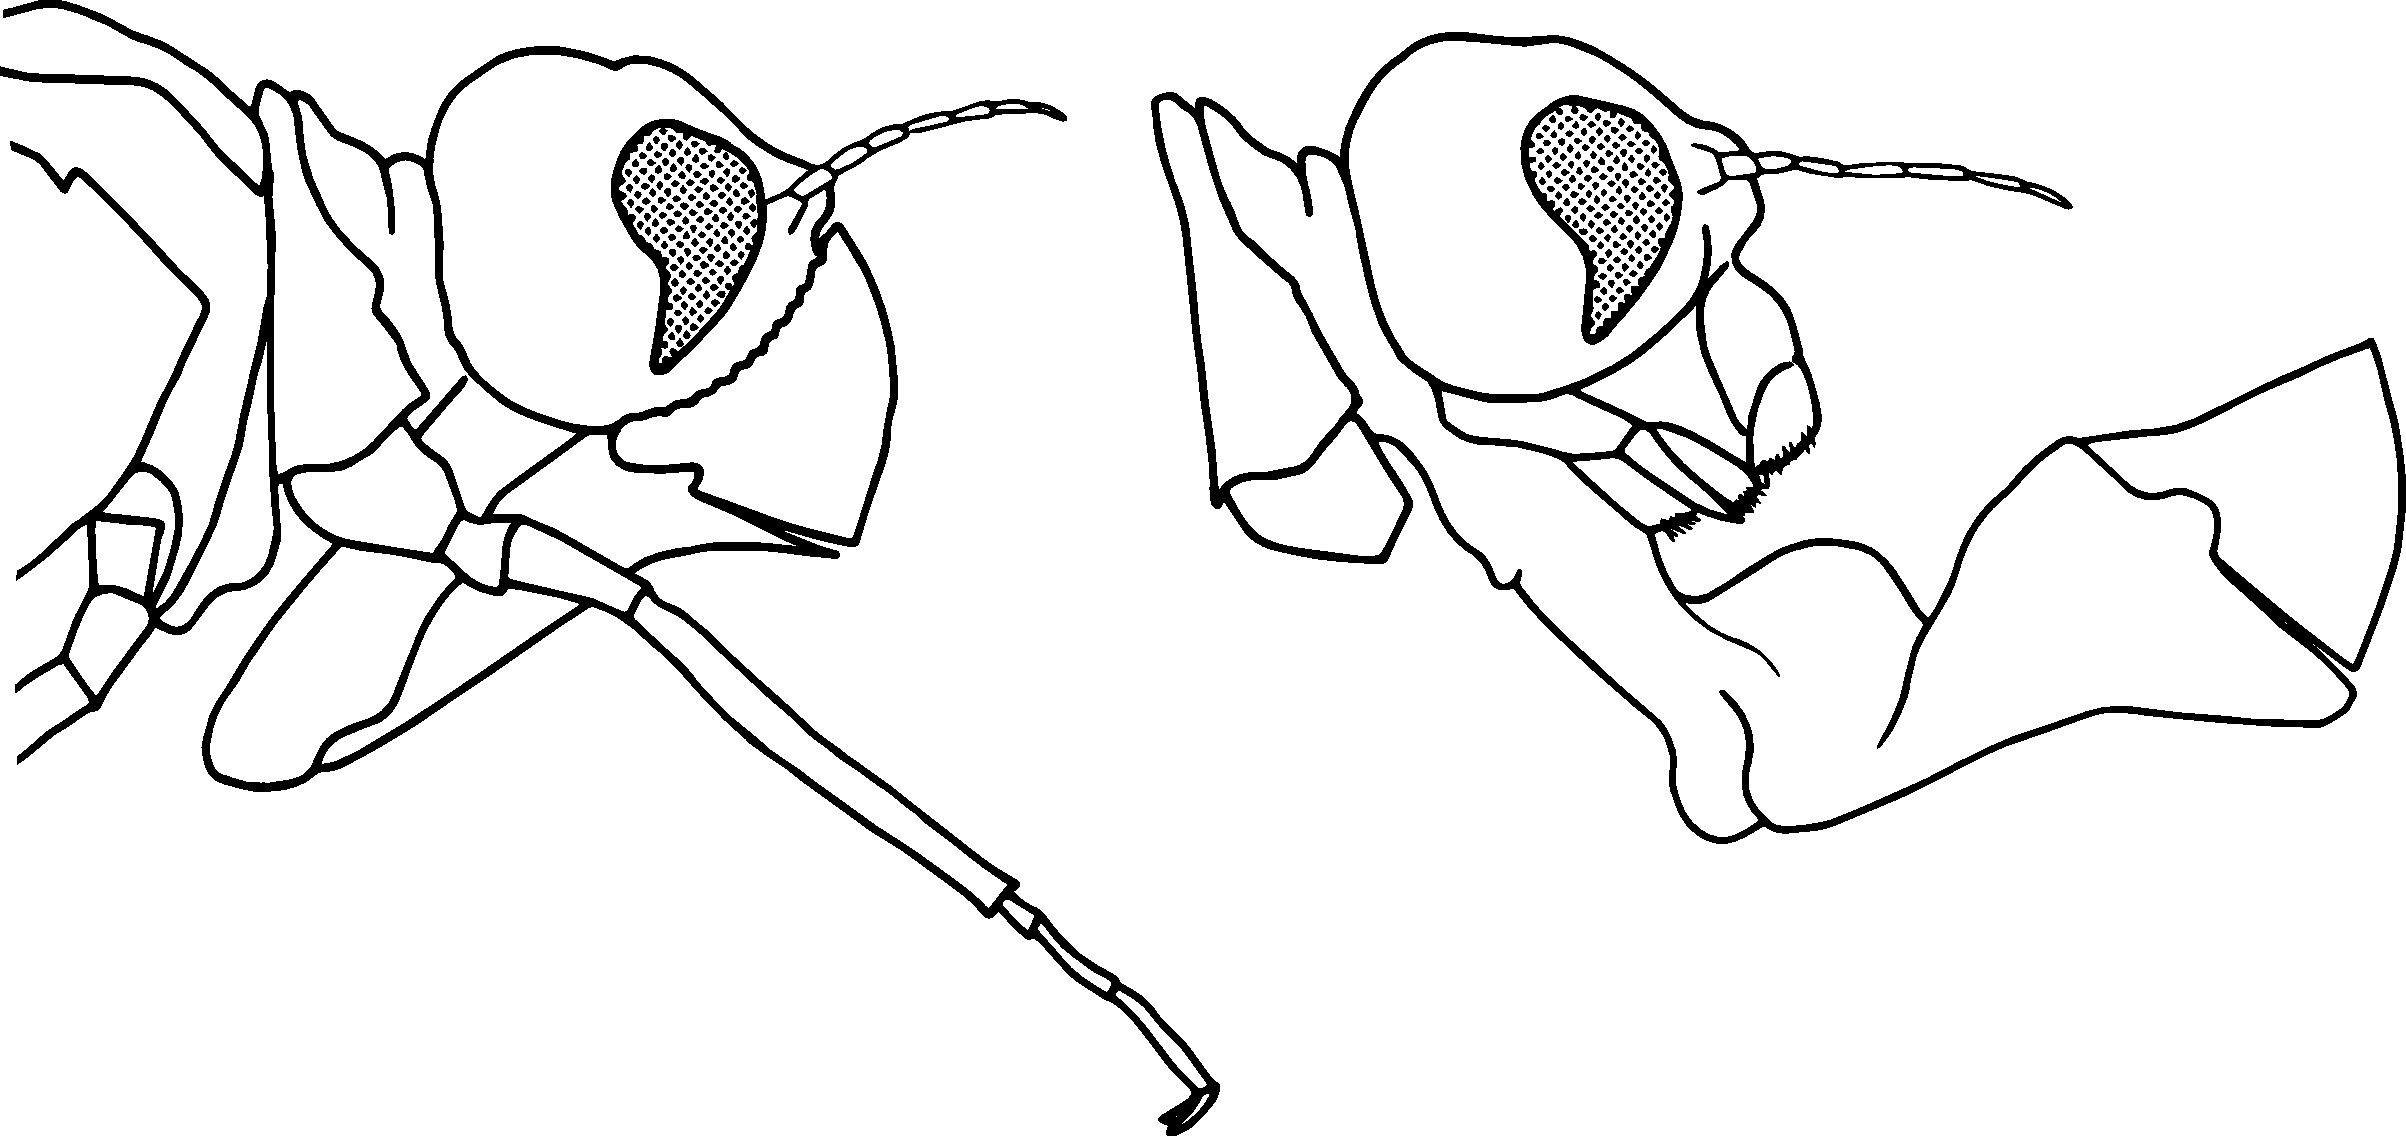
\includegraphics[width=\textwidth]{paleoptera/odonataLarva}
        \caption{}
        \label{fig:OdonataLarvaLabium}
    \end{subfigure}
    \caption{Odonata naiads. \textbf{(a)} Aeshnidae naiad \citep[][Fig. 59]{bhl128276}; \textbf{(b)} libellulid labium, retracted and expanded \citep[redrawn from][Fig. 1]{bhlpart204280odelarva}}\label{fig:odeLarvae}
\end{figure}

\FloatBarrier

\section*{Pterygota: Neoptera}\index{Neoptera}
The remaining insect orders are classified in Neoptera, a lineage whose members can pull their wings over their abdomens when they're at rest. This movement is accomplished by flexing a pleural muscle that inserts on the 3rd axillary sclerite. The wing then folds along flexion lines that are not present in Paleoptera, allowing the wing to be pulled back posteriorly.\vspace{3mm}

\begin{theo}
{}In this unit we've touched on two evolutionary events that are considered to be \latinword{key innovations}: the origin of wings and the the origin of neoptery. Why do you think these two adaptations led to explosive diversification?
\end{theo}

\section{Plecoptera (stoneflies)}\index{Plecoptera}%add Pteronarcyidae (giant stoneflies) and Peltoperlidae (roach-like) need to sight ID?! why not ID the order and describe whether it has gill tufts and nota shape, glossa length, etc.
Like the previous two orders, Plecoptera are aquatic during their immature stages and semi-aquatic/terrestrial as adults. More than 100 million years of evolution separates Plecoptera from Paleoptera \citep{Misof763}, however, so stoneflies are not closely related (relatively speaking) to dragonflies and mayflies. It is useful to treat them here, however, as they have similar habits to mayflies, are important for monitoring water quality (like Ephemeroptera), and have inspired much speculation on the origin of wings.

\subsection*{Naiads}
Stonefly naiads are almost exclusively found in lotic environments---\textit{e.g.}, clear, clean, highly oxygenated streams---and they are generally very sensitive to water quality. The immature stages develop as predators of other aquatic invertebrates or as shredders of vegetative material. They can be recognized from other aquatic non-holometabolous insects by (a) the presence of two tarsal claws on each leg and (b) two cerci on the apex of the abdomen.\vspace{3mm}

\noindent{}Select specimens of at least three families and look for phenotypic differences in these diagnostic traits:
\begin{itemize}
\item presence/absence of gill tufts on the thorax and/or abdomen
\item width and shape of nota in dorsal view
\end{itemize}

\subsection*{Adults}
Stoneflies are generally not good dispersers and so are found near the features from which their naiads emerged. The diagnostic features can be subtle, so it's important to spend some time understanding the relevant morphology:

\begin{itemize}
\item Glossa length relative to paraglossa length (\textit{cf}.\footnote{From the Latin verb \textit{conferre}, to bring together, used here to invite the reader to compare the listed taxa.} Perlidae or Perlodidae \textit{vs}. Leuctridae or Capniidae)
\item Presence/location of gill remnants (\textit{cf}. Perlidae \textit{vs}. Perlodidae. Hint: look near the coxae)
\item Wing phenotype at rest (\textit{cf}. Perlidae or Perlodidae \textit{vs}. Leuctridae)
\item Wing venation (figure \ref{fig:plecowings})
\item Relative length of the cerci (\textit{cf}. Perlidae or Perlodidae \textit{vs}. Leuctridae)
\end{itemize}

\begin{figure}[ht!]
  \centering
    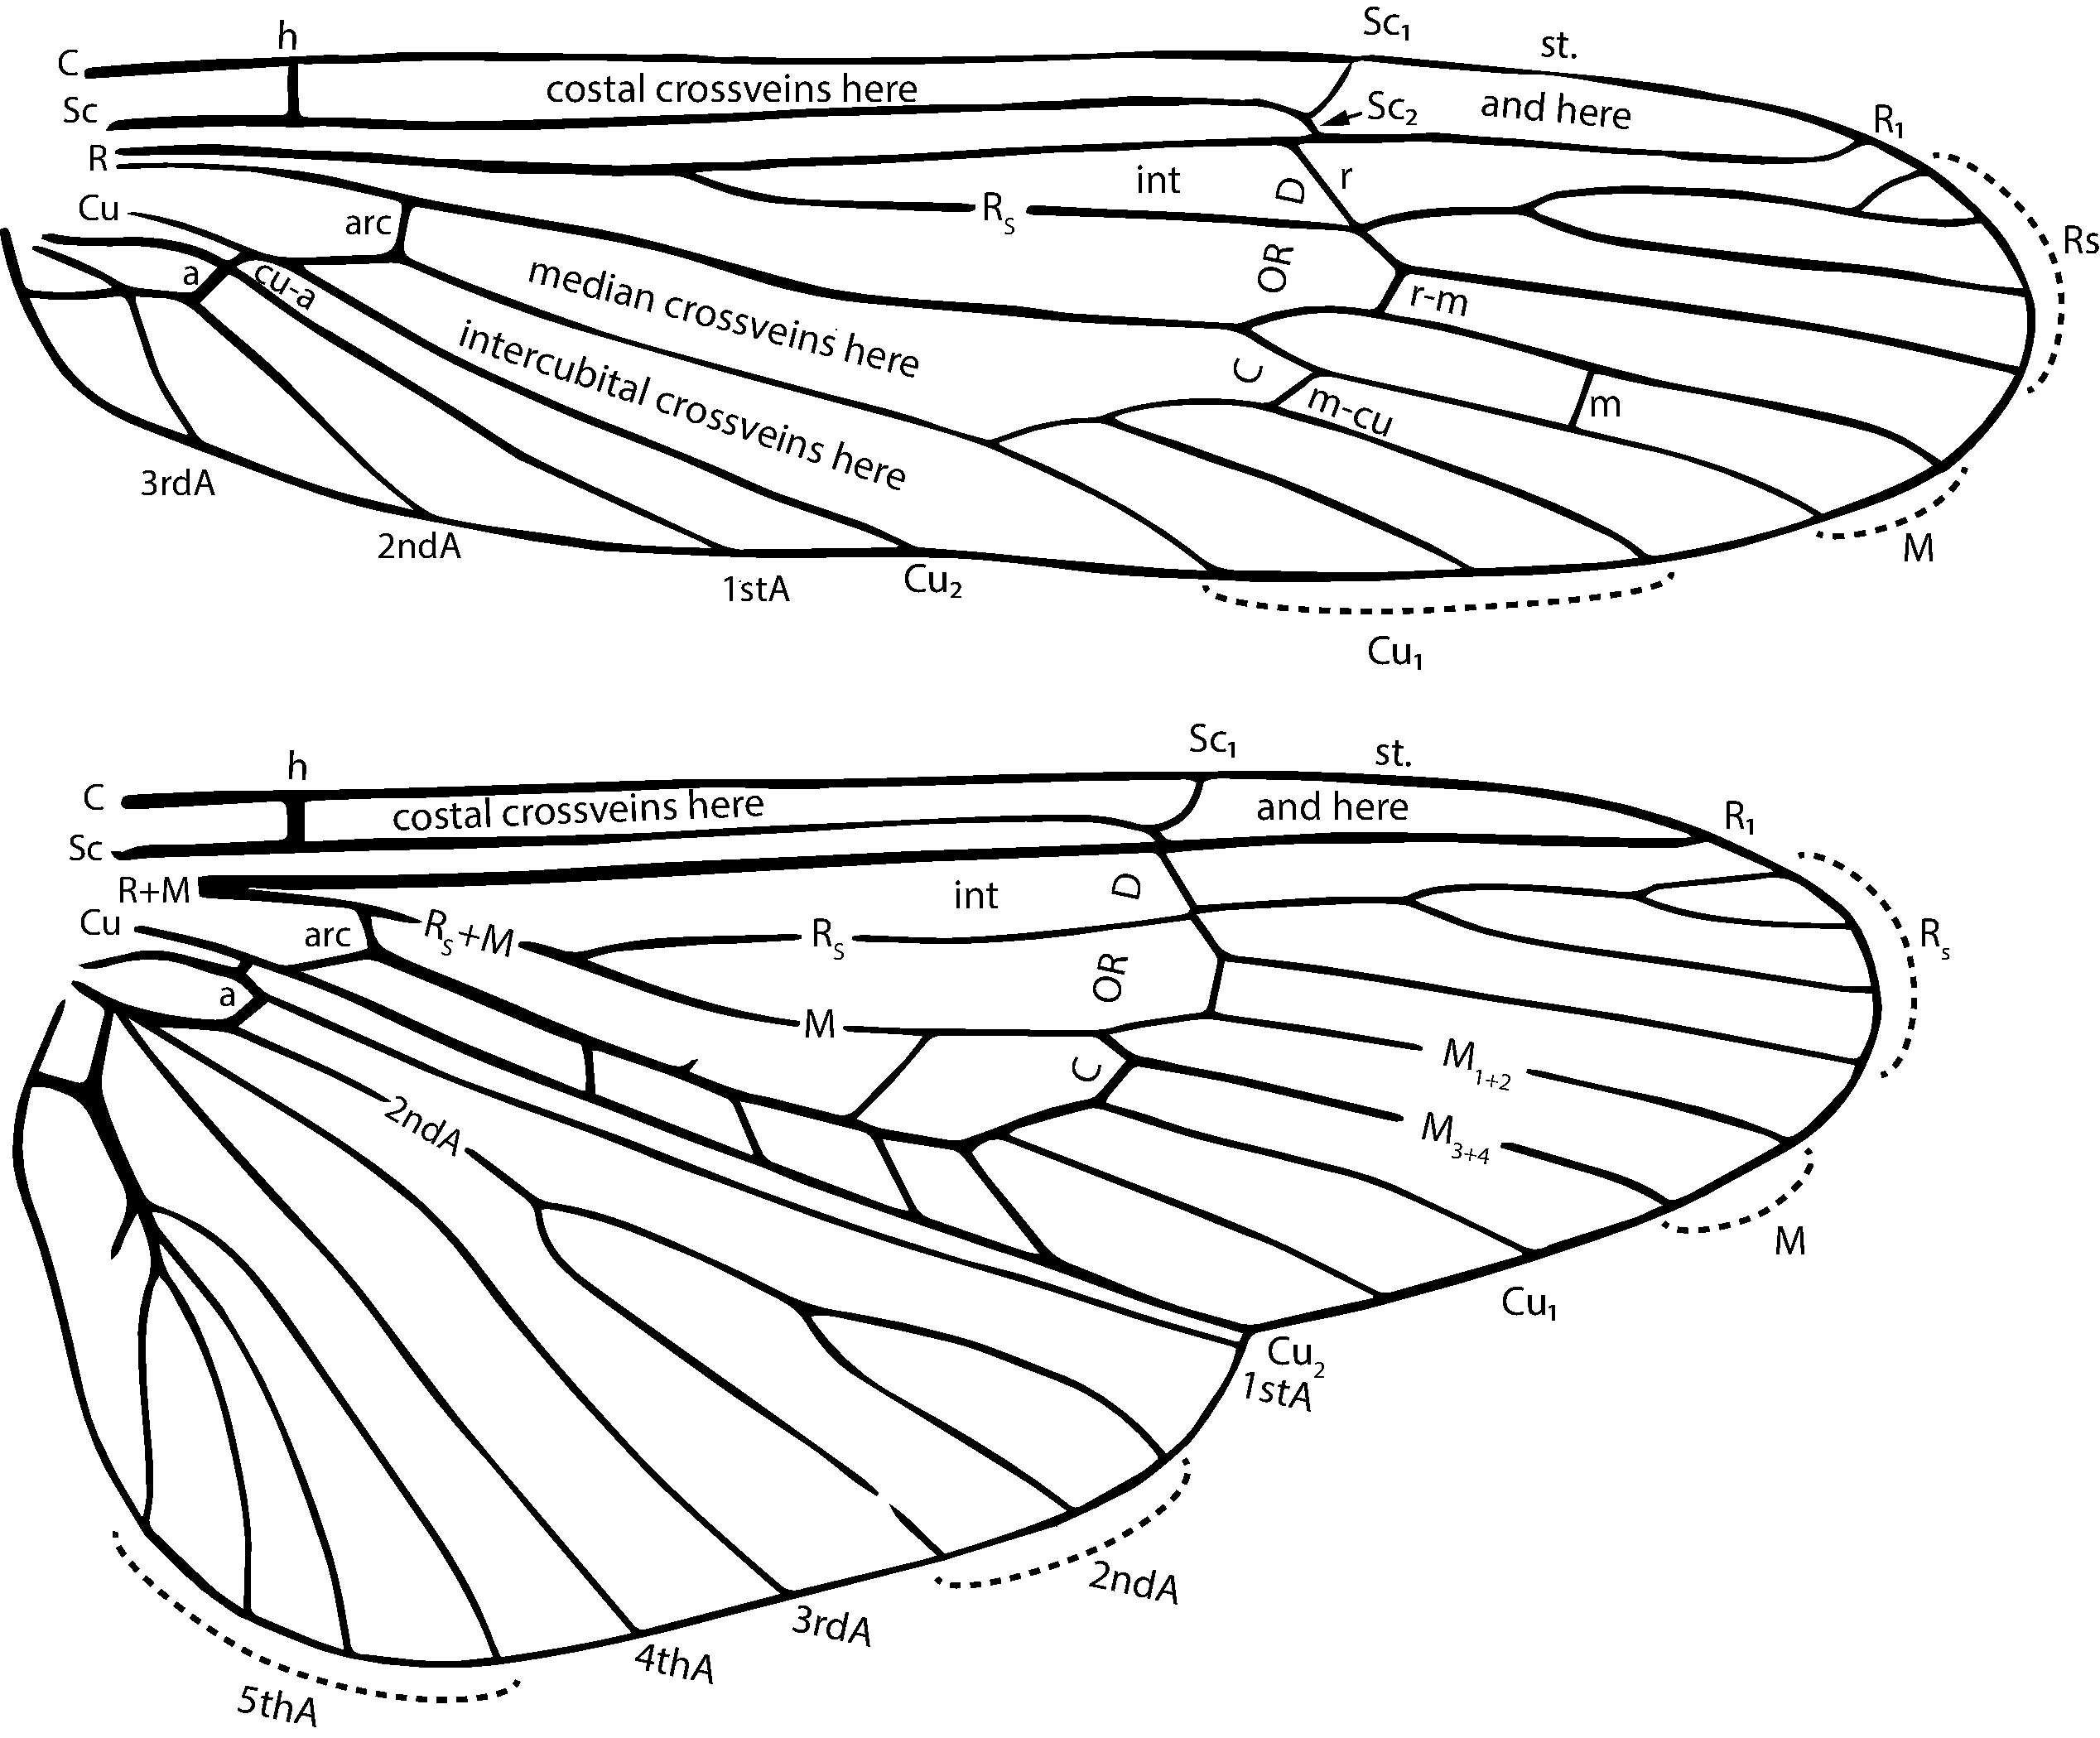
\includegraphics[width=0.65\textwidth]{paleoptera/PlecopteraWings}
  \caption{Plecoptera wing venation \citep[modified from][Fig. 1]{bhl29875}. Caption, from the source and edited slightly: ``C = Costa; Sc = Subcosta; R = Radius; M = Media; Cu = Cubitus; A = Anal; Rs = radial sector, the principal branch of the Radius. A plus sign between letters indicates these veins are fused together. The more typical crossveins are designated as follows: h = humeral; r = inter-radial; r-m = radio-median; m = median; m-cu = medio-cubital crossvein; cu-a = cubito-anal. Other veins and areas are designated as follows: arc = arculus, which is a crossvein to which is often added a deflected basal portion of either of the veins it connects; st = stigma, a thickening in the costal space beyond the tip of the sub-costal vein; a = anal cell; int = inter-radial cell; CORD = the cord, a line of transverse joinings, composed of crossveins and the bases of principal forks, extending from the stigma obliquely backward to the cubital vein. The broad area bounded externally by the cord is sometimes spoken of as the wing disc.''}
  \label{fig:plecowings}
\end{figure}

\subsection{Arctoperlaria}
\subsubsection{Perlidae (common stoneflies)}\index{Perlidae}
\noindent{}\textit{Diagnostic characters:} Glossae much shorter than paraglossae; cercus longer than pronotum width; branched gill remnants present behind leg bases; hind wing with 5 or fewer anal veins; fore wing not rolled around body.\vspace{3mm}

\noindent{}\textit{Natural history:} More than 80 species are known, the vast majority of which can be found in eastern North America. Naiads are predators of other invertebrates.\vspace{3mm} 

\begin{figure}[ht!]
    \centering
    \begin{subfigure}[ht!]{0.45\textwidth}
        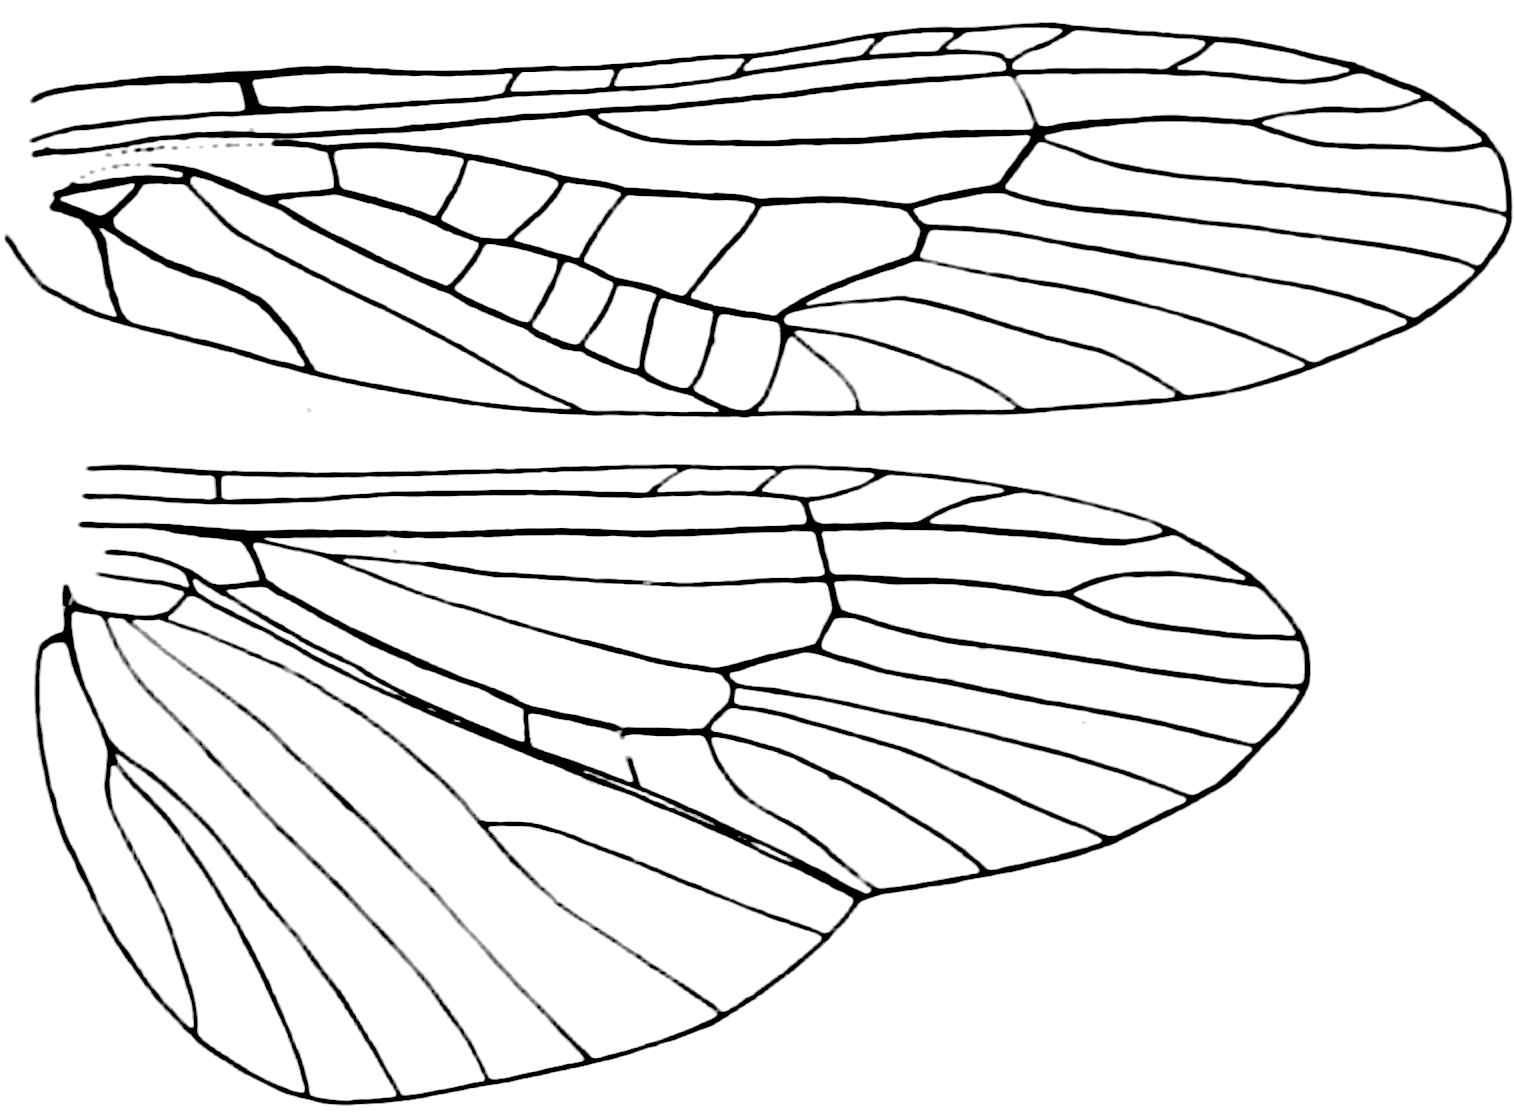
\includegraphics[width=\textwidth]{paleoptera/PerlidWings}
        \caption{}
        \label{fig:perlid1}
    \end{subfigure}
    \qquad
    \begin{subfigure}[ht!]{0.45\textwidth}
        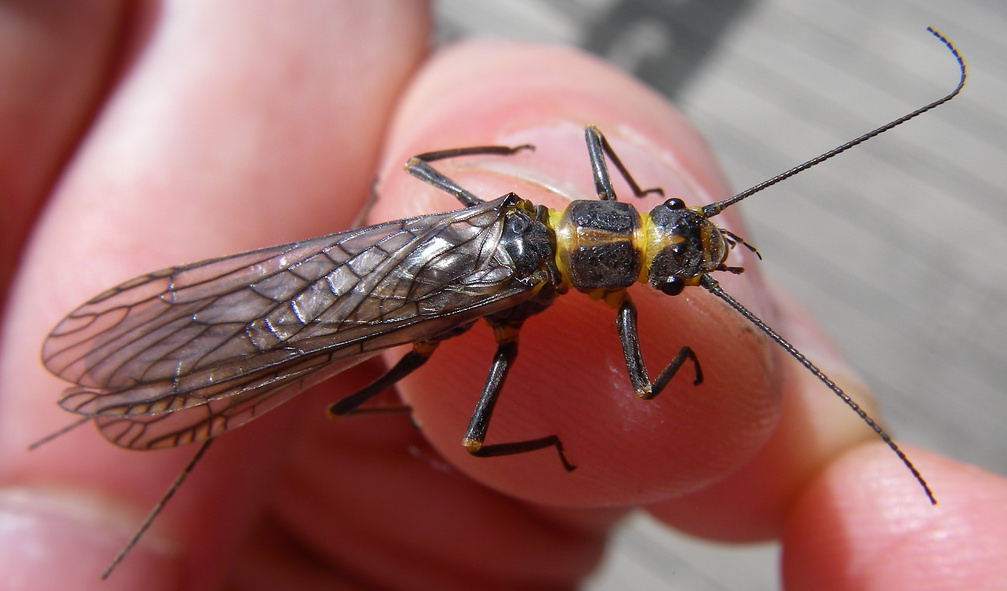
\includegraphics[width=\textwidth]{paleoptera/perlid}
        \caption{}
        \label{fig:perlid2}
    \end{subfigure}
    \caption{Perlidae. \textbf{(a)} Wings \citep[modified from][Plate 11, Fig. 3]{bhl29875}; \textbf{(b)} dorsal habitus \citep[redrawn from][Fig. 18]{bhl29875}}\label{fig:perlids}
\end{figure}

\subsubsection{Perlodidae}\index{Perlodidae}
\noindent{}\textit{Diagnostic characters:} Glossae much shorter than paraglossae; cercus longer than pronotum width; branched gill remnants absent; cubito-anal crossvein arising distal to anal cell; 4 or more Cu crossveins on fore wing, 2A forked; hind wing with 5--10 anal veins; fore wing not rolled around body.\vspace{3mm}

\noindent{}\textit{Natural history:} More than 100 species are known. Naiads are somewhat flattened dorso-ventrally and are predators of other invertebrates.\vspace{3mm}

\begin{figure}[ht!]
    \centering
    \begin{subfigure}[ht!]{0.4\textwidth}
        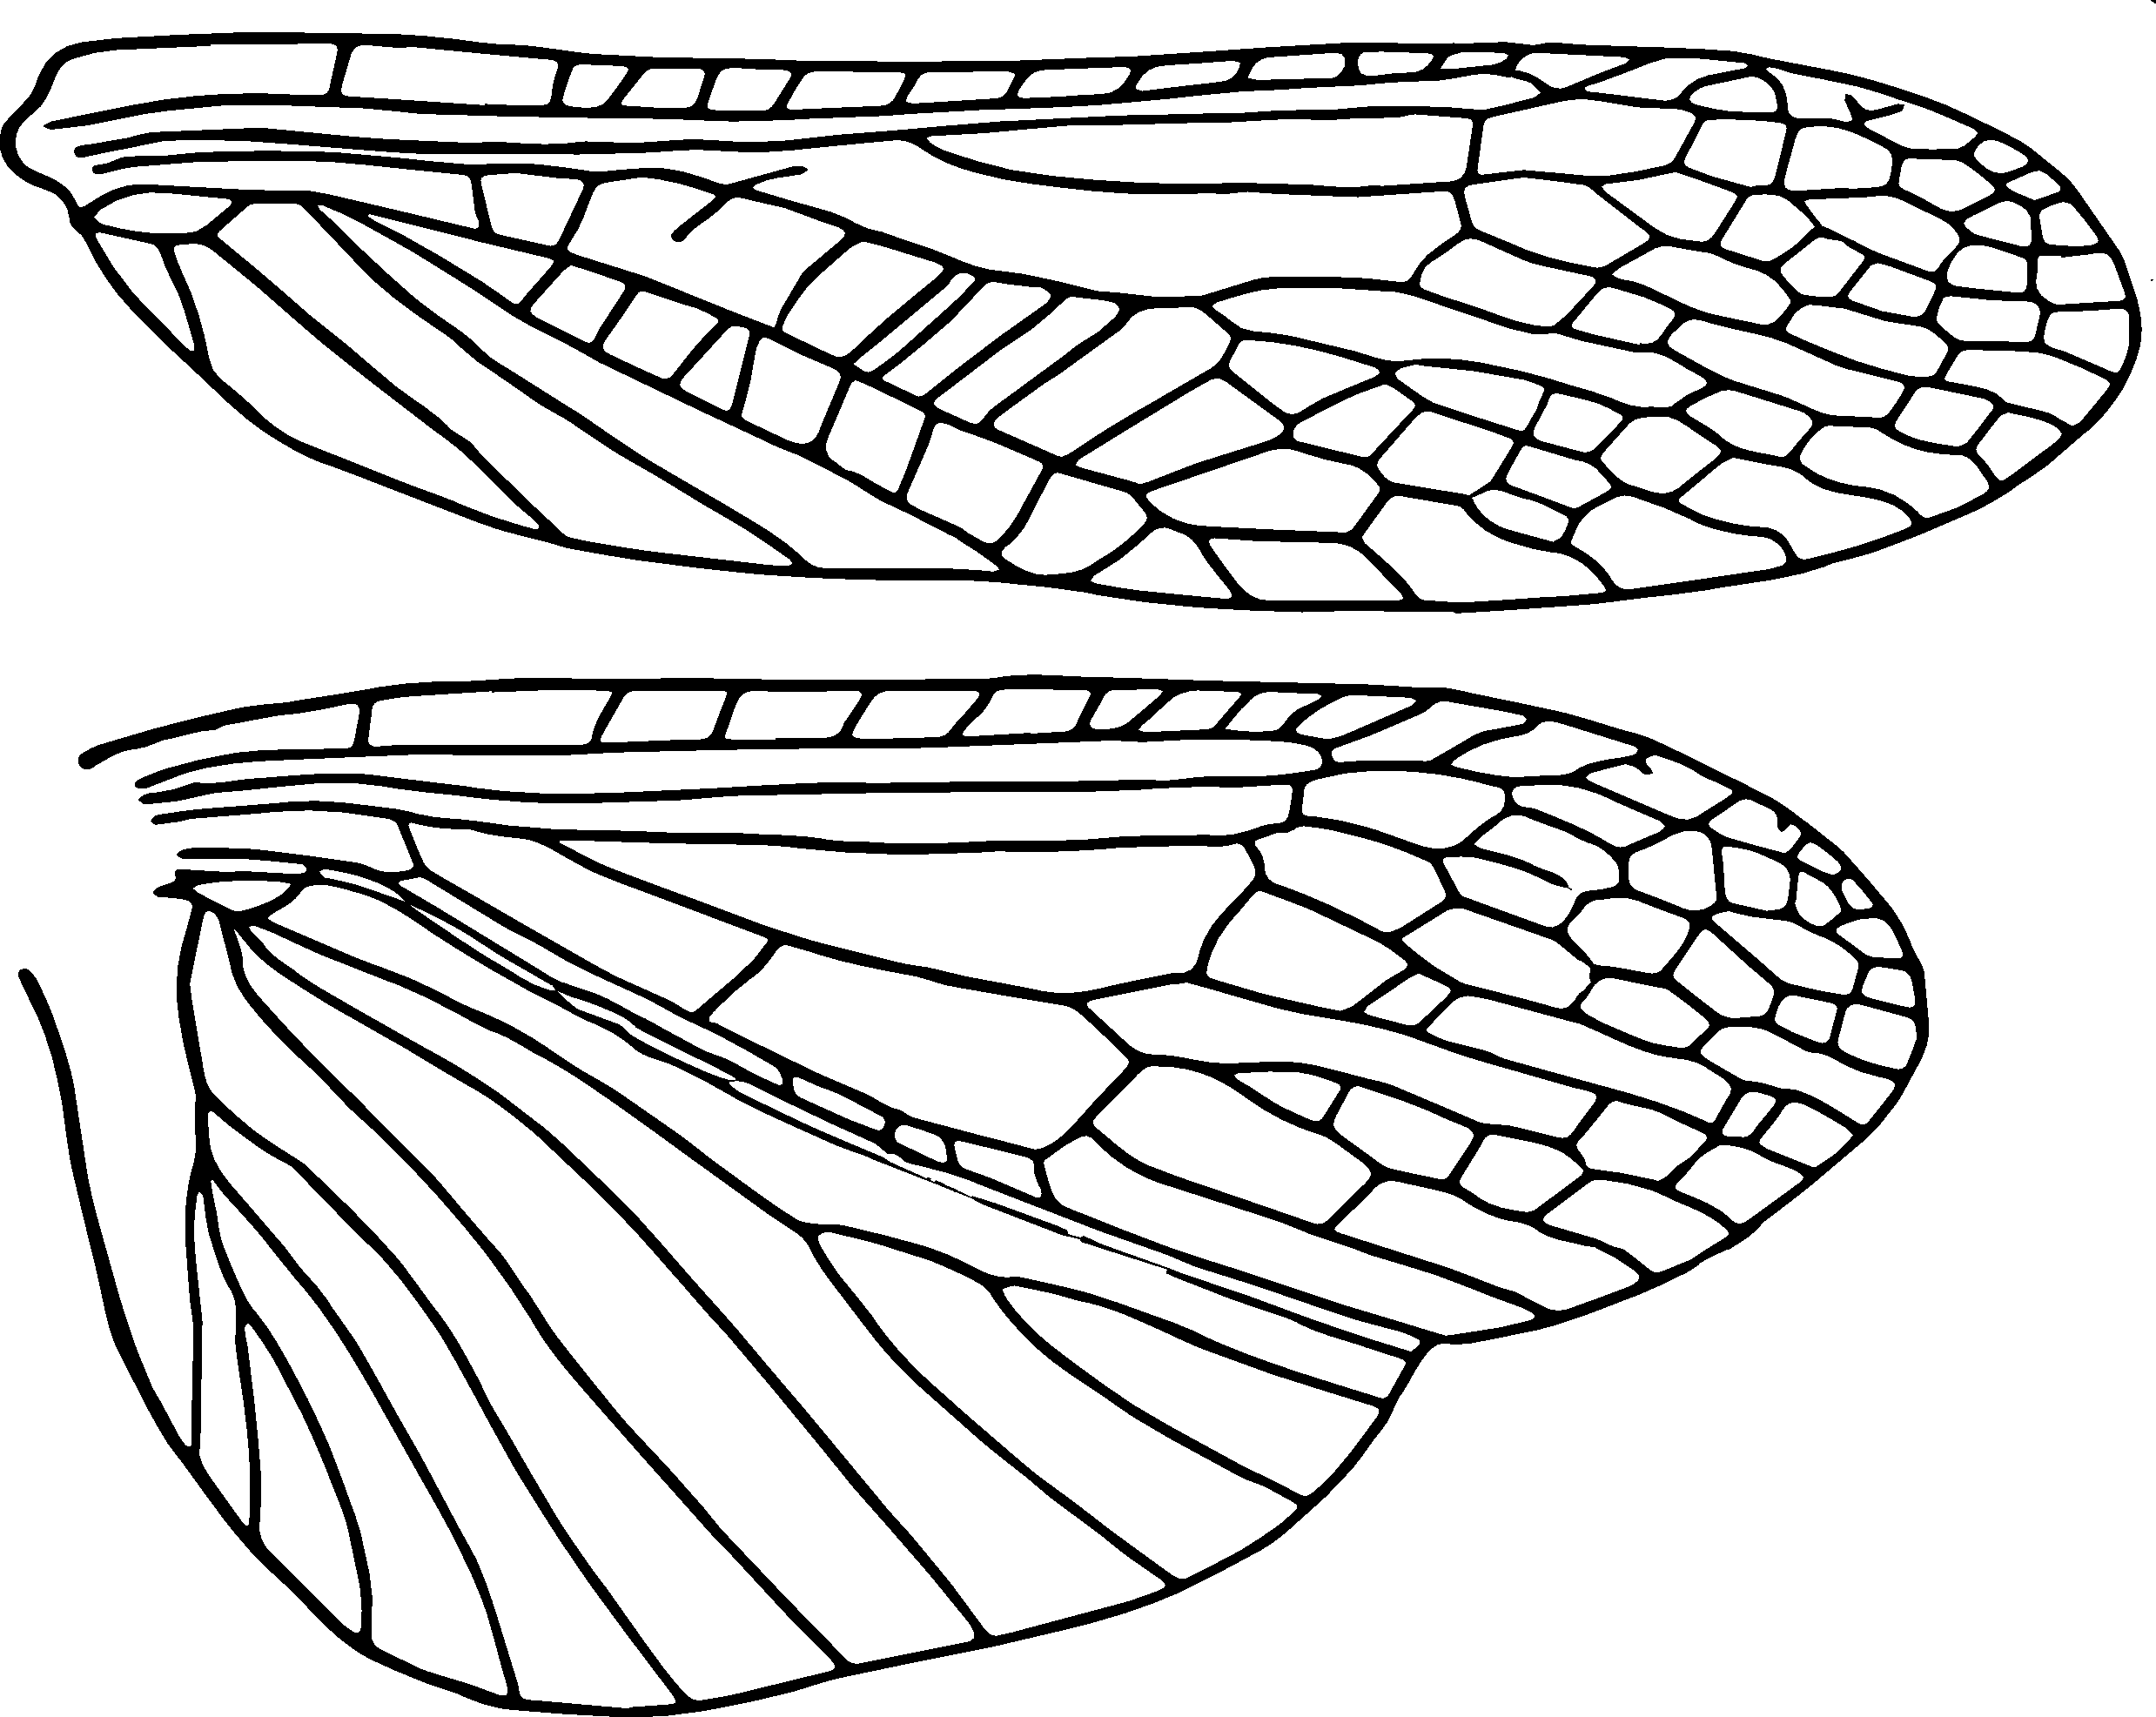
\includegraphics[width=\textwidth]{paleoptera/PerlodidWings}
        \caption{}
        \label{fig:perlodid1}
    \end{subfigure}
    \qquad
    \begin{subfigure}[ht!]{0.5\textwidth}
        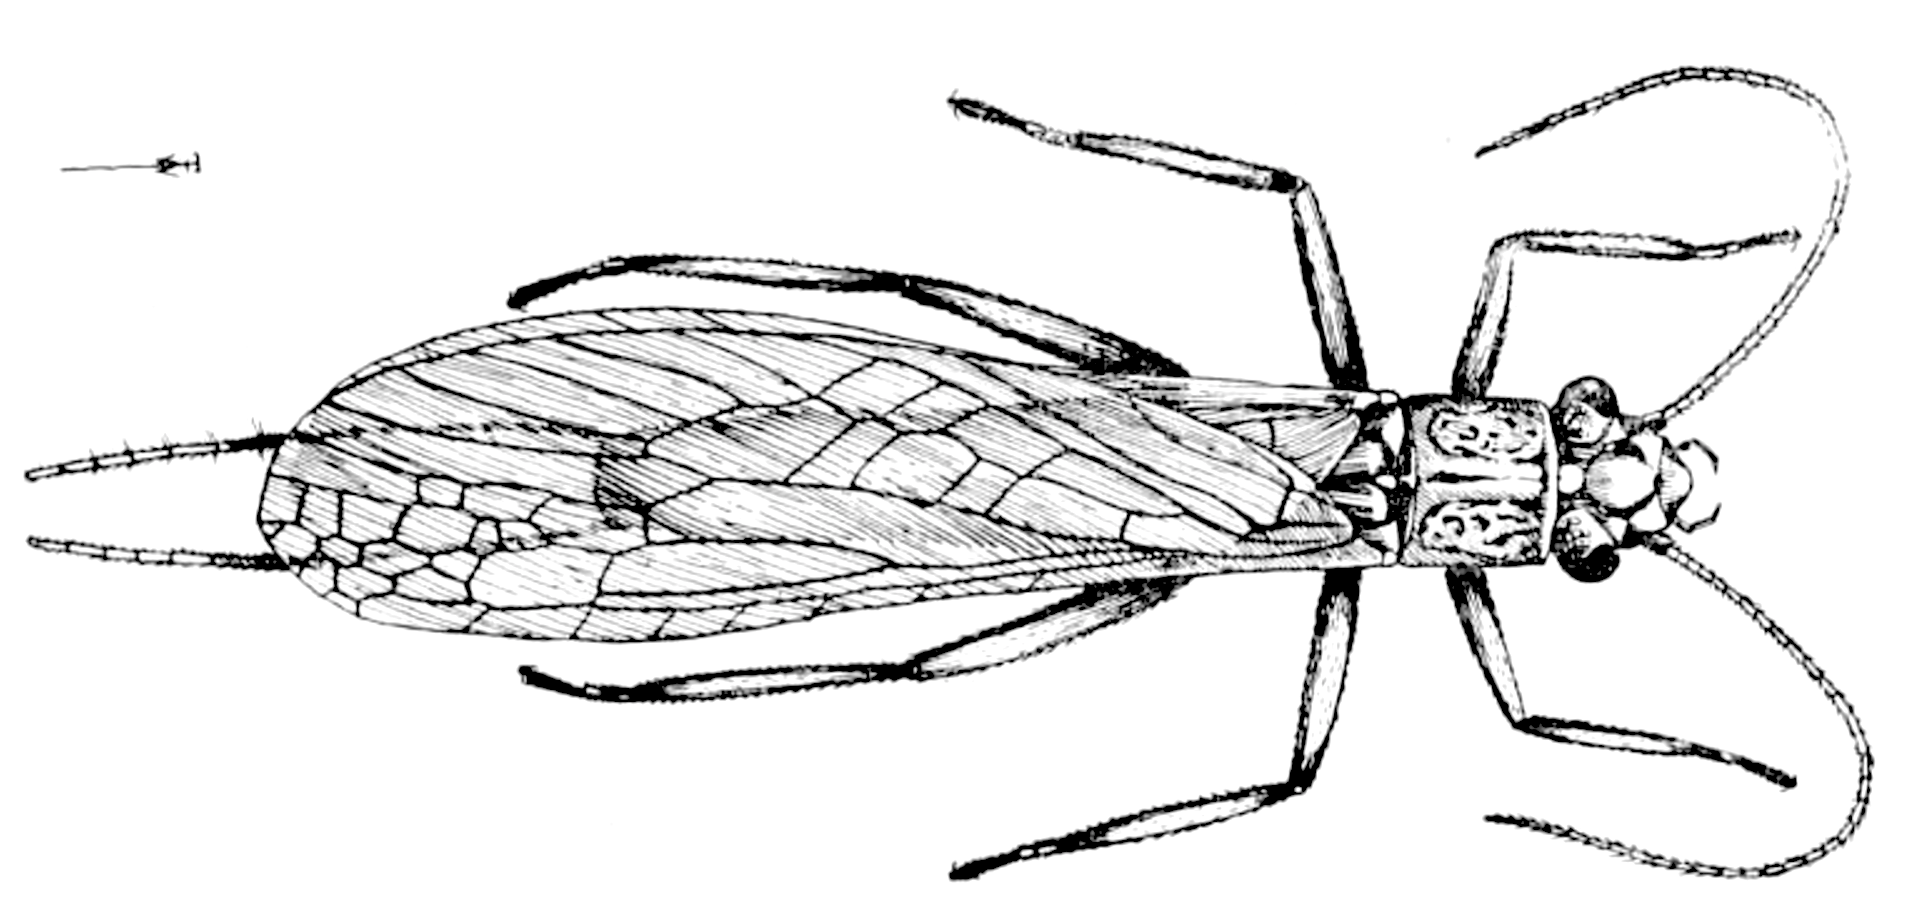
\includegraphics[width=\textwidth]{paleoptera/PerlodidHabitus}
        \caption{}
        \label{fig:perlodid2}
    \end{subfigure}
    \caption{Perlodidae. \textbf{(a)} Wings \citep[modified from][Plate 9, Fig. 1]{bhl29875}; \textbf{(b)} dorsal habitus \citep[modified from][Fig. 12]{bhl29875}}\label{fig:perlodids}
\end{figure}

\subsubsection{Leuctridae (rolled-wing stoneflies)}\index{Leuctridae}
\noindent{}\textit{Diagnostic characters:} Glossae same length as paraglossae; cercus very short composed of one segment; branched gill remnants absent; cubito-anal crossvein arising distal to or from anal cell; 4 or more Cu crossveins on fore wing; 2A forked; fore wings rolled around body.\vspace{3mm}

\noindent{}\textit{Natural history:} Relatively small as adults ($\sim$1 cm long). Naiads feed on plants. More than 350 species are known worldwide, distributed primarily across the Holarctic.\vspace{3mm}

\begin{figure}[ht!]
    \centering
    \begin{subfigure}[ht!]{0.4\textwidth}
        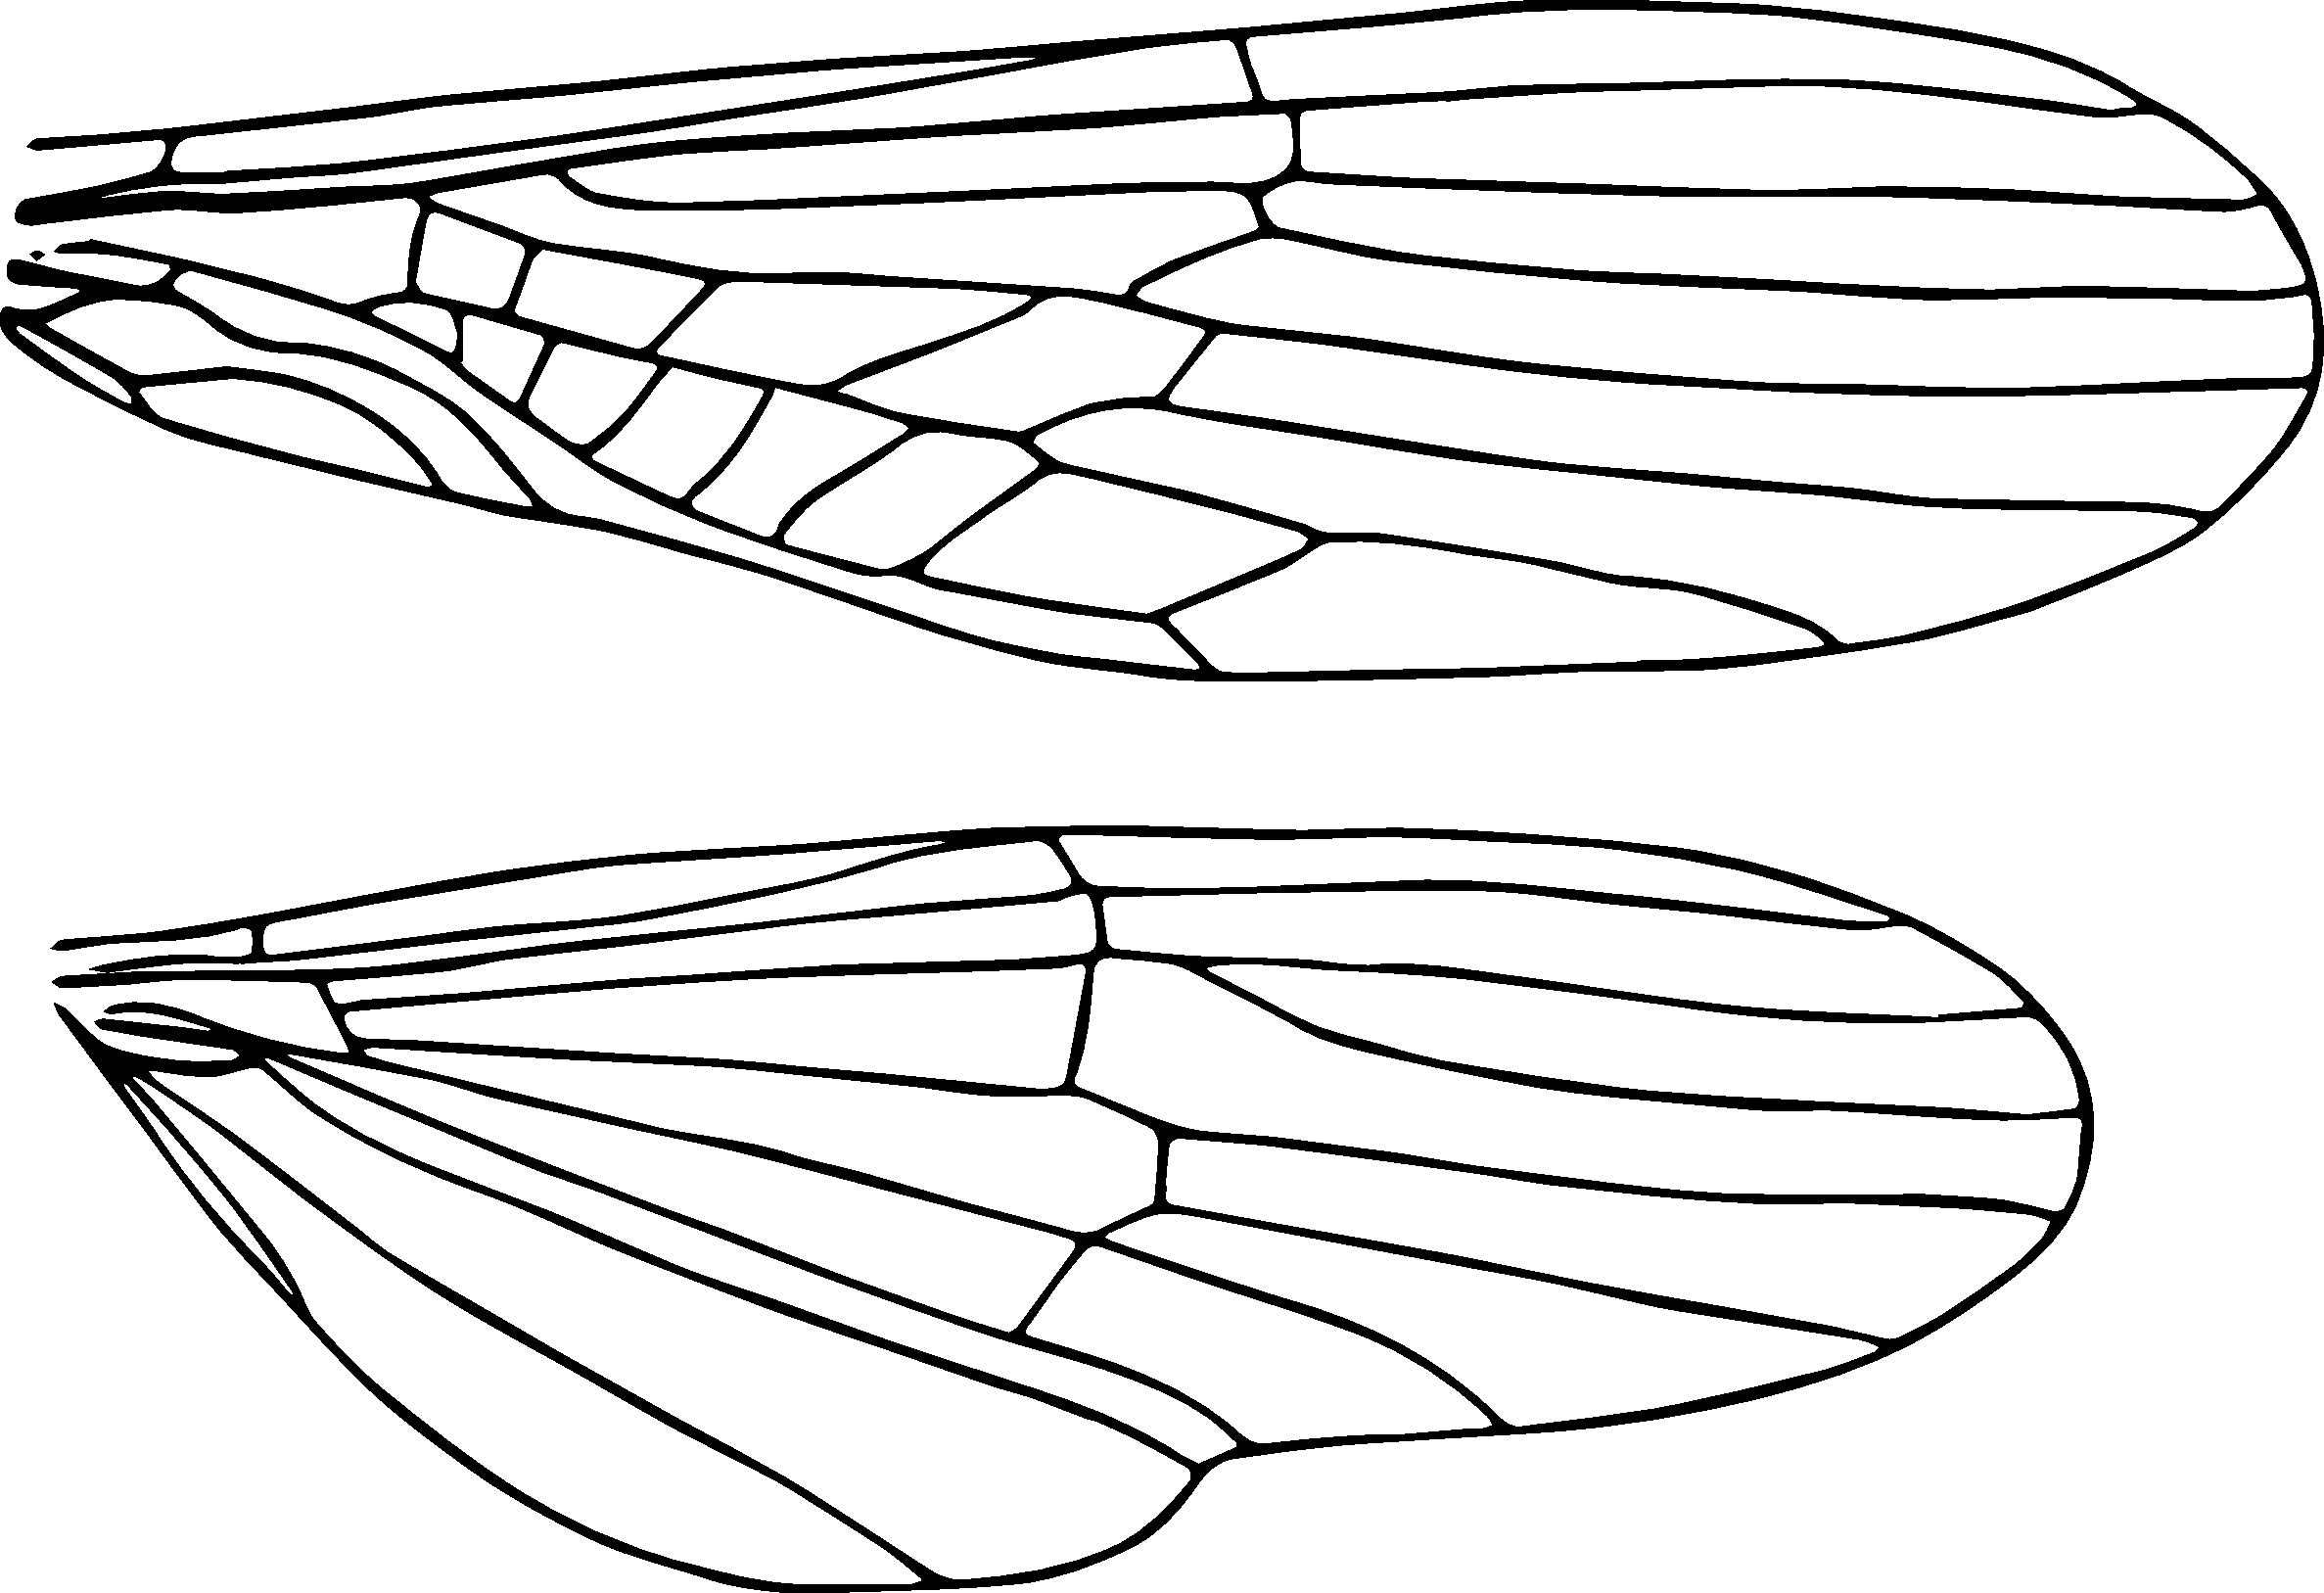
\includegraphics[width=\textwidth]{paleoptera/LeuctridWings}
        \caption{}
        \label{fig:leuctrid1}
    \end{subfigure}
    \qquad
    \begin{subfigure}[ht!]{0.5\textwidth}
        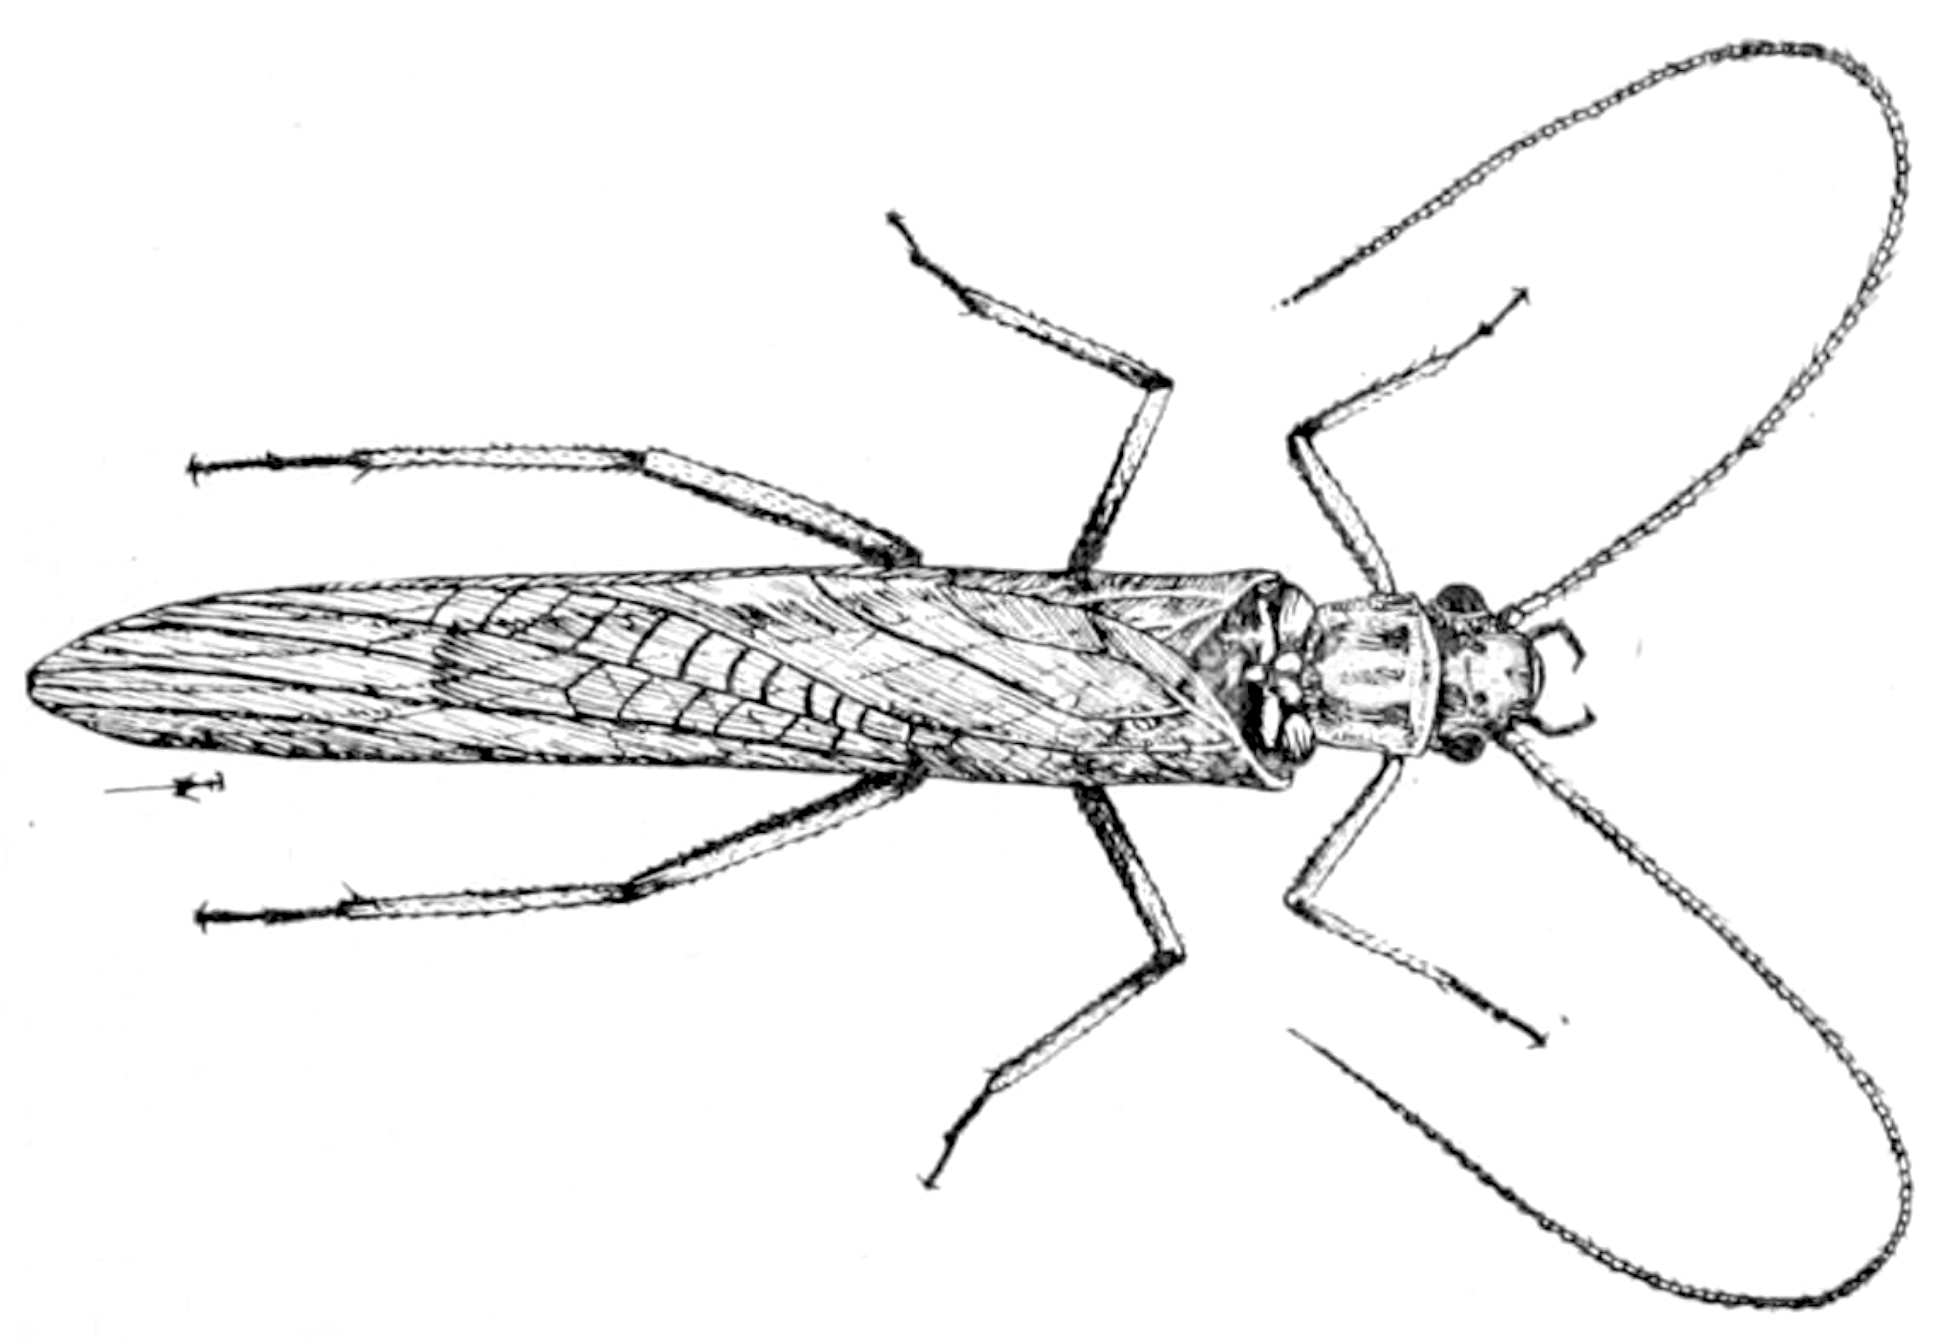
\includegraphics[width=\textwidth]{paleoptera/LeuctridHabitus}
        \caption{}
        \label{fig:leuctrid2}
    \end{subfigure}
    \caption{Leuctridae. \textbf{(a)} Wings \citep[redrawn from][Plate 32, Fig. 1]{bhl29875}; \textbf{(b)} dorsal habitus \citep[modified from][Fig. 26]{bhl29875}}\label{fig:leuctrids}
\end{figure}

\subsubsection{Capniidae (winter stoneflies)}\index{Capniidae}
\noindent{}\textit{Diagnostic characters:} Glossae same length as paraglossae; cercus with at least 4 segments; gill remnants absent; cubito-anal crossvein arising distal to or from anal cell; 1--2 or more Cu crossveins on fore wing; 2A not forked.\vspace{3mm}

\noindent{}\textit{Natural history:} Similar in size, habitus, and diversity to Leuctridae. Adults are active in winter. Naiads are lotic, primarily in the hyporheic zone (beneath the stream bed), and rarely collected.\vspace{3mm}

\begin{figure}[ht!]
    \centering
    \begin{subfigure}[ht!]{0.4\textwidth}
        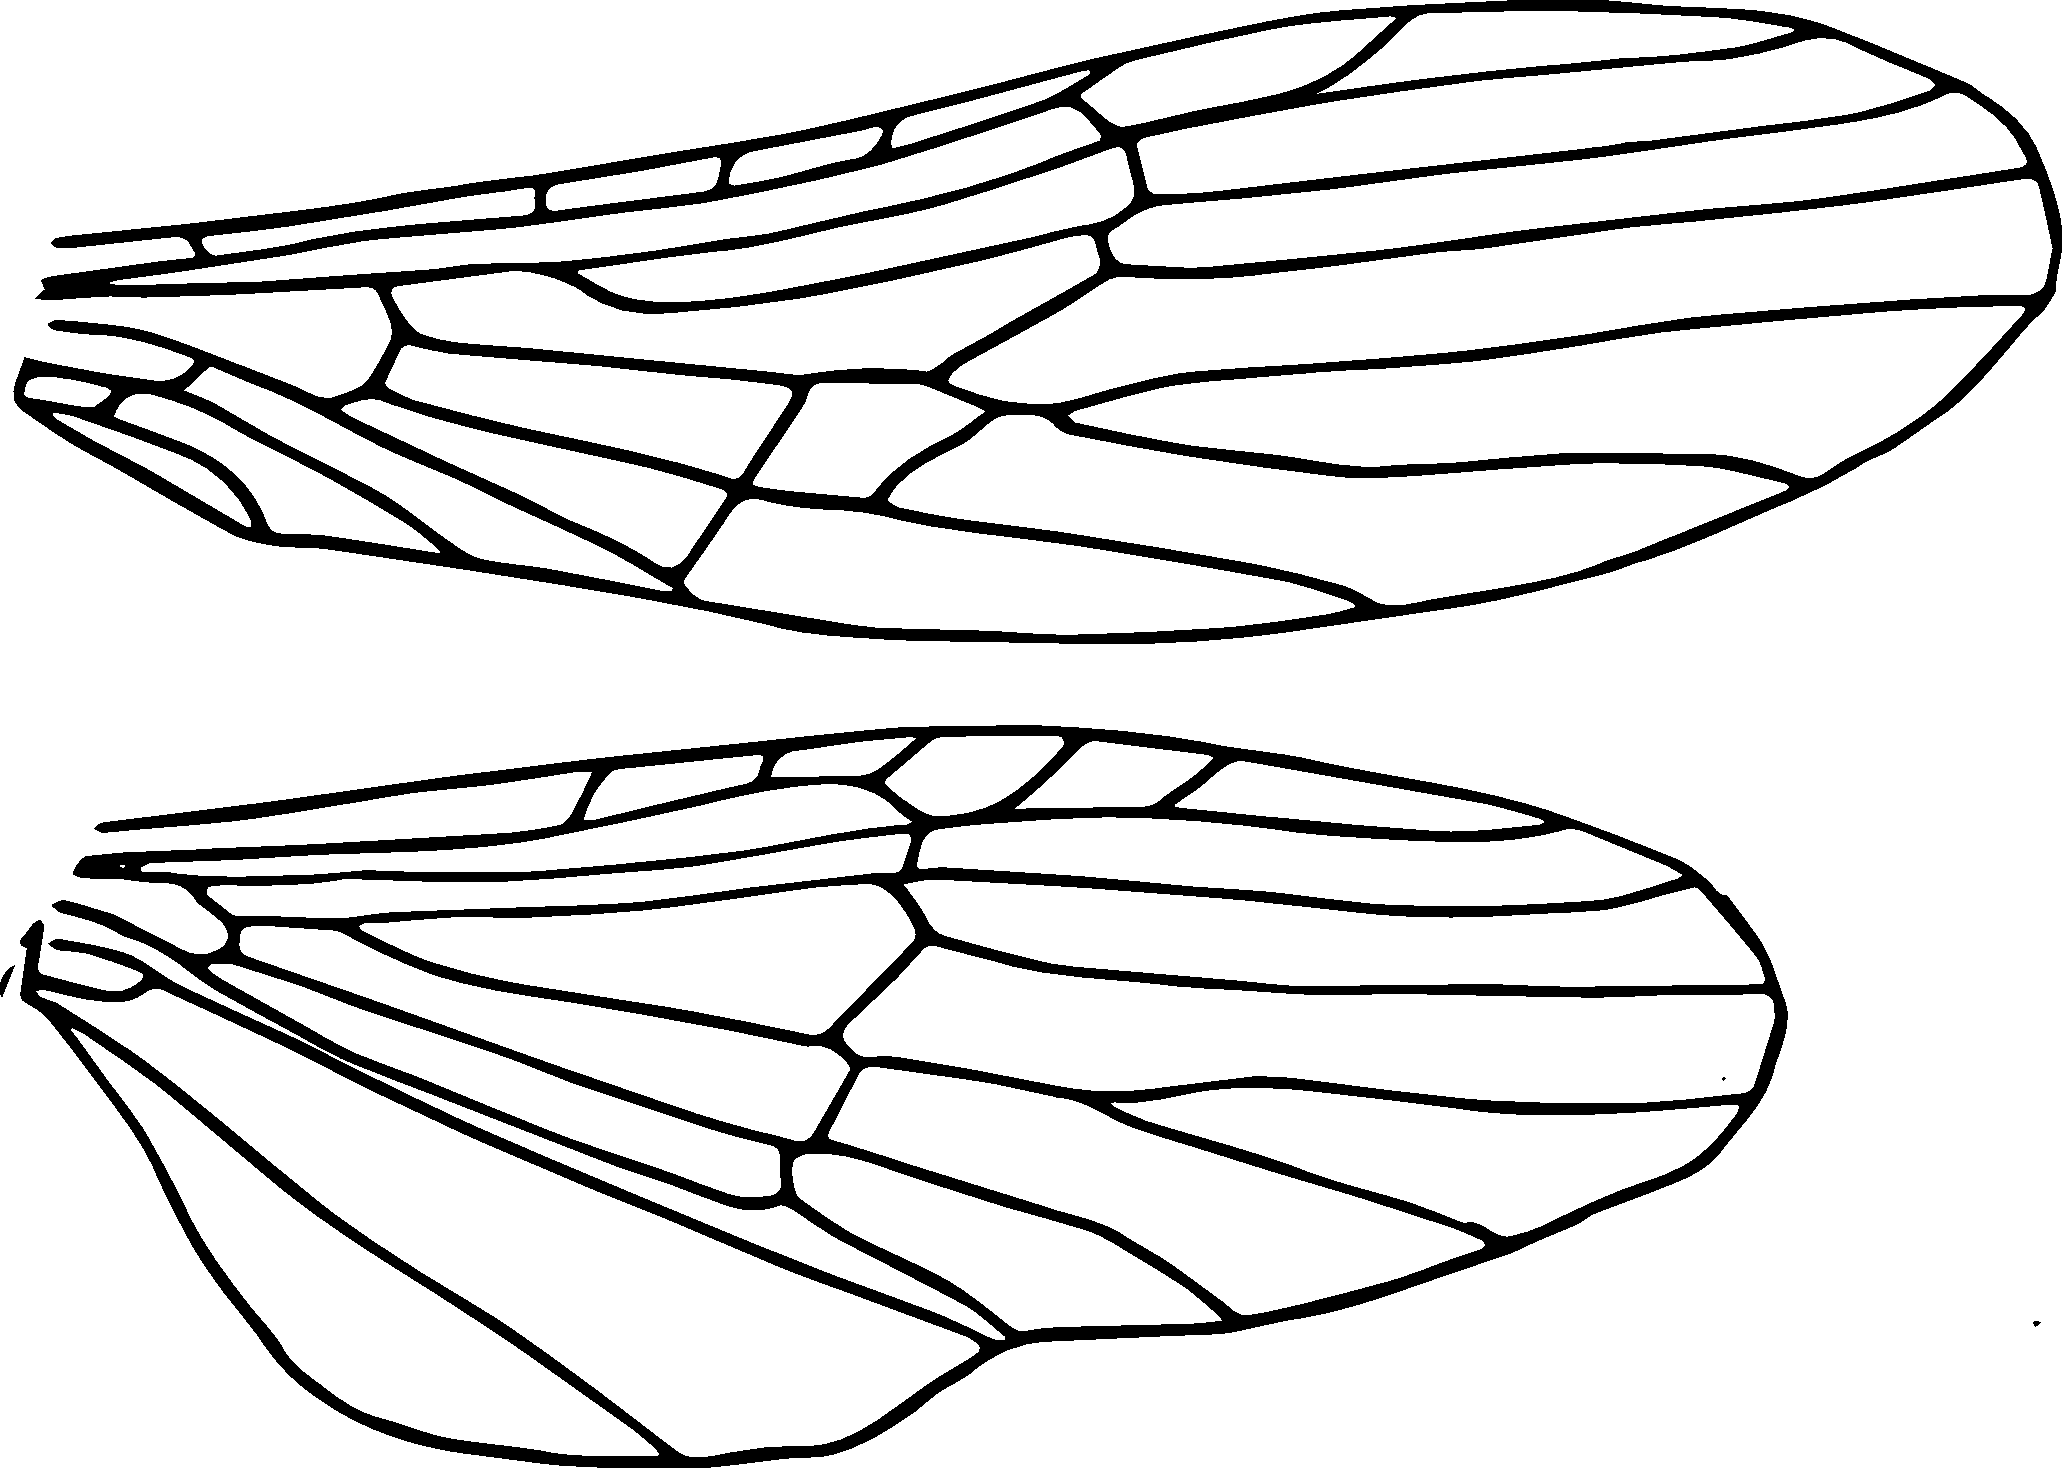
\includegraphics[width=\textwidth]{paleoptera/CapniidWings}
        \caption{}
        \label{fig:capniid1}
    \end{subfigure}
    \qquad
    \begin{subfigure}[ht!]{0.52\textwidth}
        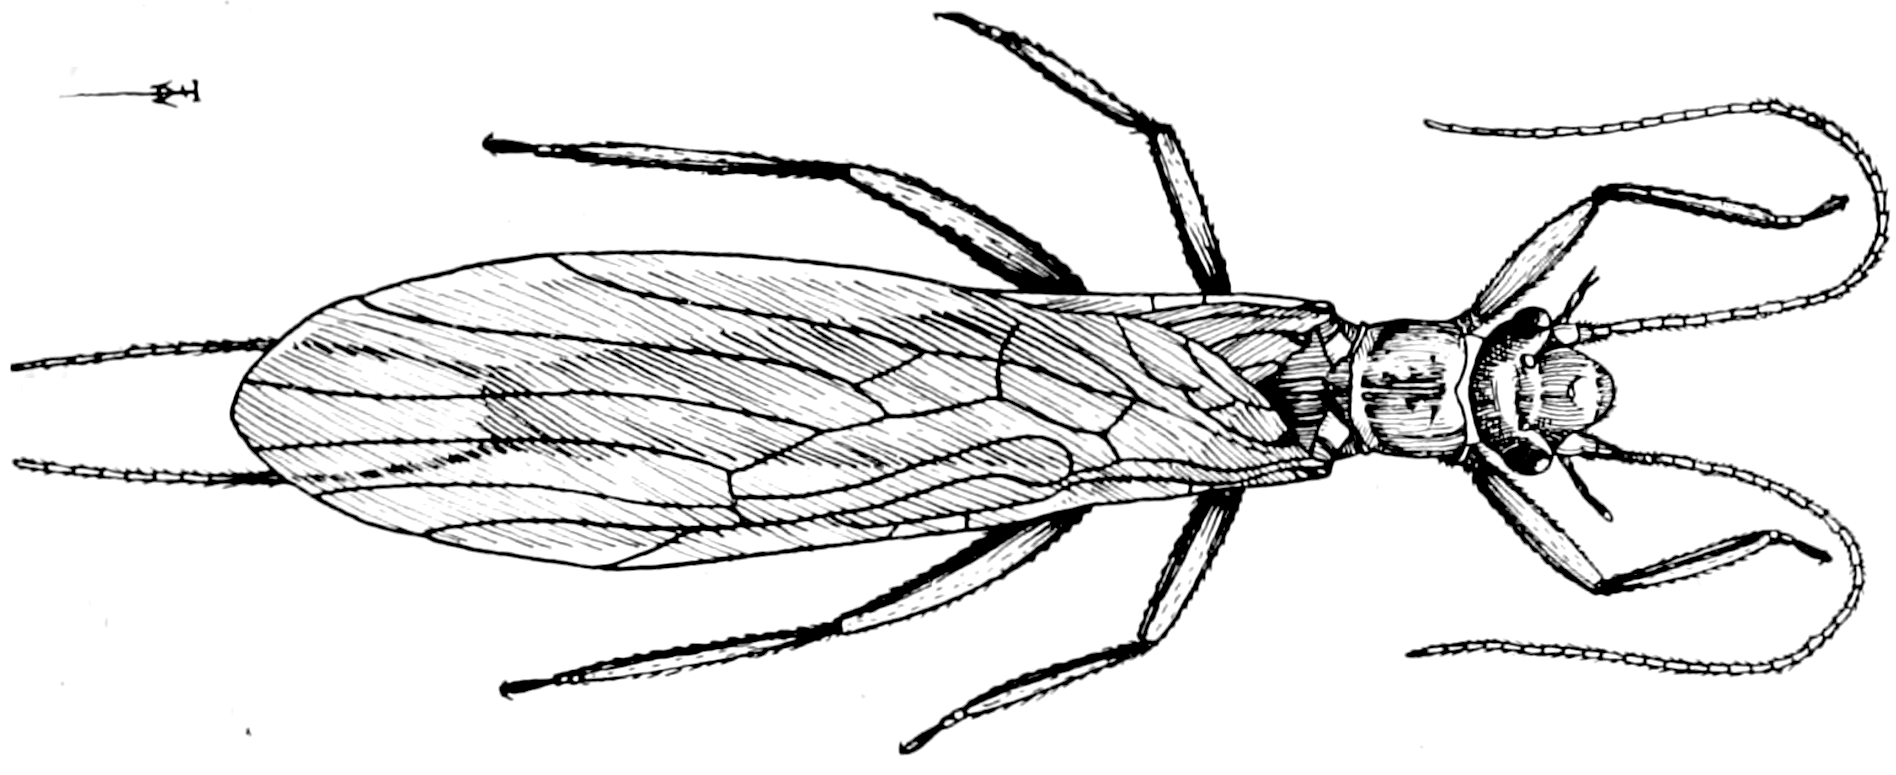
\includegraphics[width=\textwidth]{paleoptera/CapniidHabitus}
        \caption{}
        \label{fig:capniid2}
    \end{subfigure}
    \caption{Capniidae. \textbf{(a)} Wings \citep[modified from][Plate 47, Fig. 2]{bhl29875}; \textbf{(b)} habitus \citep[redrawn from][Fig. 28]{bhl29875}}\label{fig:capniids}
\end{figure}

\begin{theo}
{}How did wings evolve? Did they develop \textit{de novo} or from existing structures? Why? Based on what you have learned in this course, what is the most plausible explanation for the origin of wings?
\end{theo}

\section*{Test yourself}
If you were given a naiad (of the families we looked at in lab) could you identify it by sight? What about the adult form?\vspace{3mm}

\noindent{}After listening to the class discussion, which hypothesis do you think most accurately explains the origin of wings in insects and why?\vspace{3mm}

\noindent{}We talked about several adaptations one can see in paleopterans---for feeding, flying, mating, living in aquatic habitats, \textit{etc}. Which three are the most significant to you and why?

\clearpage
\thispagestyle{empty}
